\chapter{Fundamentos de Herramientas Numéricas}






\newpage

\section{Xcompac3D}

The finite difference code Incompact3d [33, 34] is employed to solve equations 1–3. For the spatial differentiation, sixth‑order centered compact schemes are used [35]. The time integration is performed using a second‑order Adams–Bashforth scheme with an approximated time step of 10⁻³ due to the CFL restriction. The N‑S equations are solved using the fractional‑step method, where the Poisson equation is solved in the spectral space. The code is parallelized under the MPI paradigm and uses the 2DCOMP&FFT library [36]. For more information about the code Incompact3d visit http://www.incompact3d.com/.

BUSCAR LAS REFERENCIAS. TRADUCIR, AGREGAR, MODIFICAR ETC ETC

\subsection{Validación}

\section{Orr-Somerfeld Mixed Convection}

\subsection{Validación}




\begin{comment}


\section{Validaciones de Simulaciones de Canales Periódicos con Convección Forzada}

\subsection{Distintos valores de Prandt}

\begin{figure}[H]
 \centering
  \subfloat[]{
    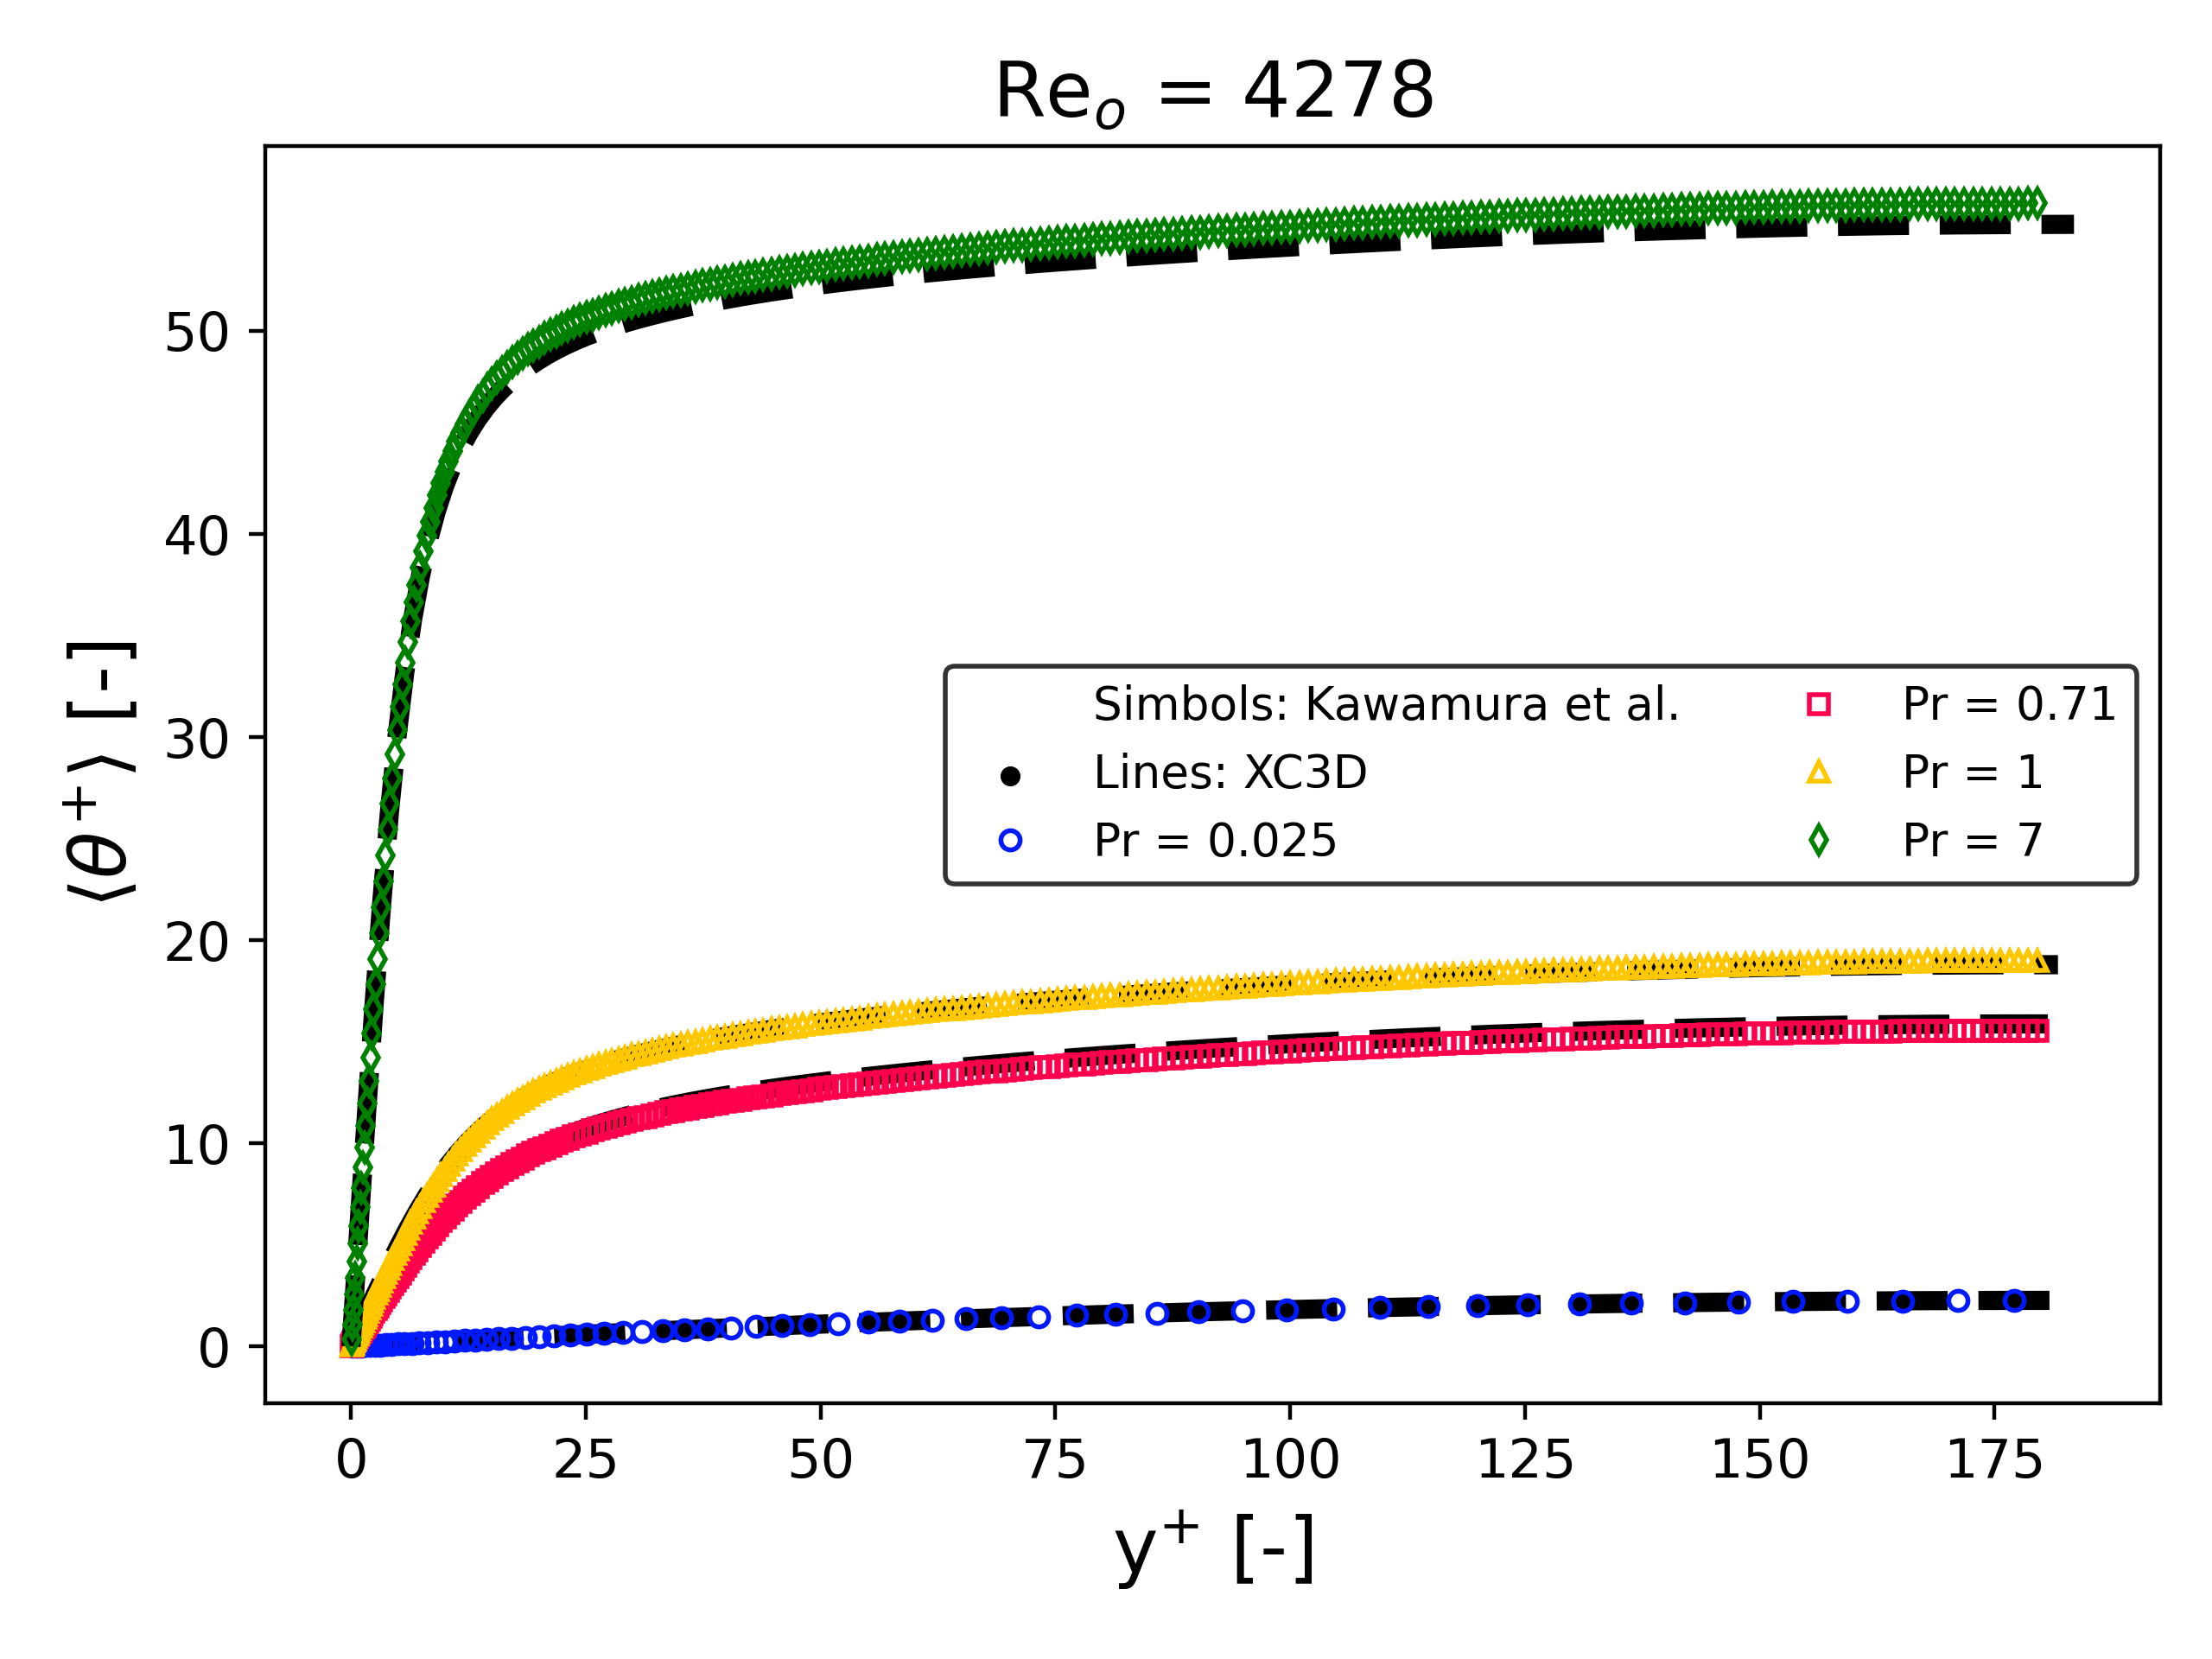
\includegraphics[width=0.49\textwidth]{results/kawamura/prandts/tep_theta.png}
    \label{fig:phi_mean_kawa}}  
    \subfloat[]{
    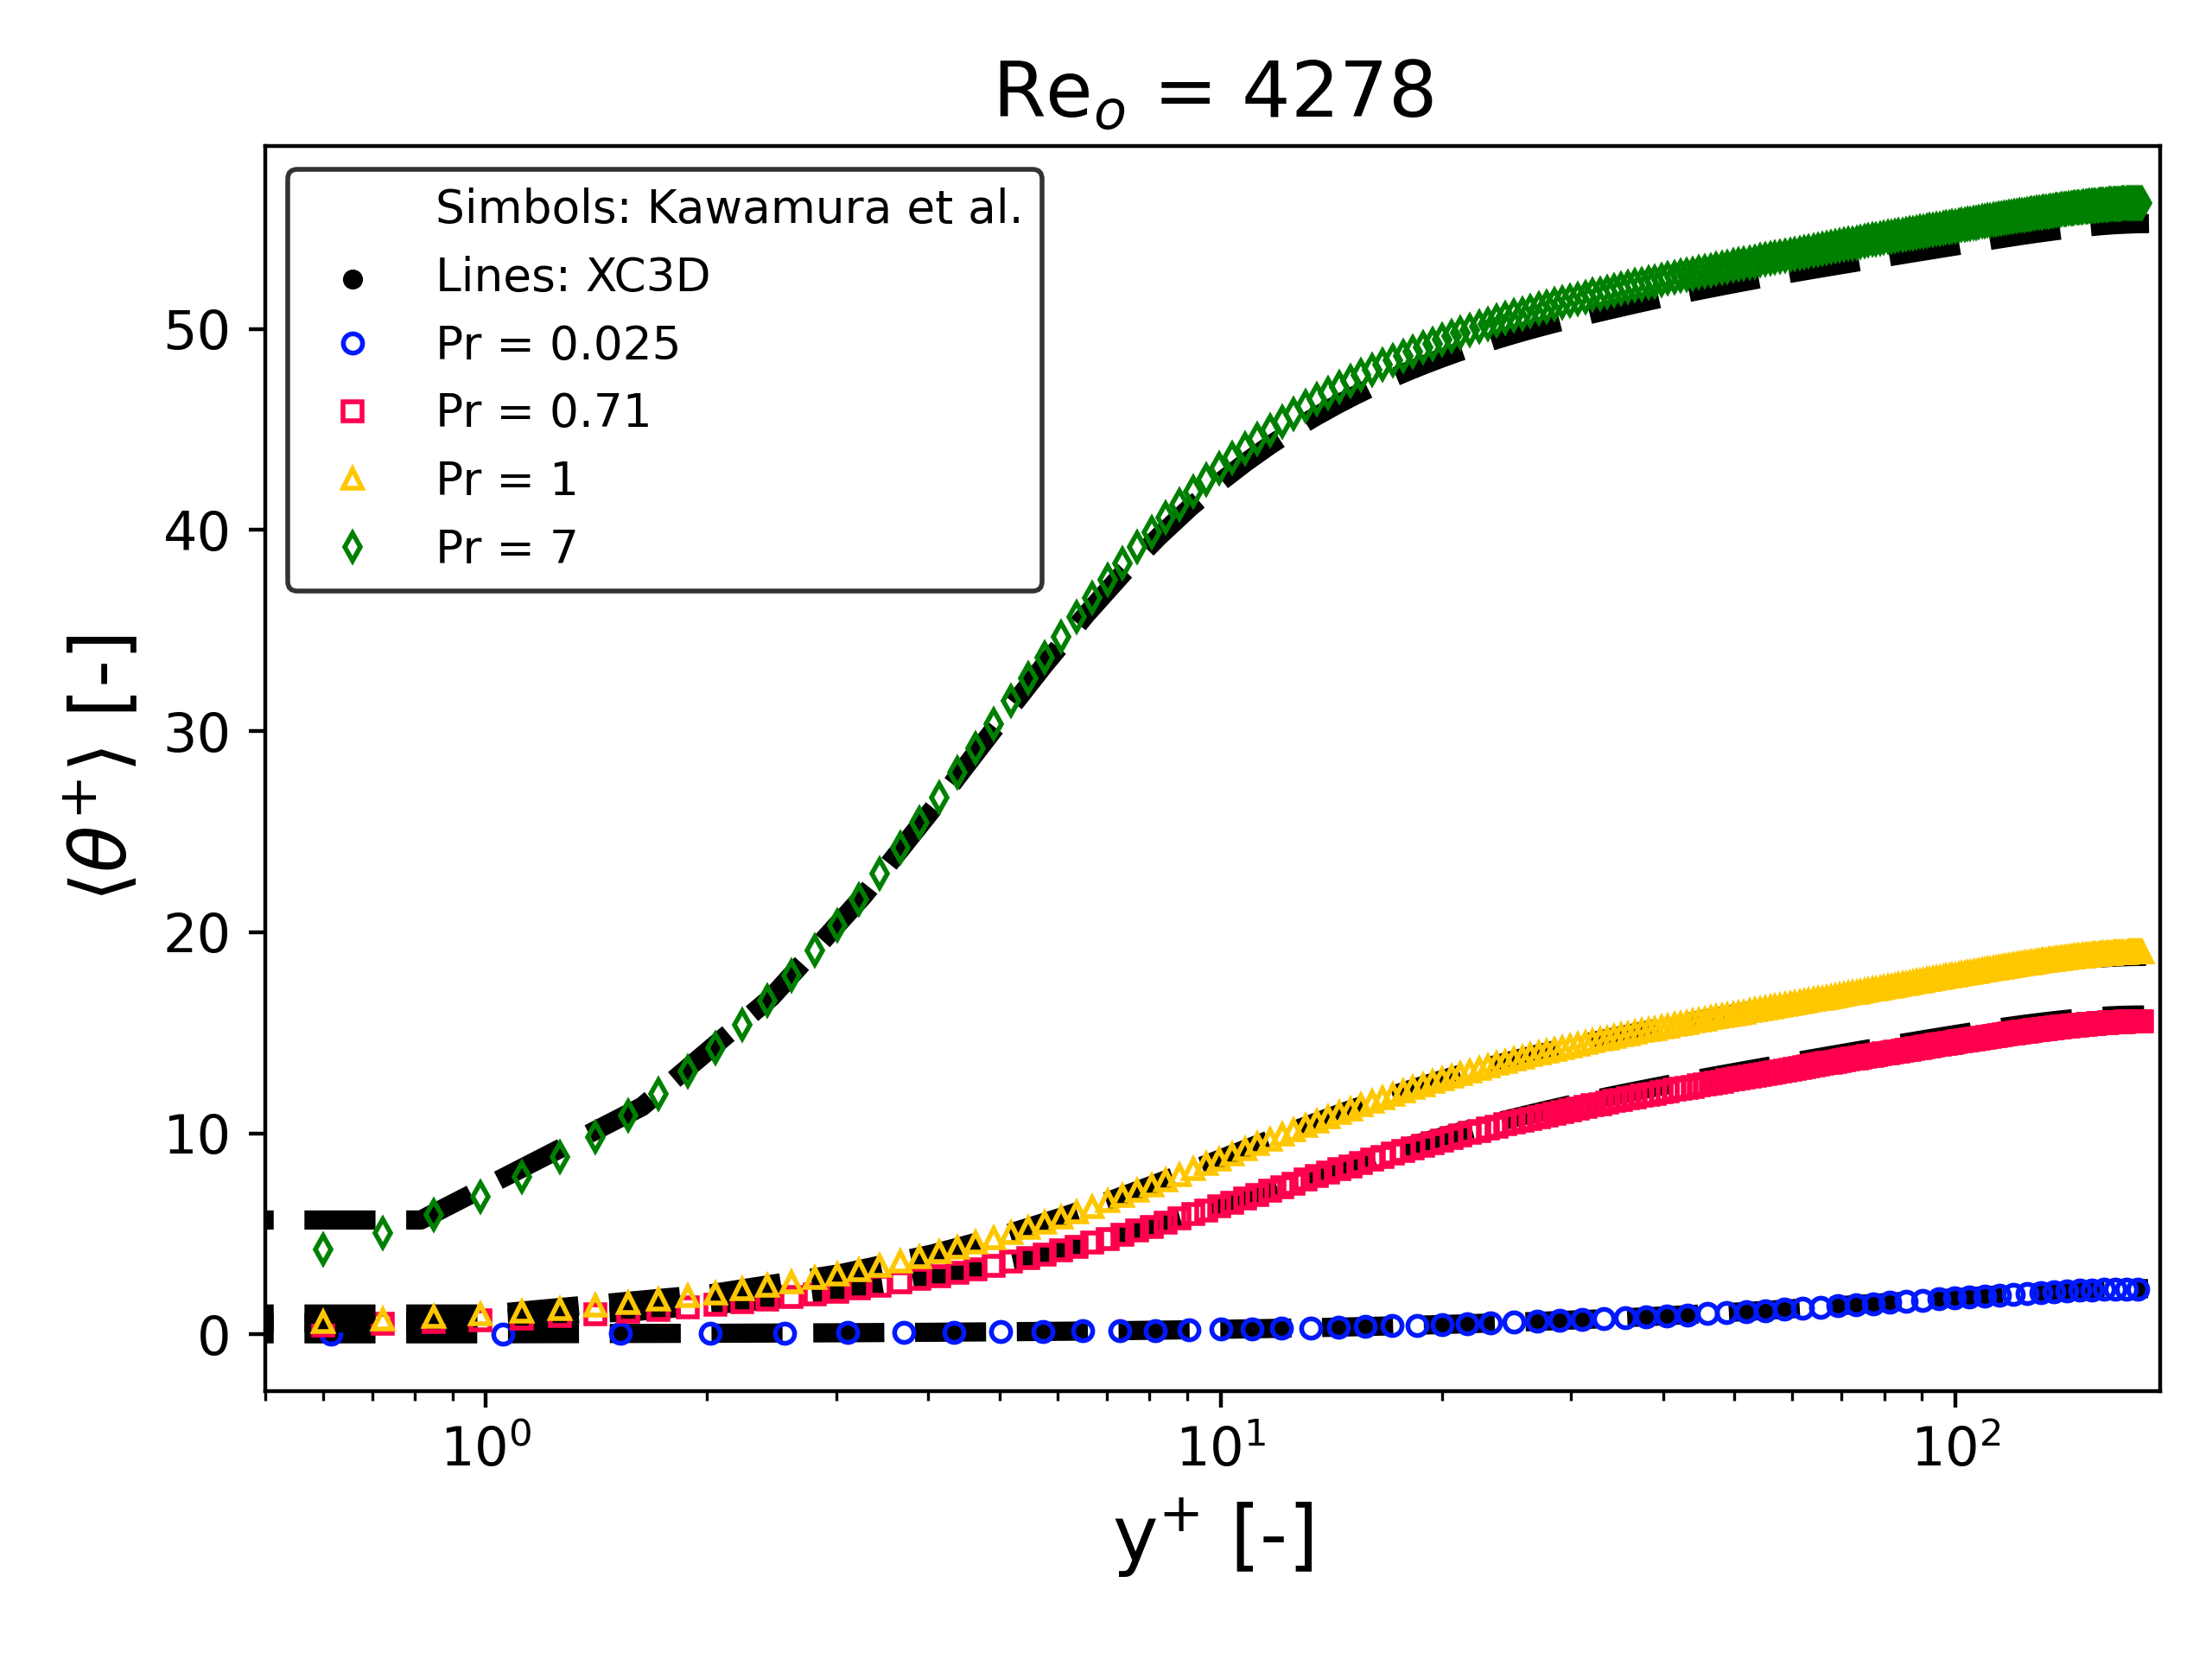
\includegraphics[width=0.49\textwidth]{results/kawamura/prandts/tep_theta_log.png}
    \label{fig:phi_mean_log_kawa}}  
 \caption{Perfiles de temperatura media $\langle  \theta^+ \rangle$ en unidades de pared. a) Escala lineal. b) Escala logaritmica en en y.} 
 \label{fig:kawamura_1}
\end{figure}

\begin{figure}[H]
 \centering
  \subfloat[]{
    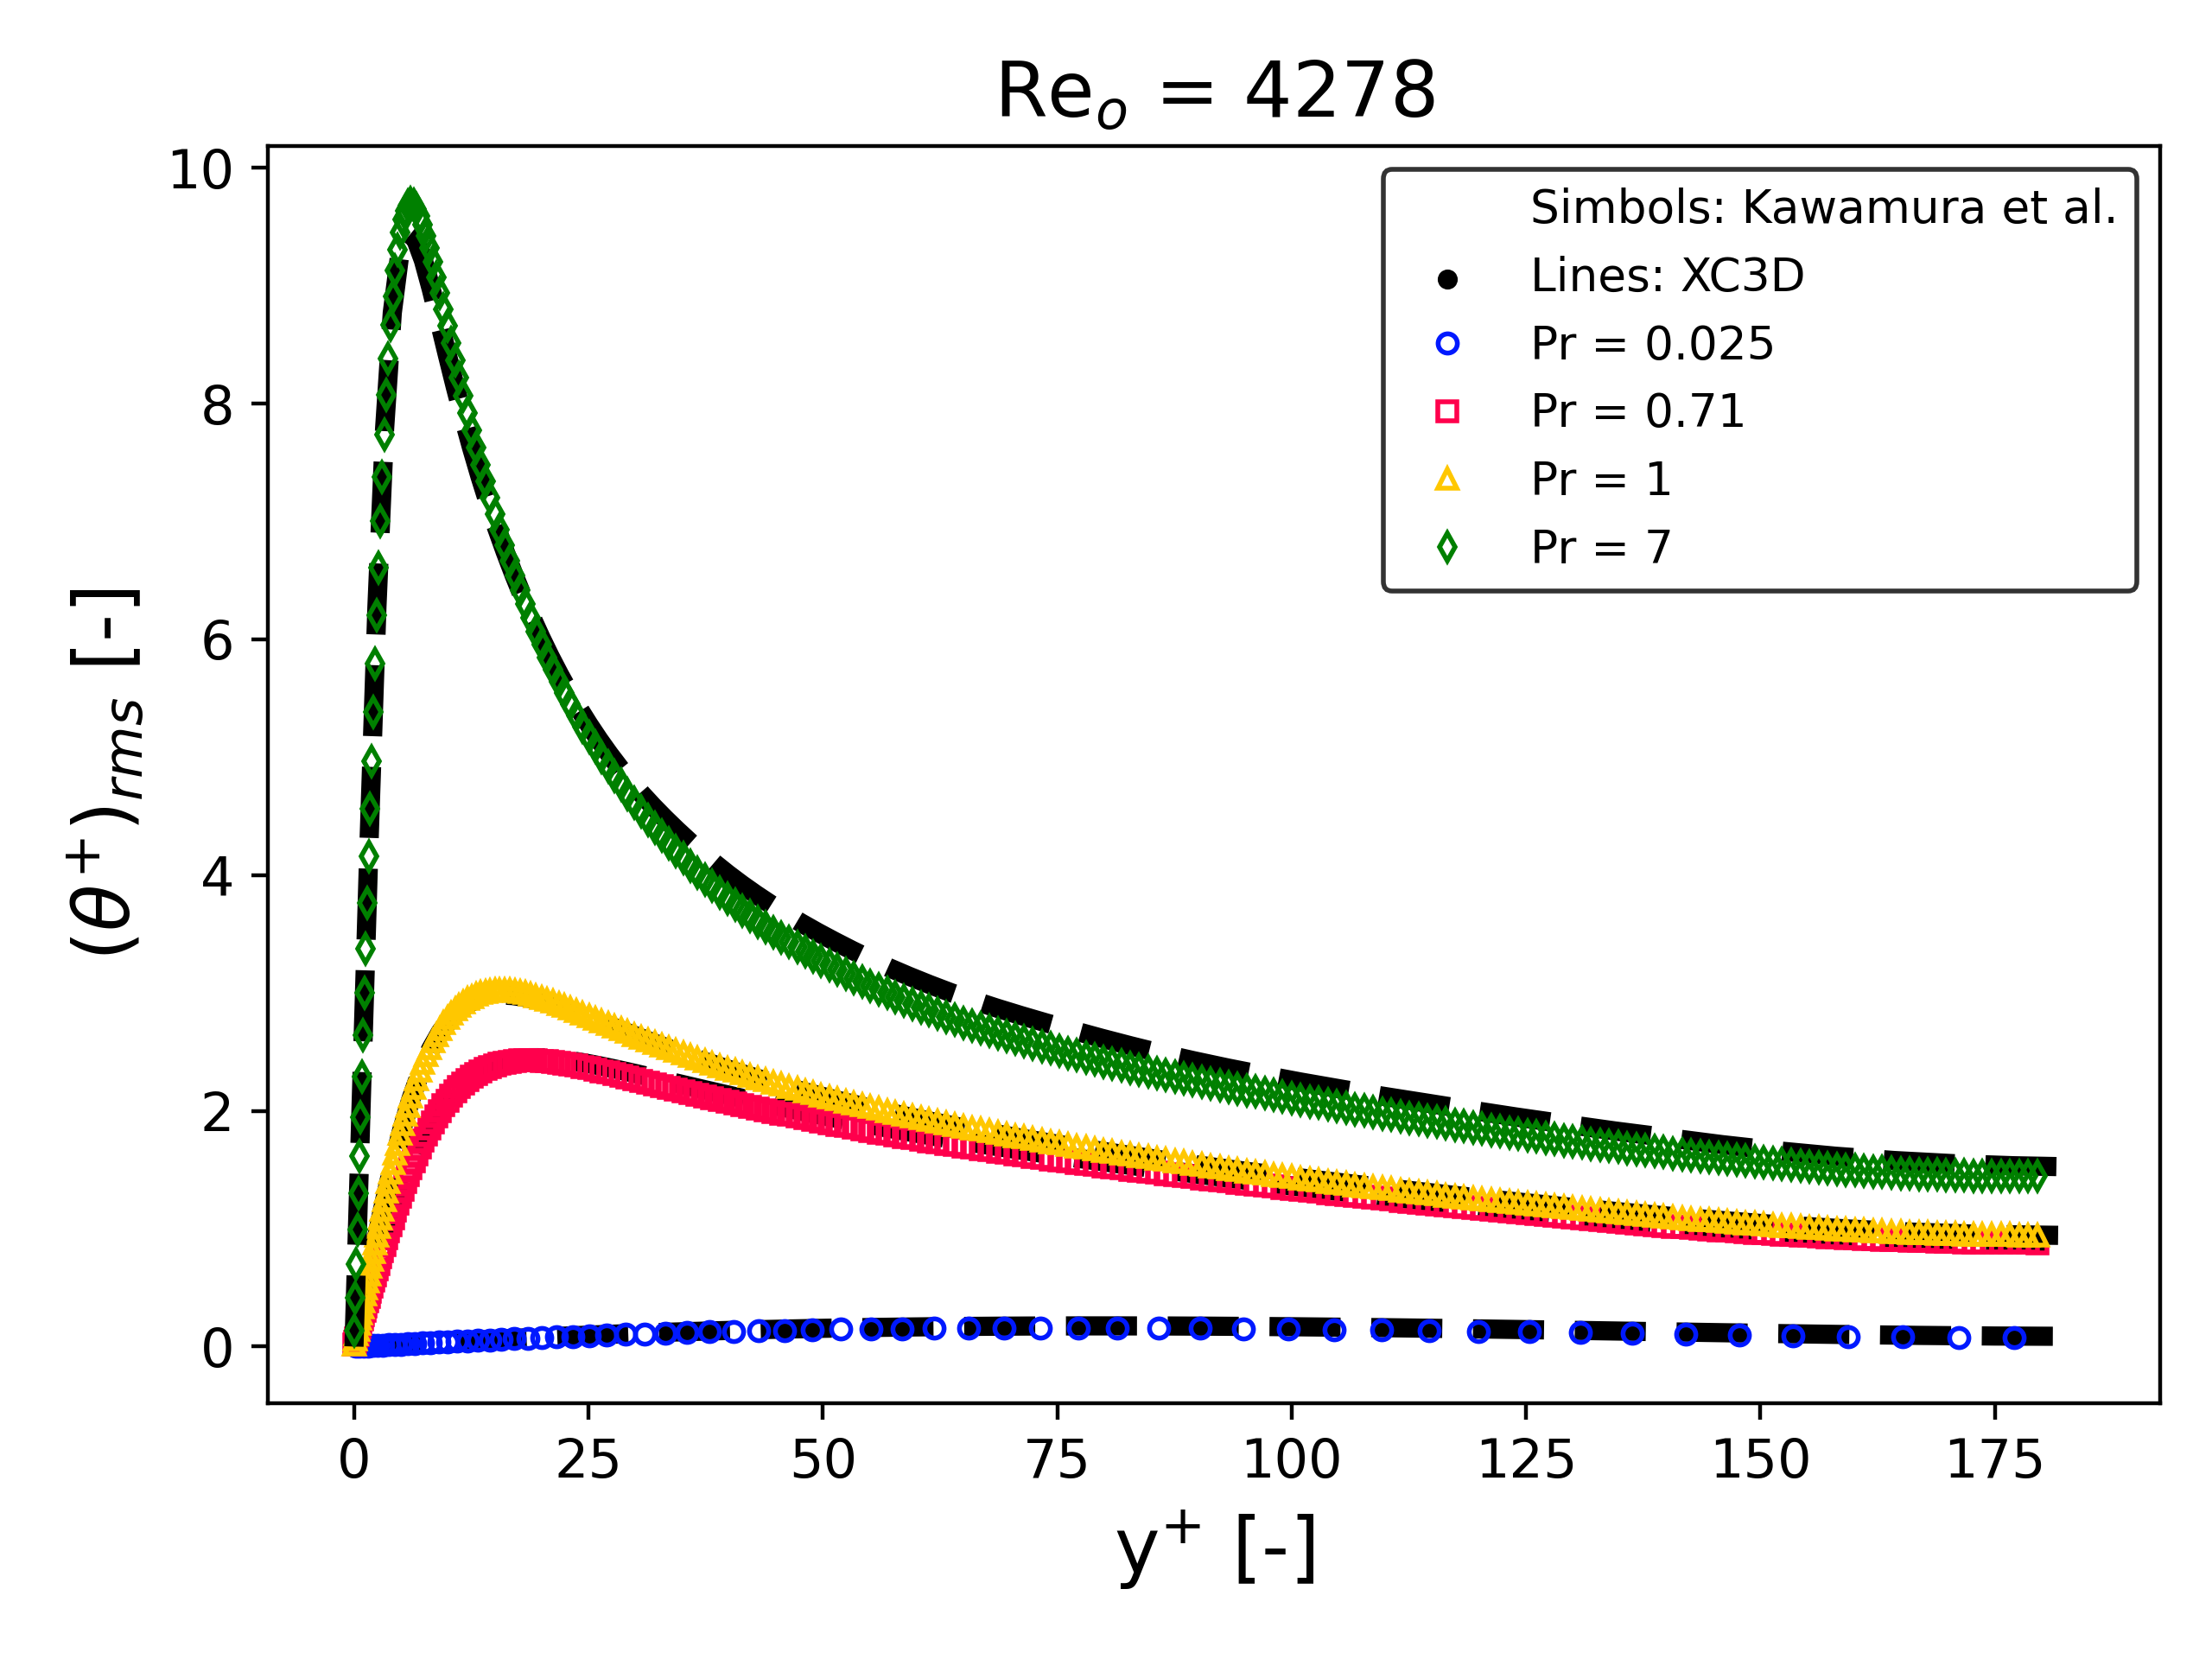
\includegraphics[width=0.33\textwidth]{results/kawamura/prandts/tep_thetap_rms.png}
    \label{fig:phi_rms_kawa}}  
  \subfloat[]{
    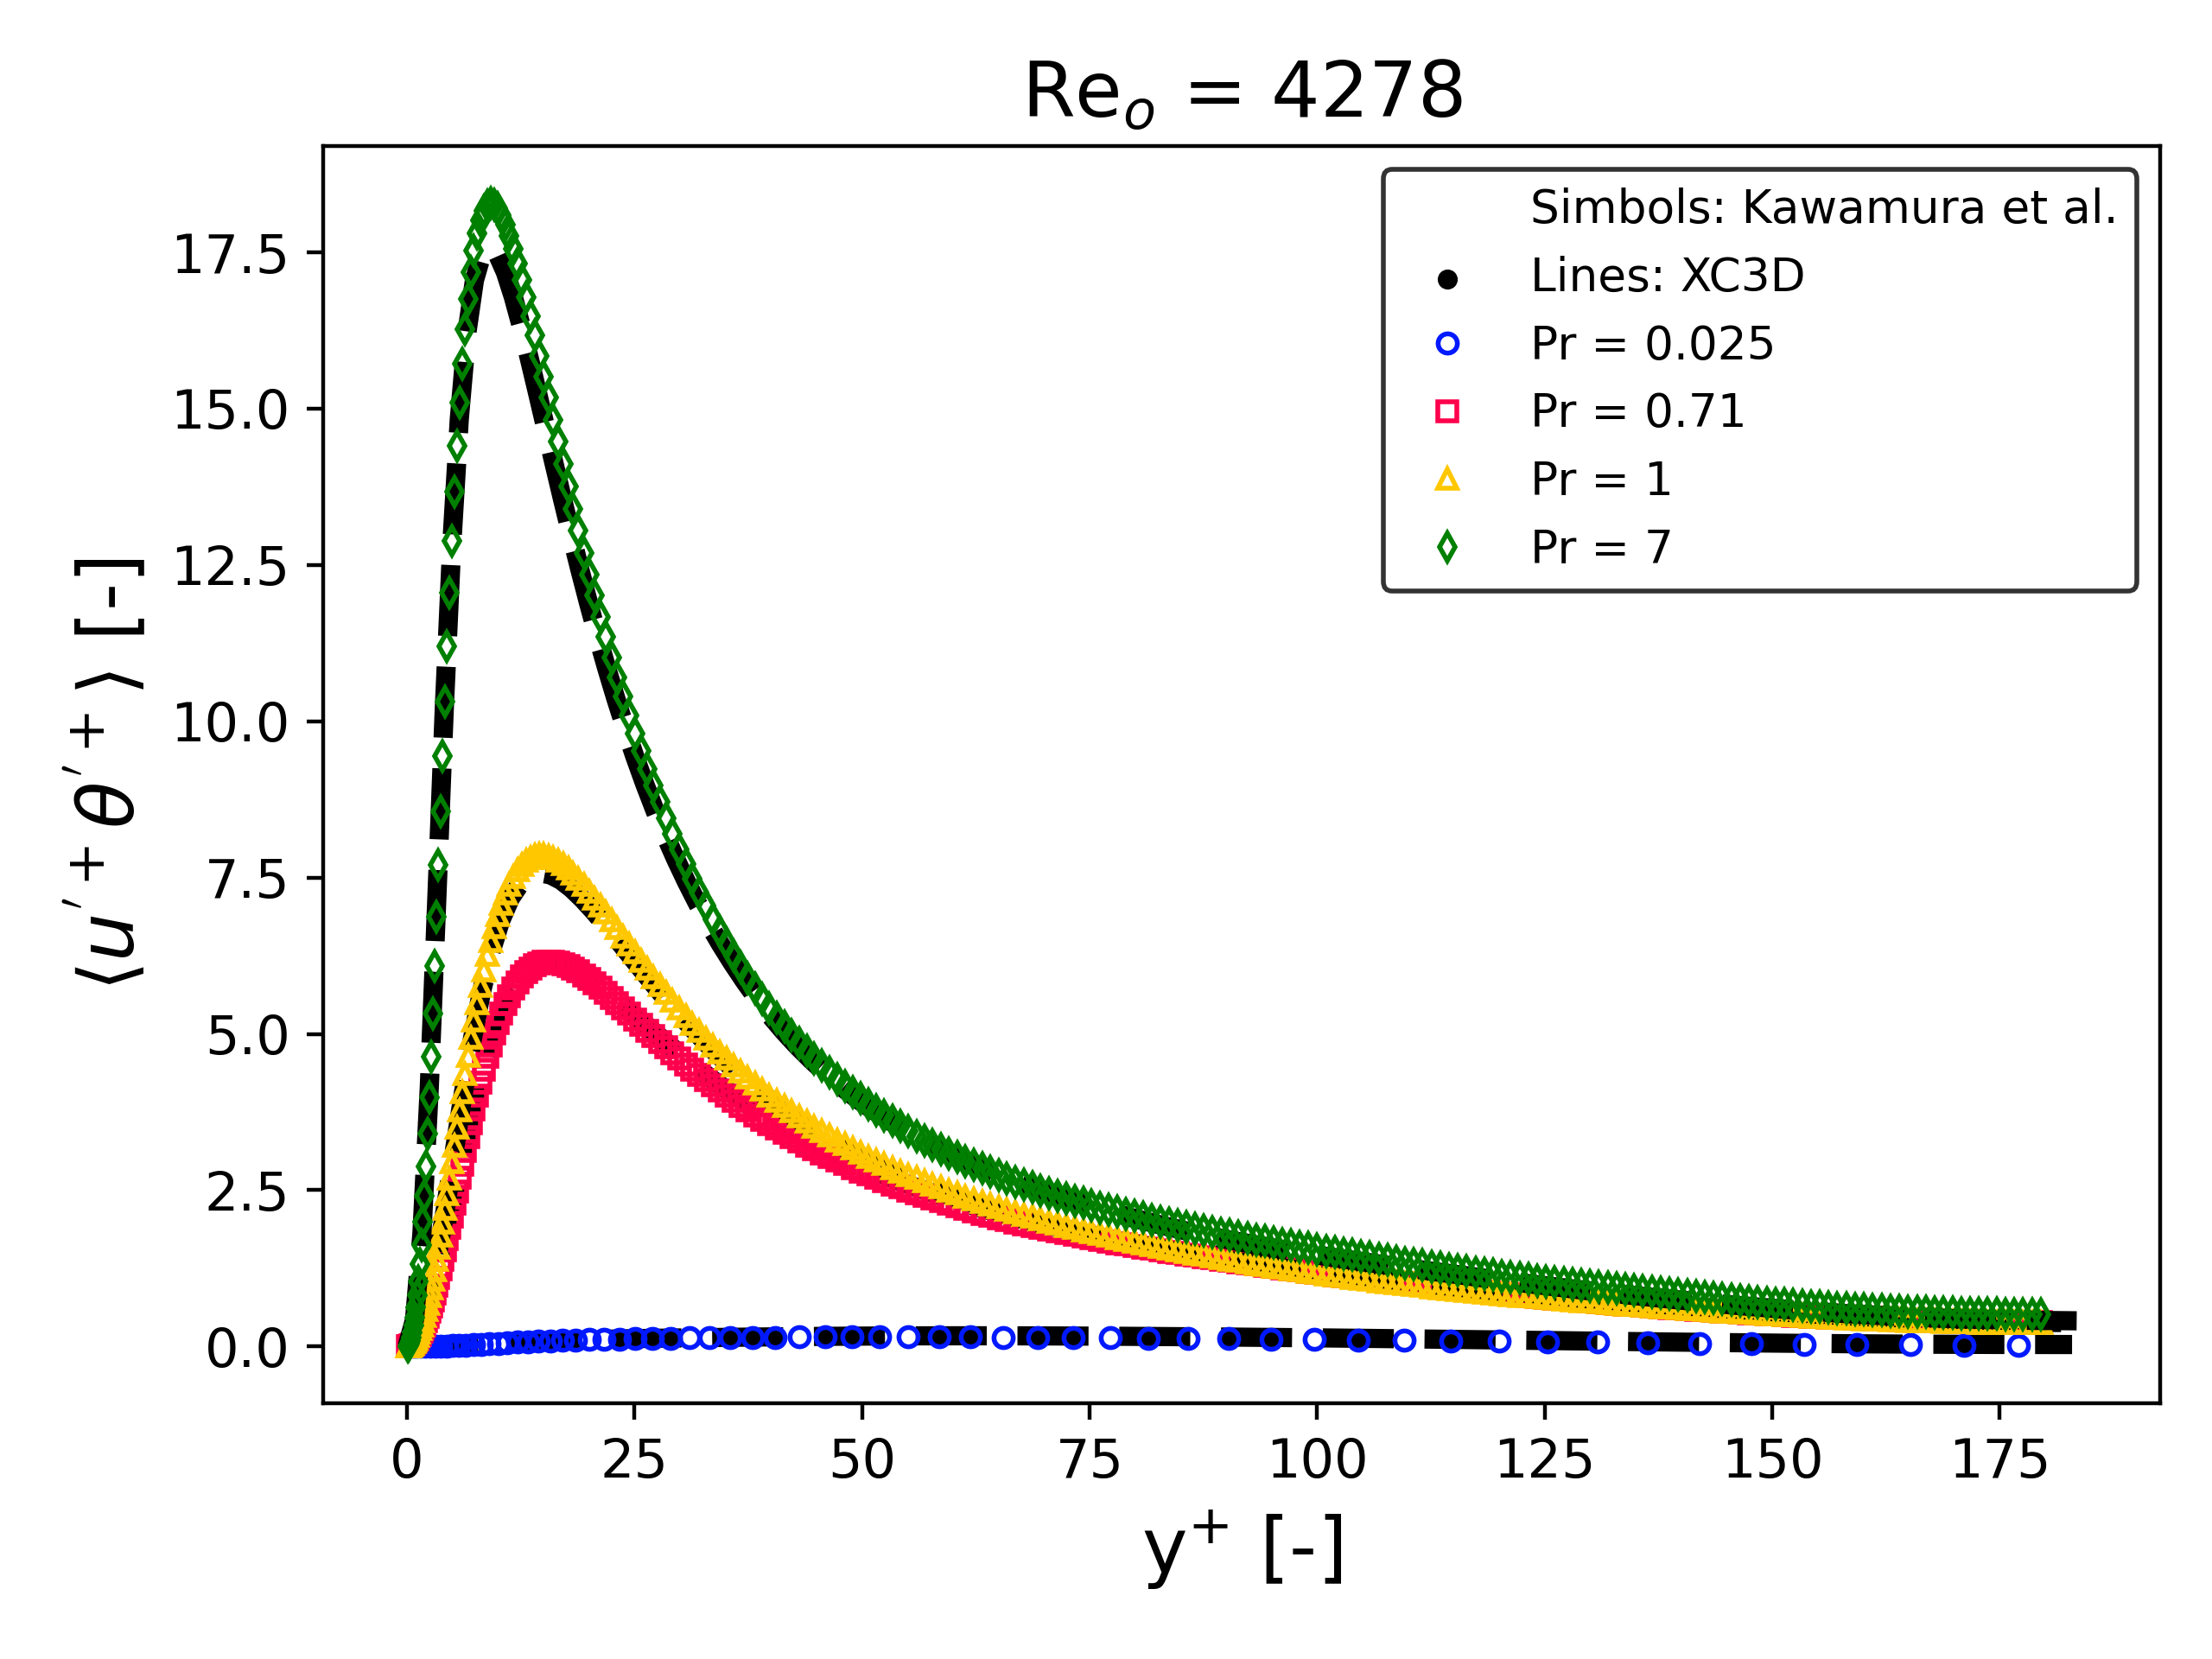
\includegraphics[width=0.33\textwidth]{results/kawamura/prandts/tep_up_thetap.png}
    \label{fig:phi_up_thetap_kawa}}
  \subfloat[]{
    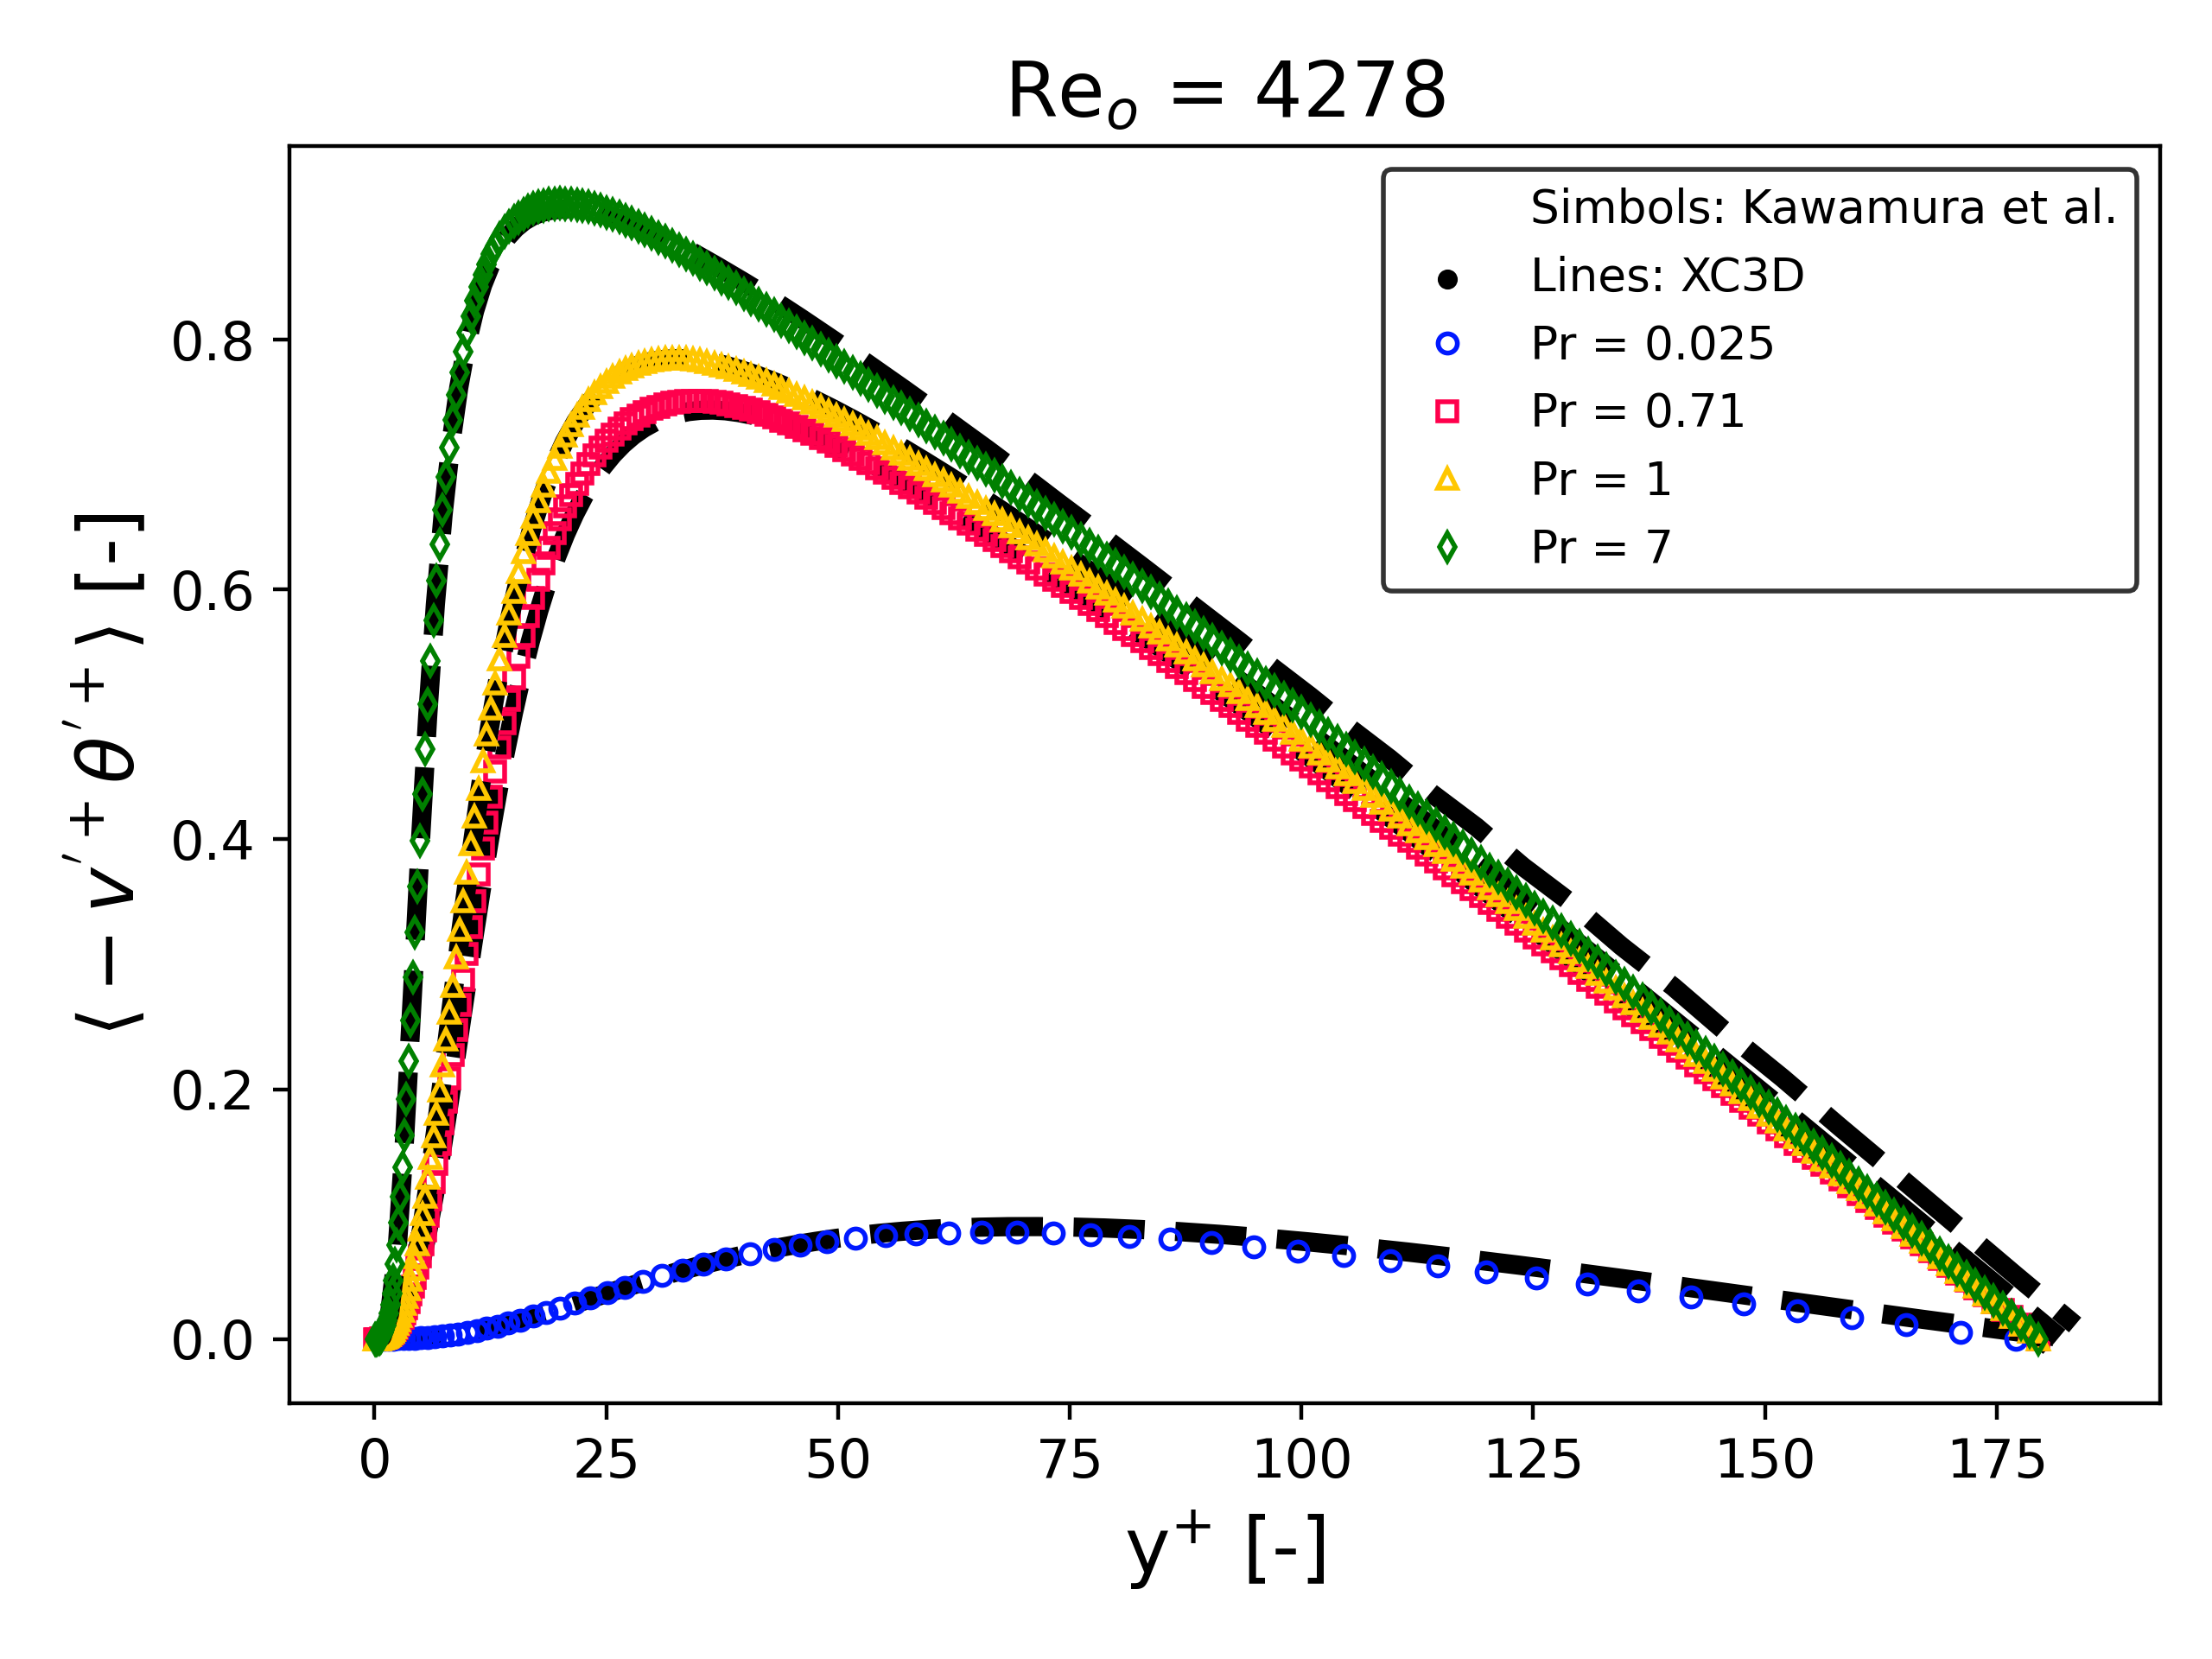
\includegraphics[width=0.33\textwidth]{results/kawamura/prandts/tep_vp_thetap.png}
    \label{fig:phi_vp_thetap_kawa}}  
    
   \caption{a) Fluctuaciones de la temperatura.  b) Flujo turbulento de calor en la dirección X. c) Flujo turbulento de calor en la dirección Y.} 
 \label{fig:kawamura_2}
\end{figure}

\subsection{Comparación de mallas para el caso $\mathbf{Pr=0.71}$}

\begin{figure}[H]
 \centering
  \subfloat[]{
    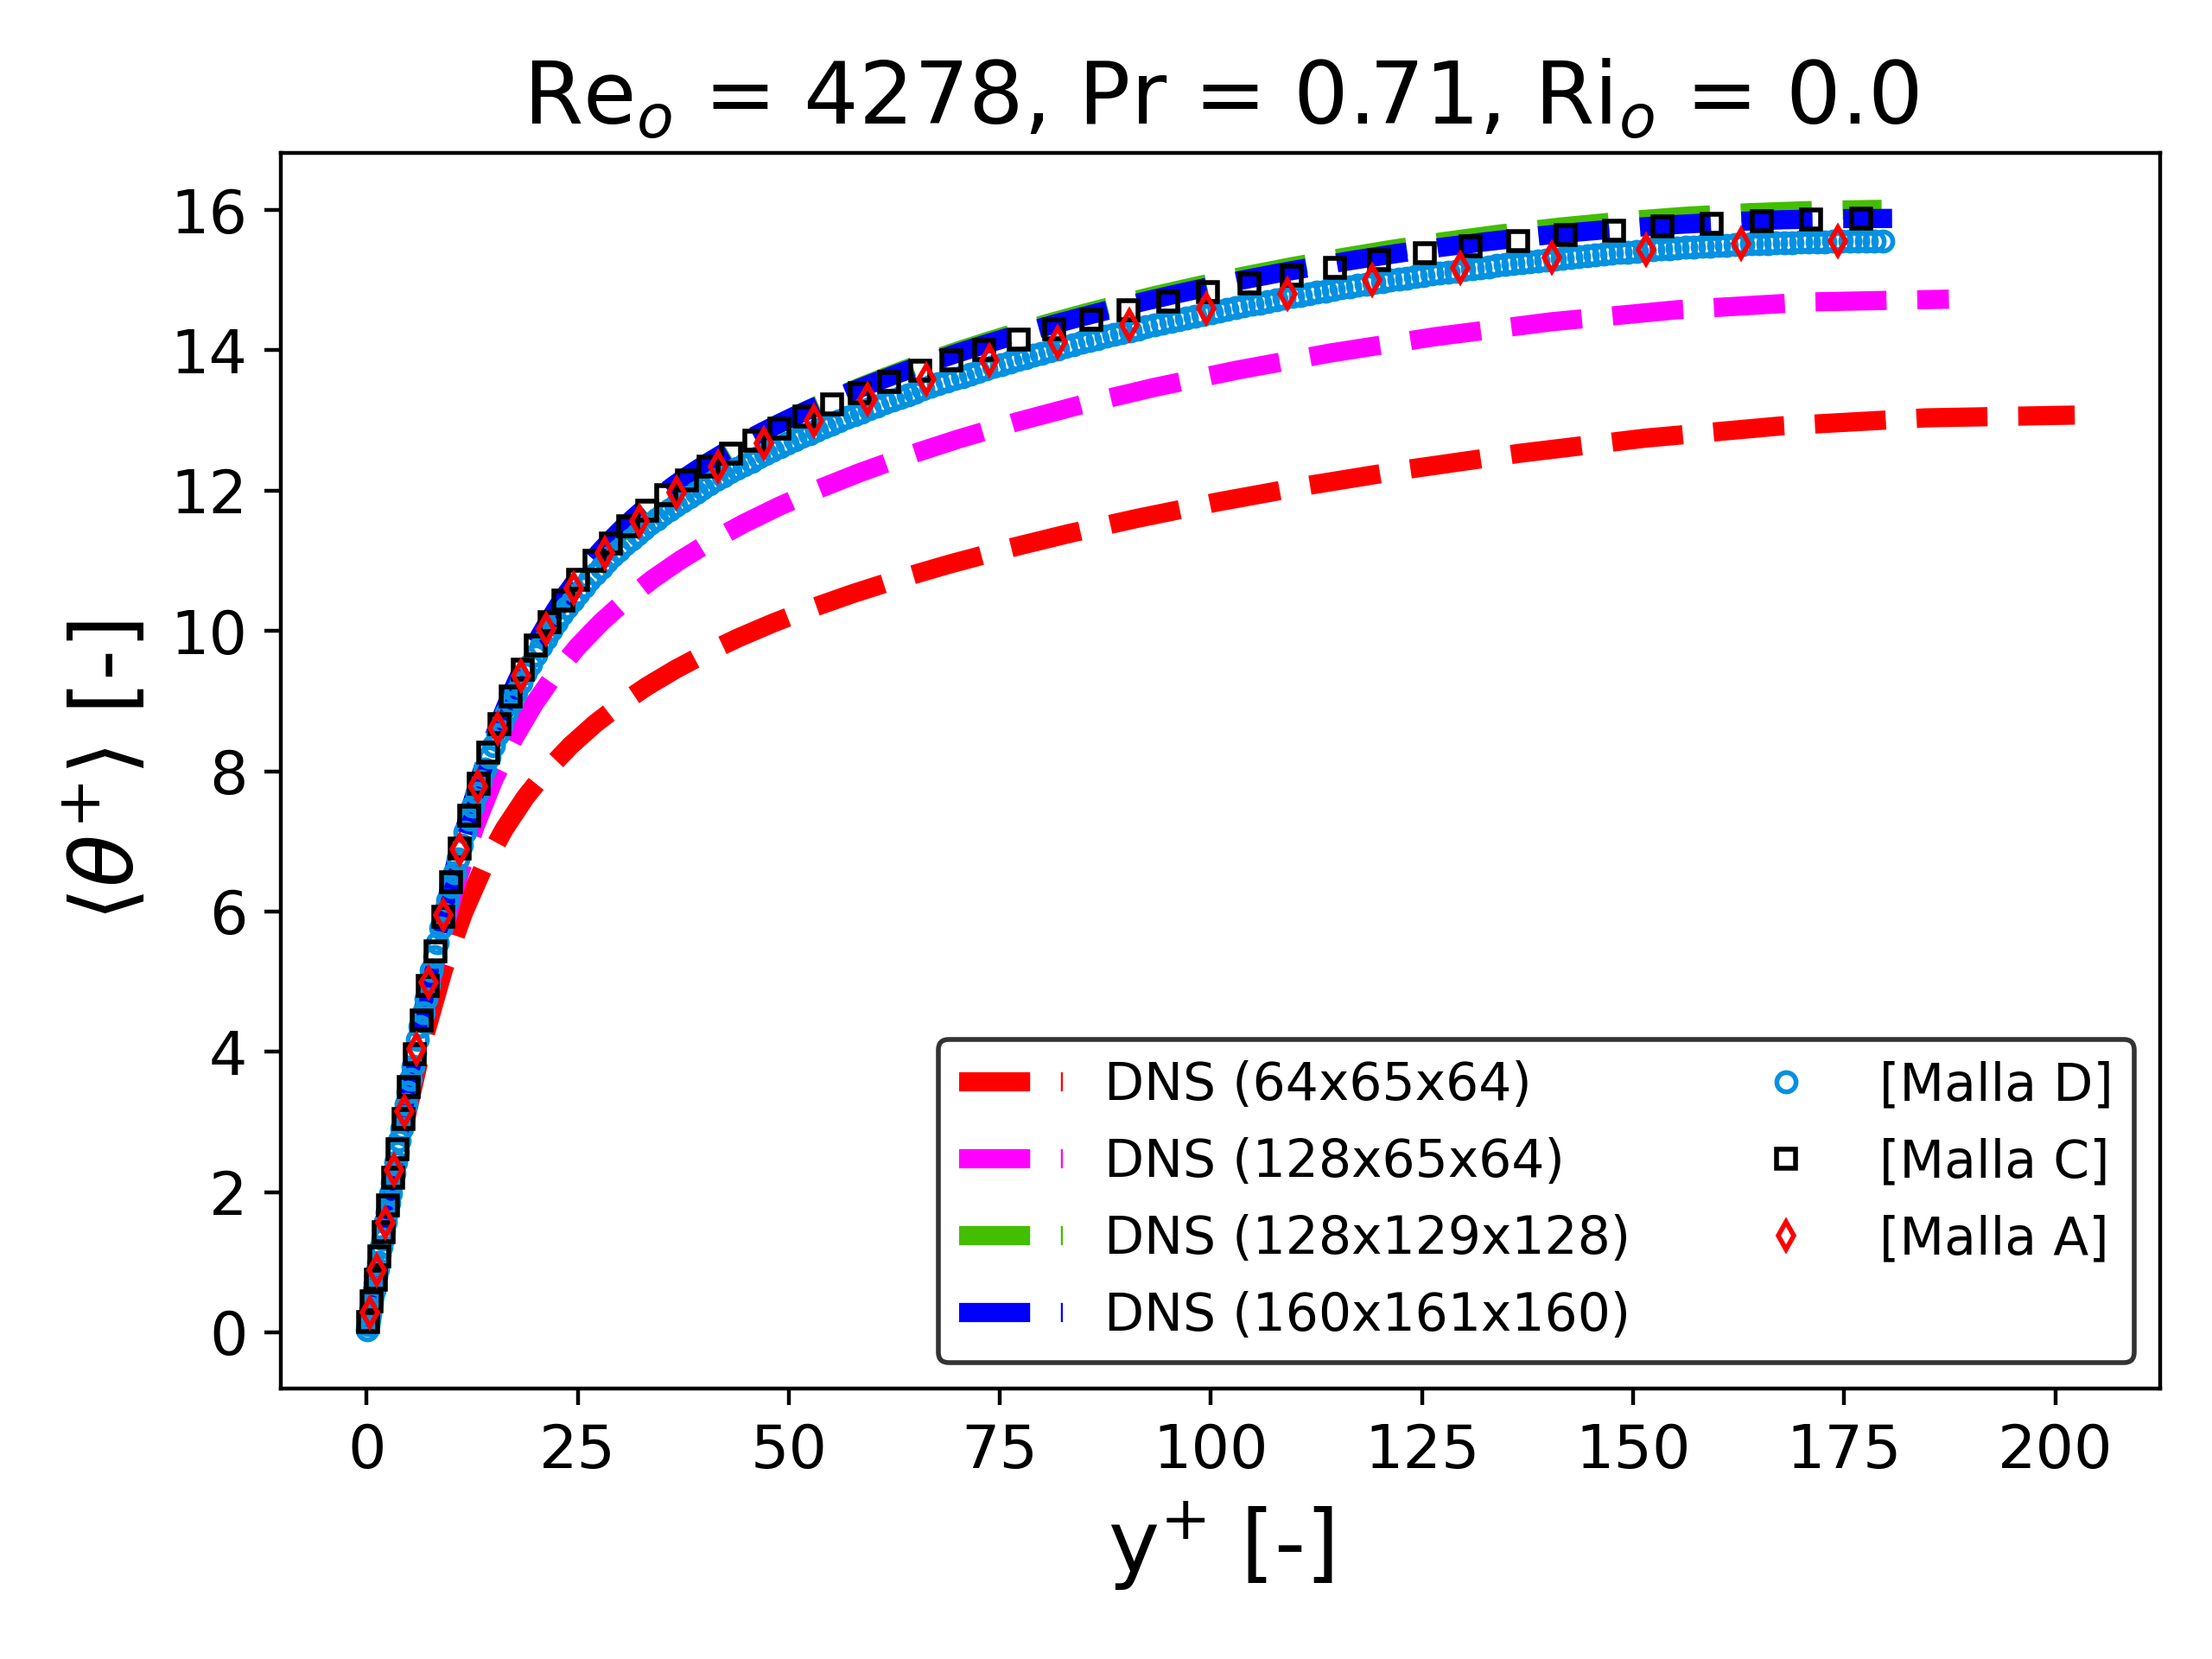
\includegraphics[width=0.49\textwidth]{results/kawamura/meshes/tep_theta.png}
    \label{fig:phi_mean_kawa}}  
    \subfloat[]{
    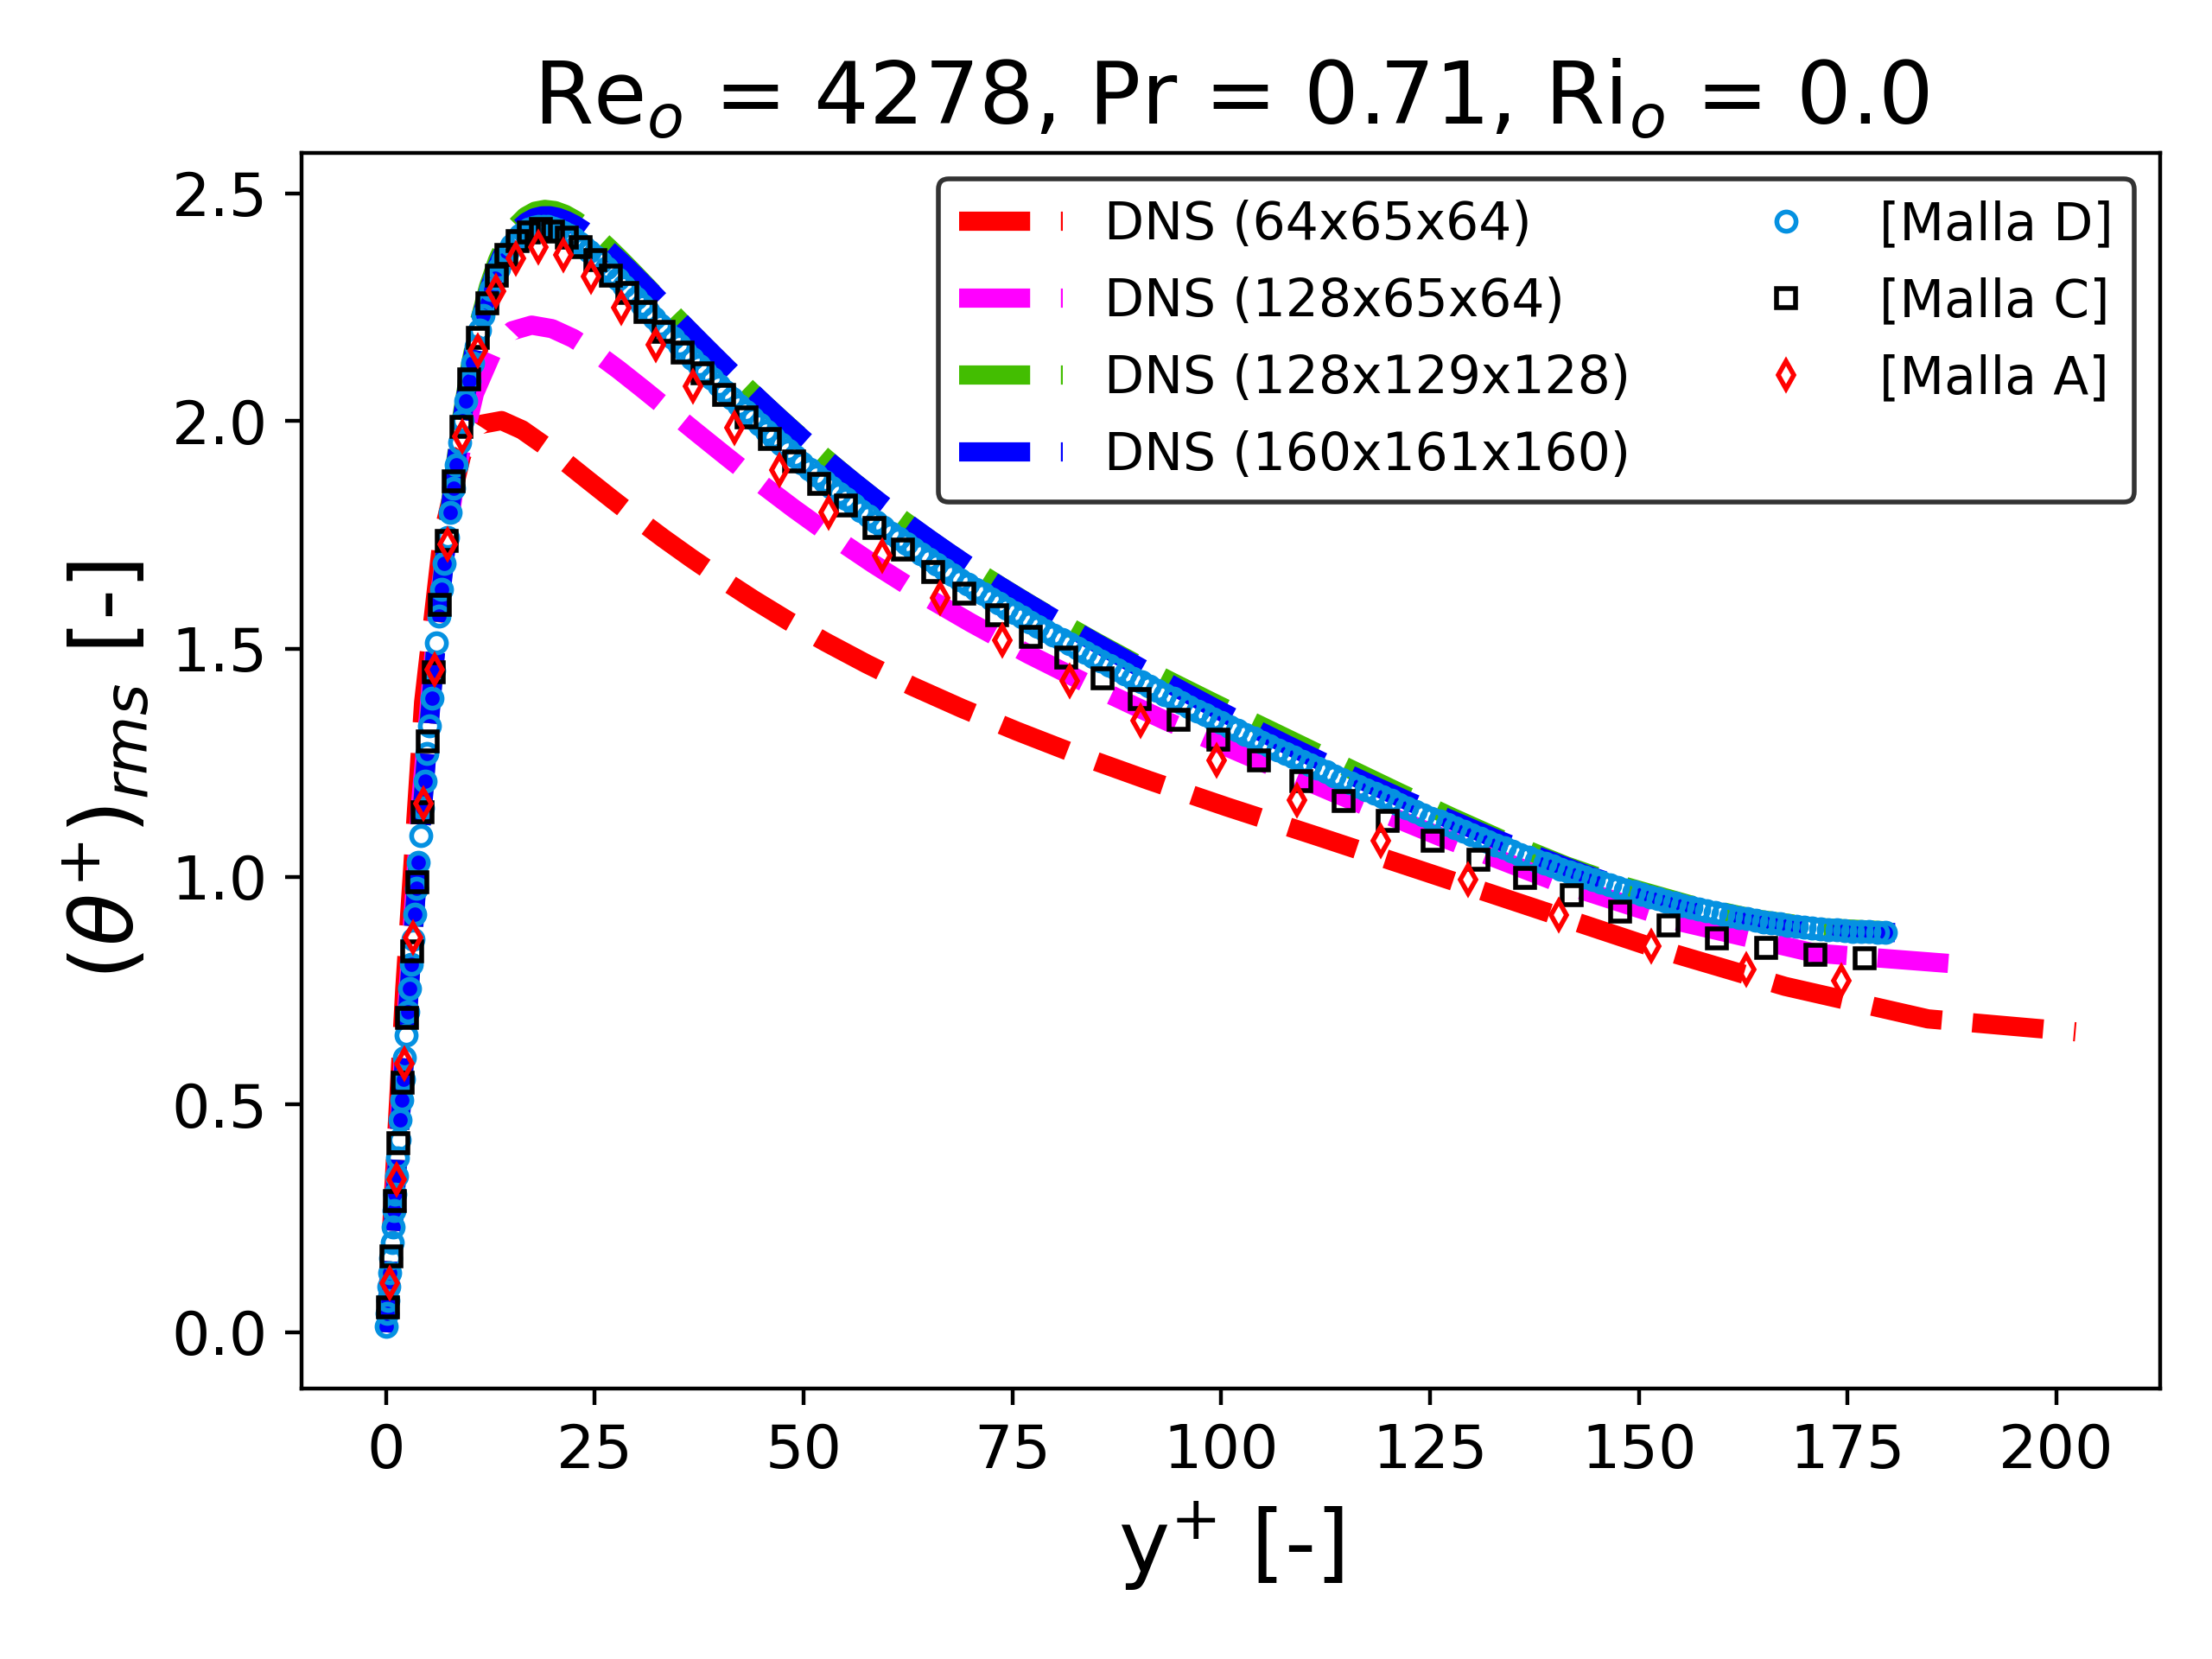
\includegraphics[width=0.49\textwidth]{results/kawamura/meshes/tep_thetap_rms.png}
    \label{fig:phi_rms_kawa}}  
 \caption{a) Perfiles de temperatura media $\langle  \theta^+ \rangle$ en unidades de pared. b) Fluctuaciones de la temperatura.} 
 \label{fig:kawamura_3}
\end{figure}


\begin{figure}[H]
 \centering
  \subfloat[]{
    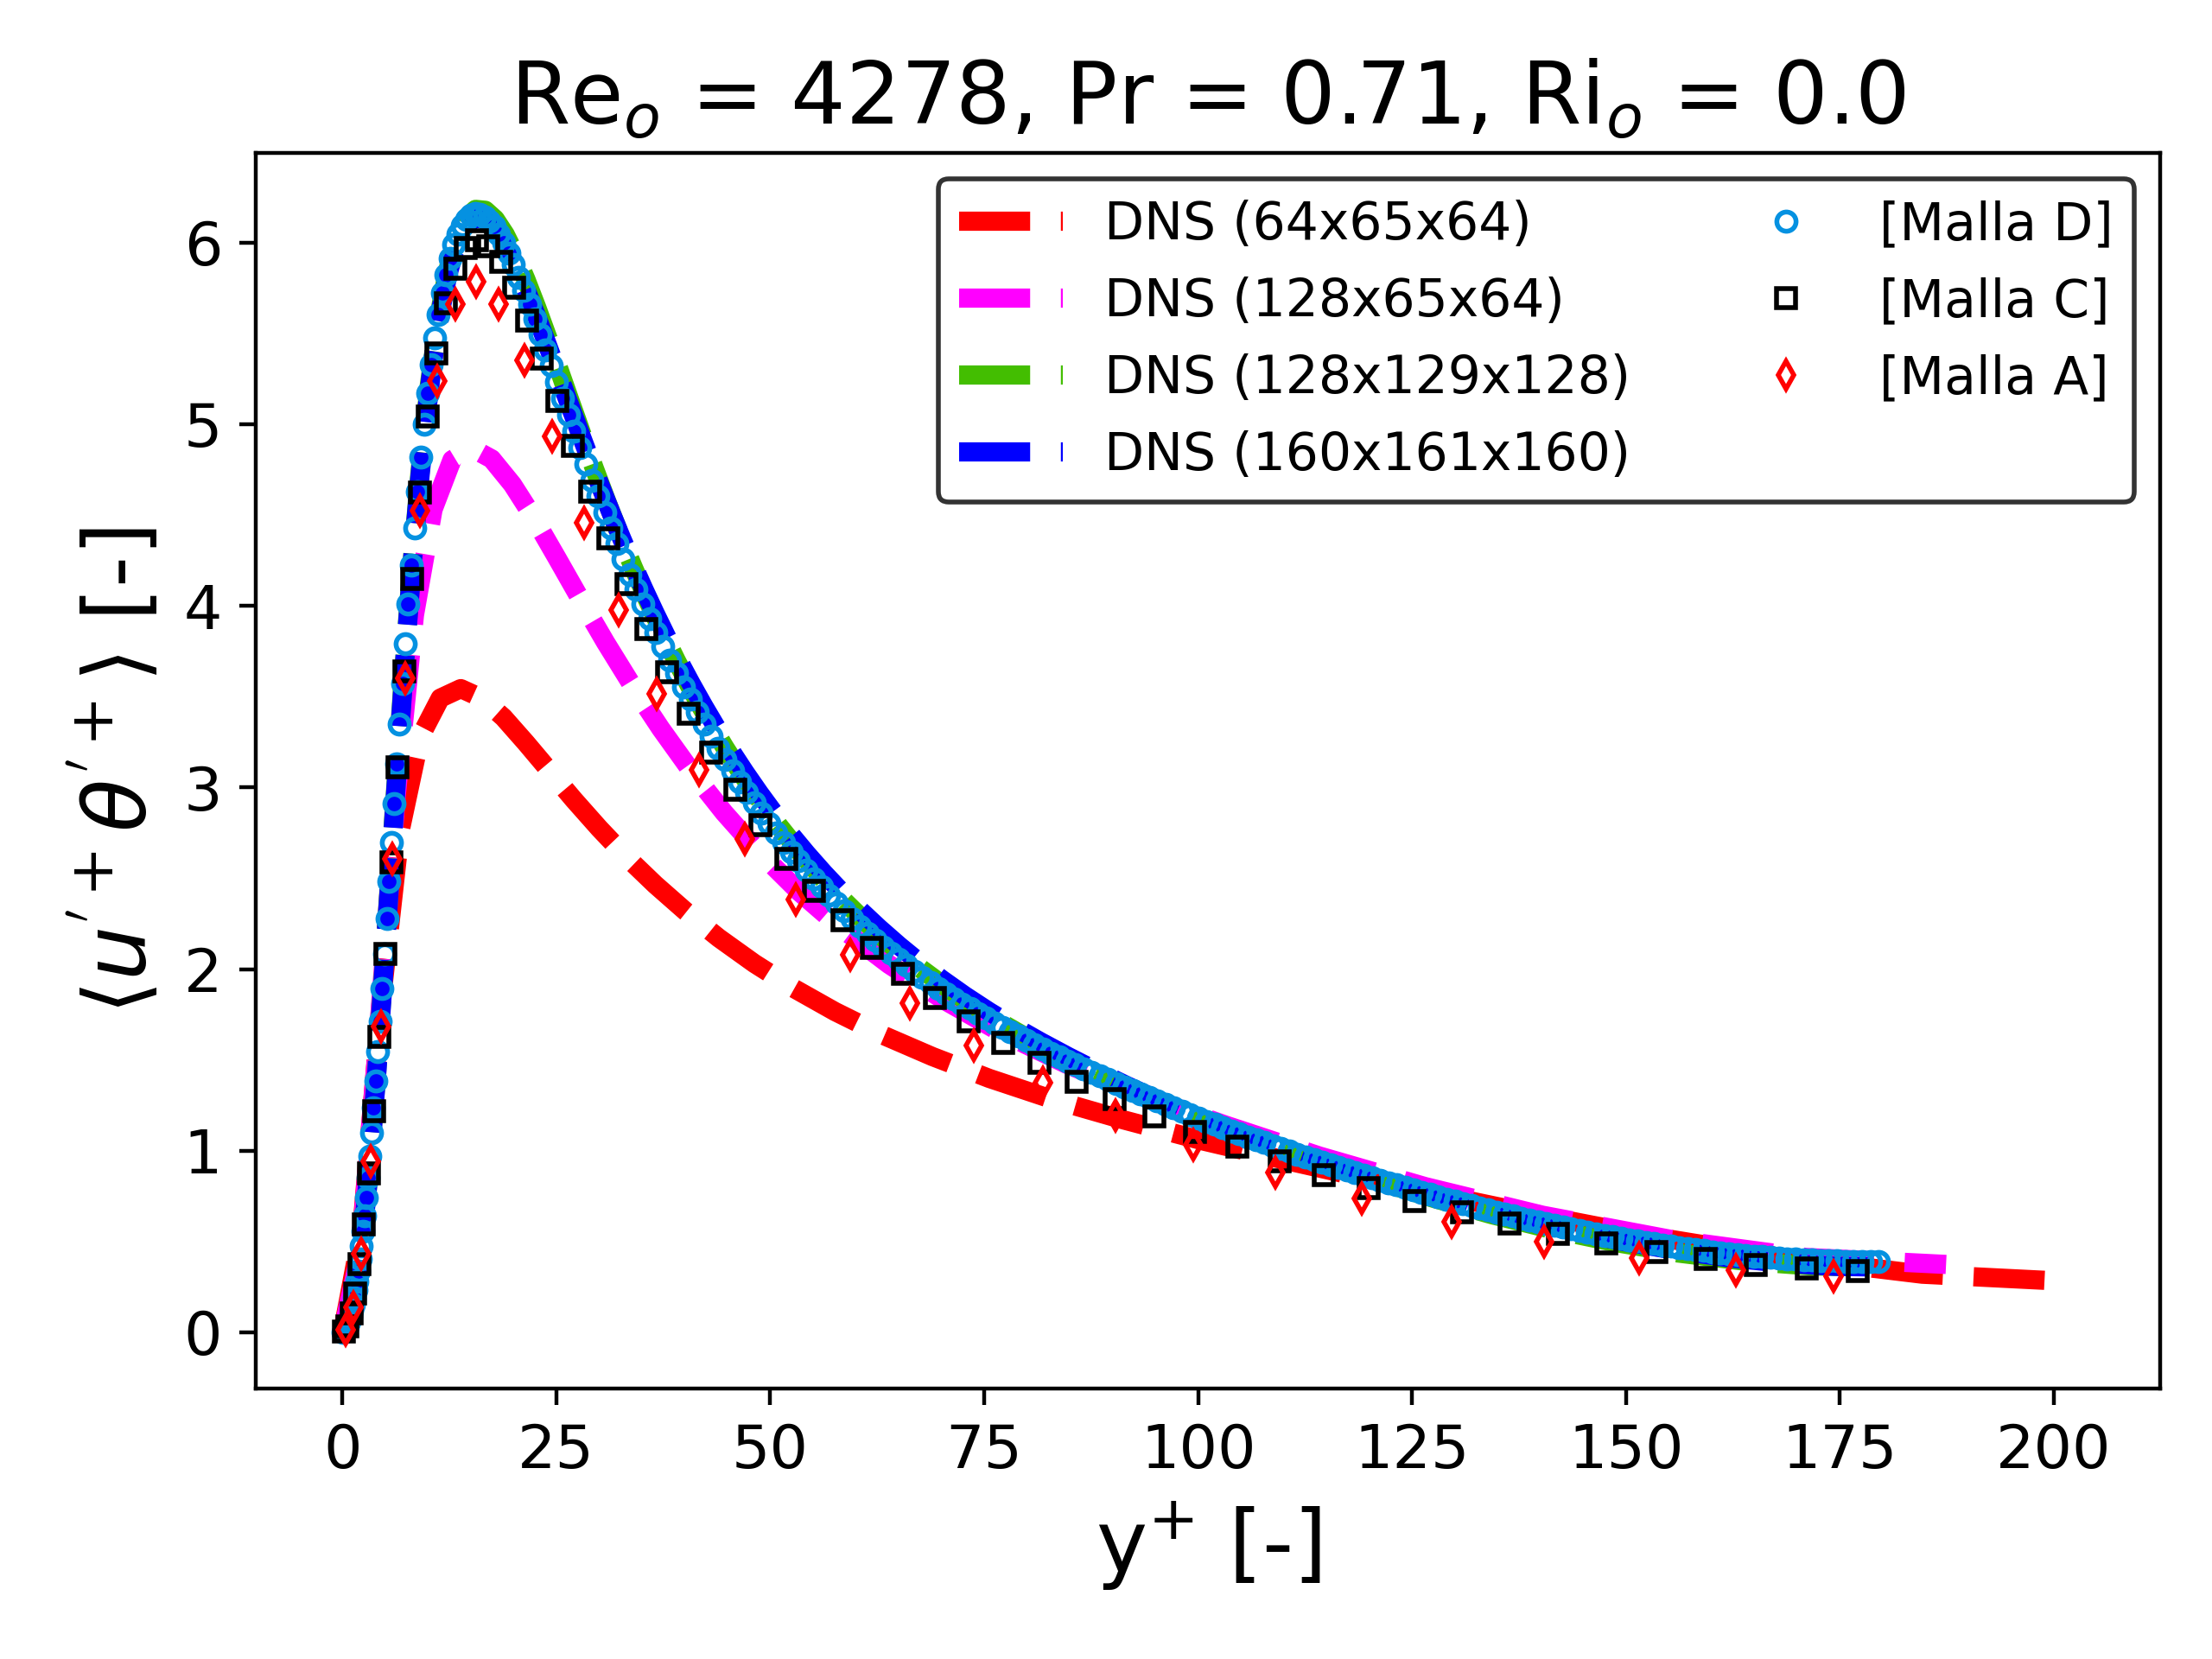
\includegraphics[width=0.49\textwidth]{results/kawamura/meshes/tep_up_thetap.png}
    \label{fig:phi_up_thetap_kawa}}
  \subfloat[]{
    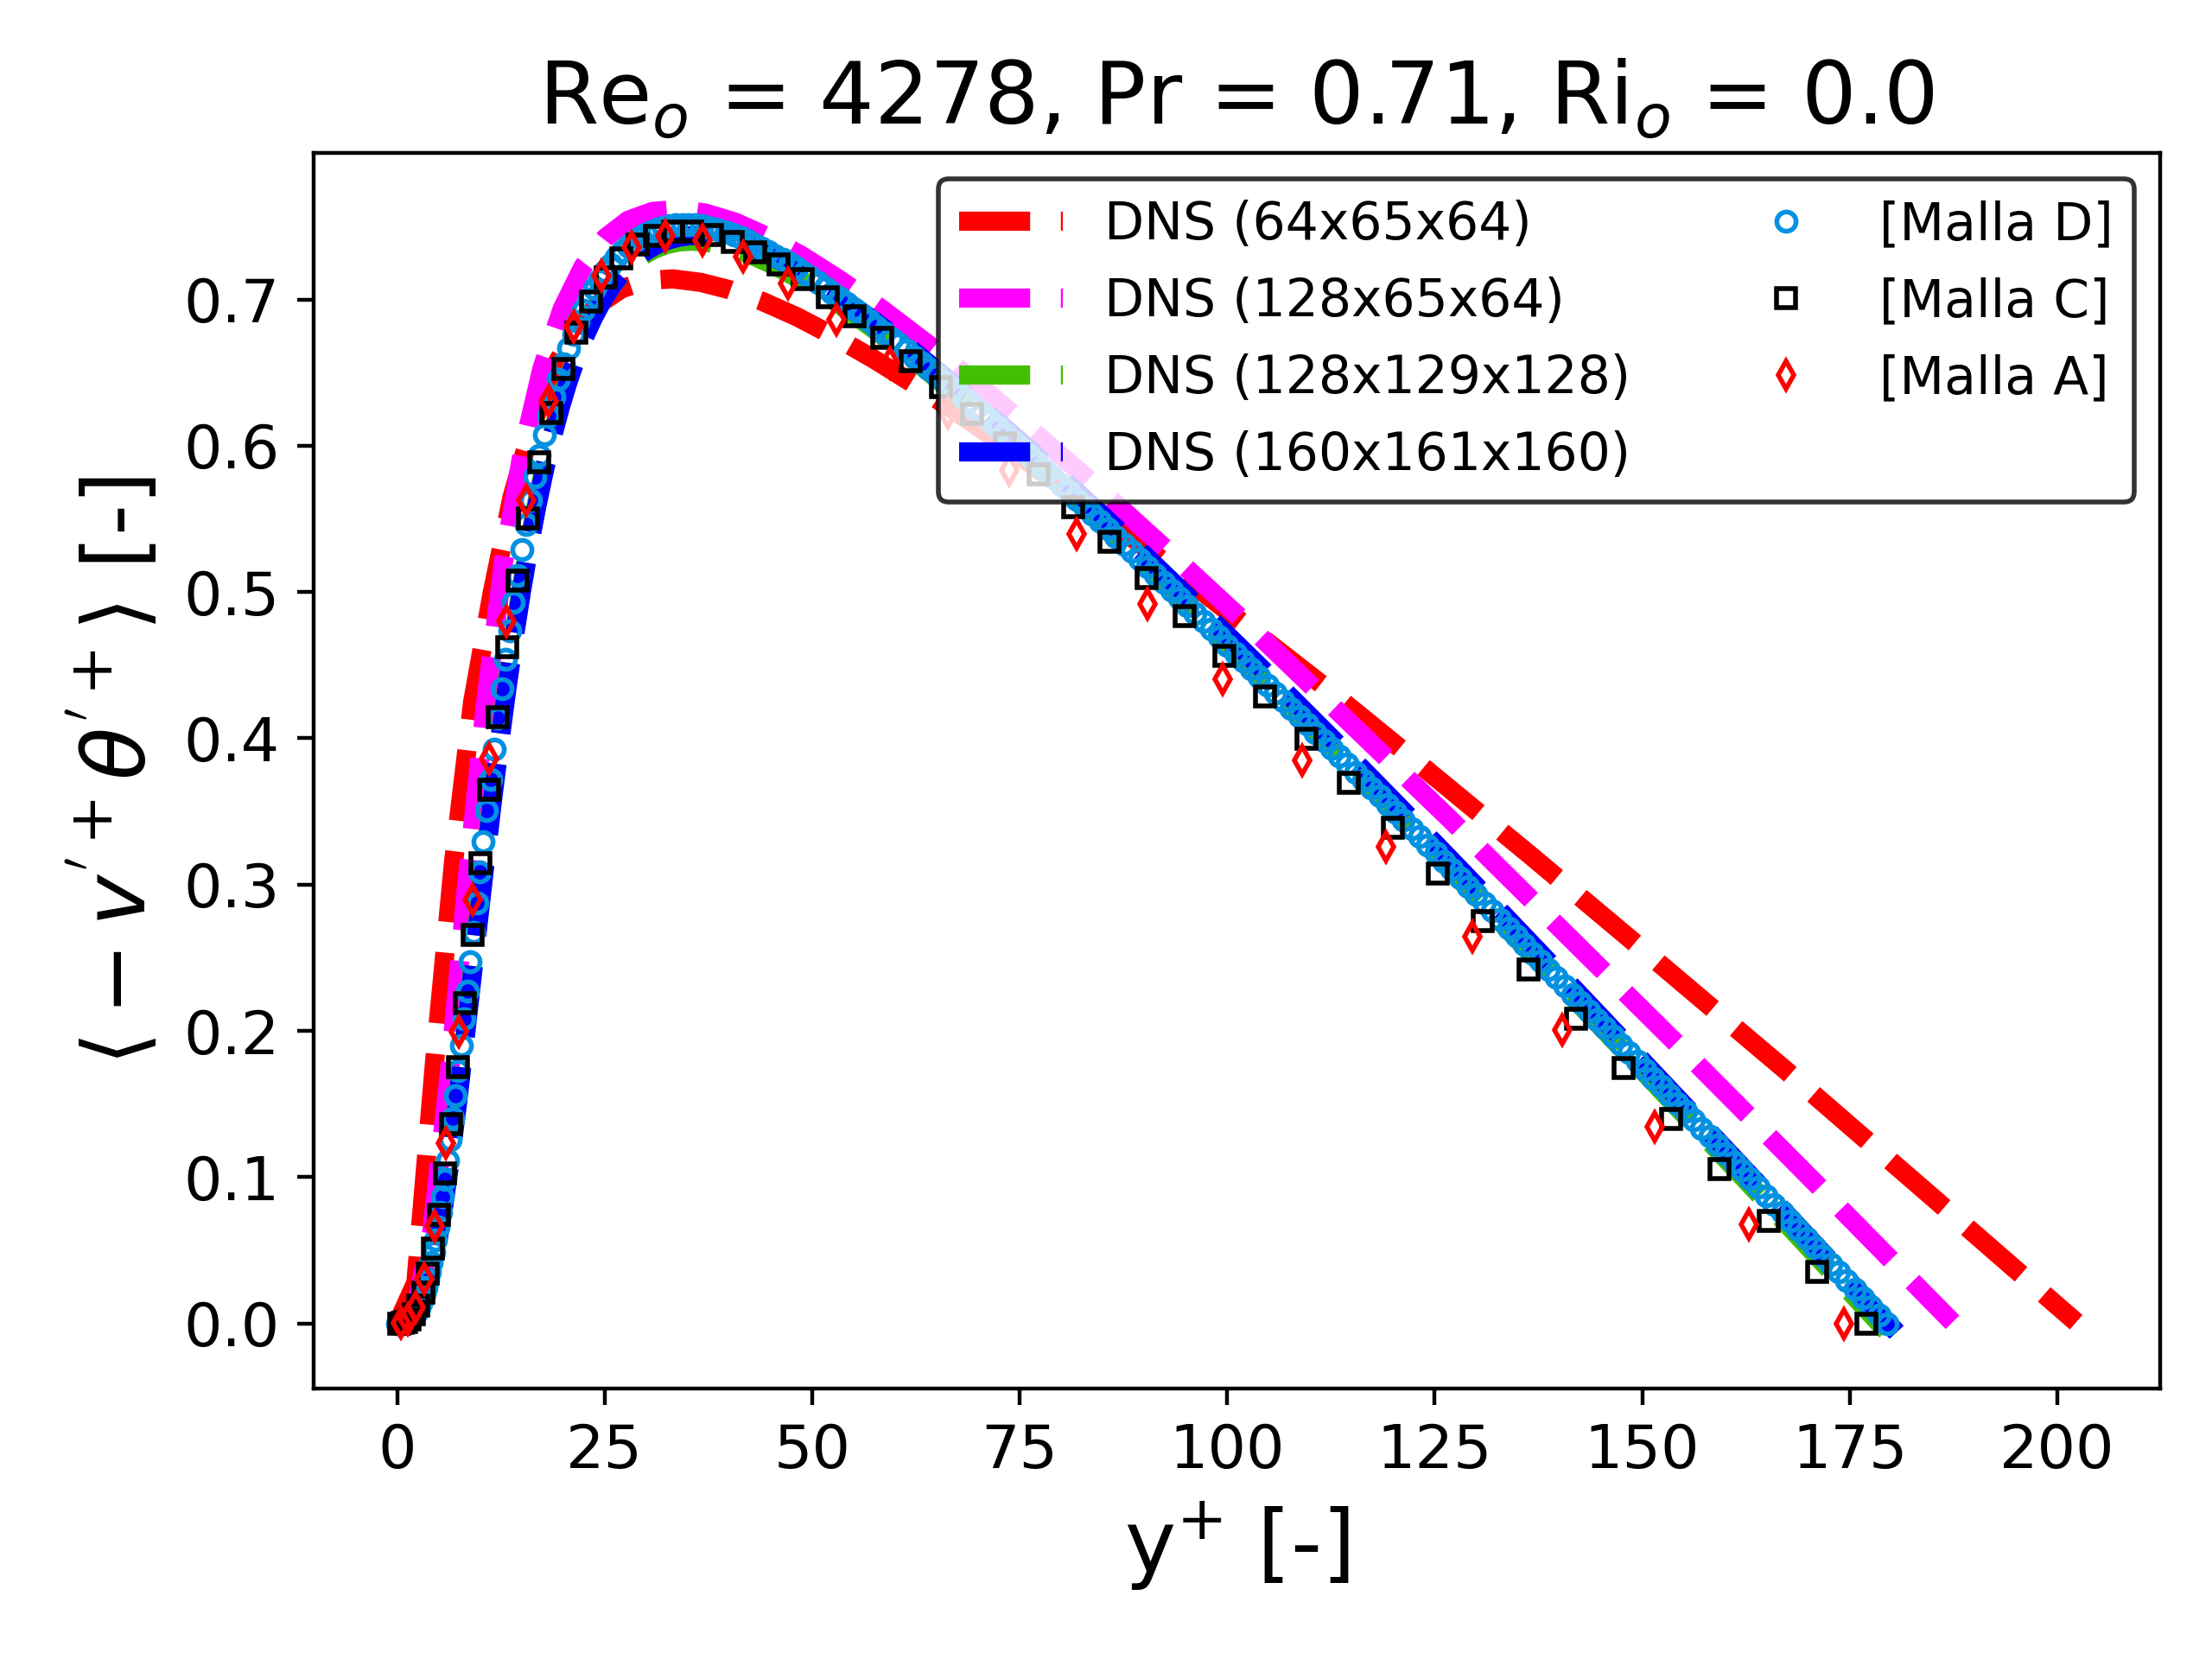
\includegraphics[width=0.49\textwidth]{results/kawamura/meshes/tep_vp_thetap.png}
    \label{fig:phi_vp_thetap_kawa}}  
    
   \caption{a) Flujo turbulento de calor en la dirección X. b) Flujo turbulento de calor en la dirección Y.} 
 \label{fig:kawamura_4}
\end{figure}


\section{Validación de Simulaciones de Canales Periódicos con Convección Mixta}

\subsection{Caso $\mathbf{Ri_b}=0.5$}

\begin{figure}[H]
 \centering

  \subfloat[]{
    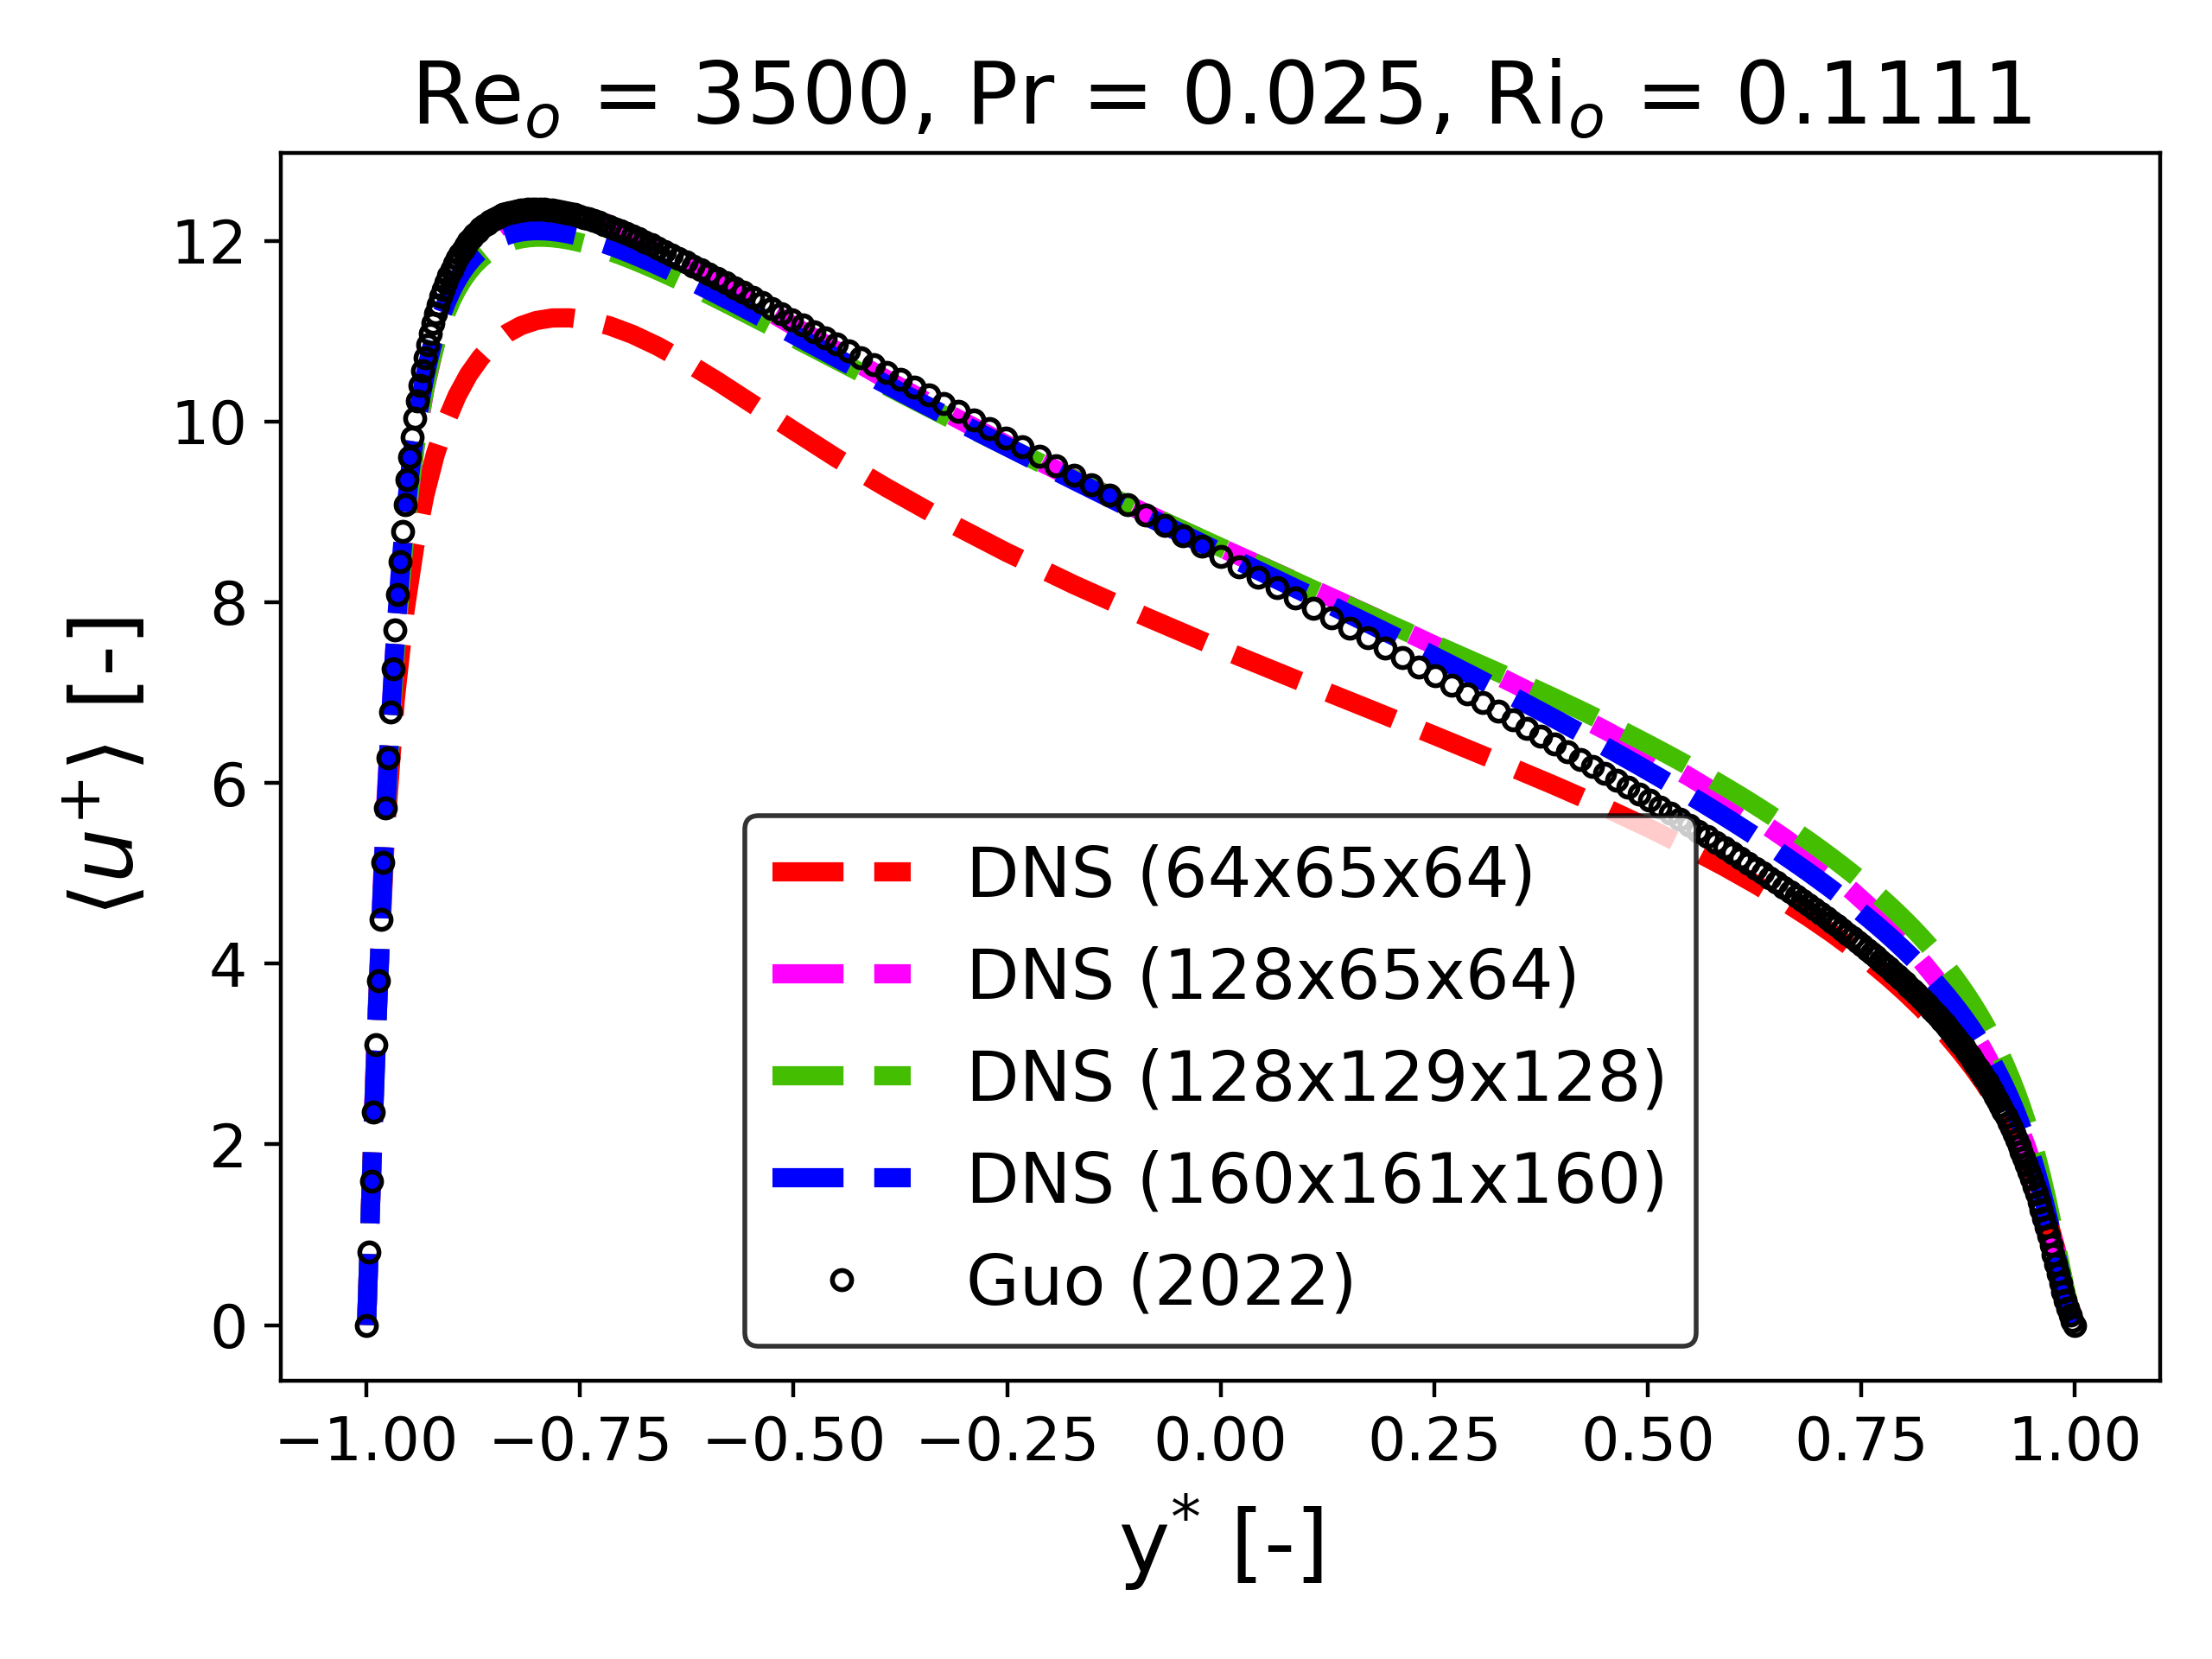
\includegraphics[width=0.49\textwidth]{results/guo/rib05/mct_upmean.png}
    \label{fig:phi_mean_guo}}  
  \subfloat[]{
    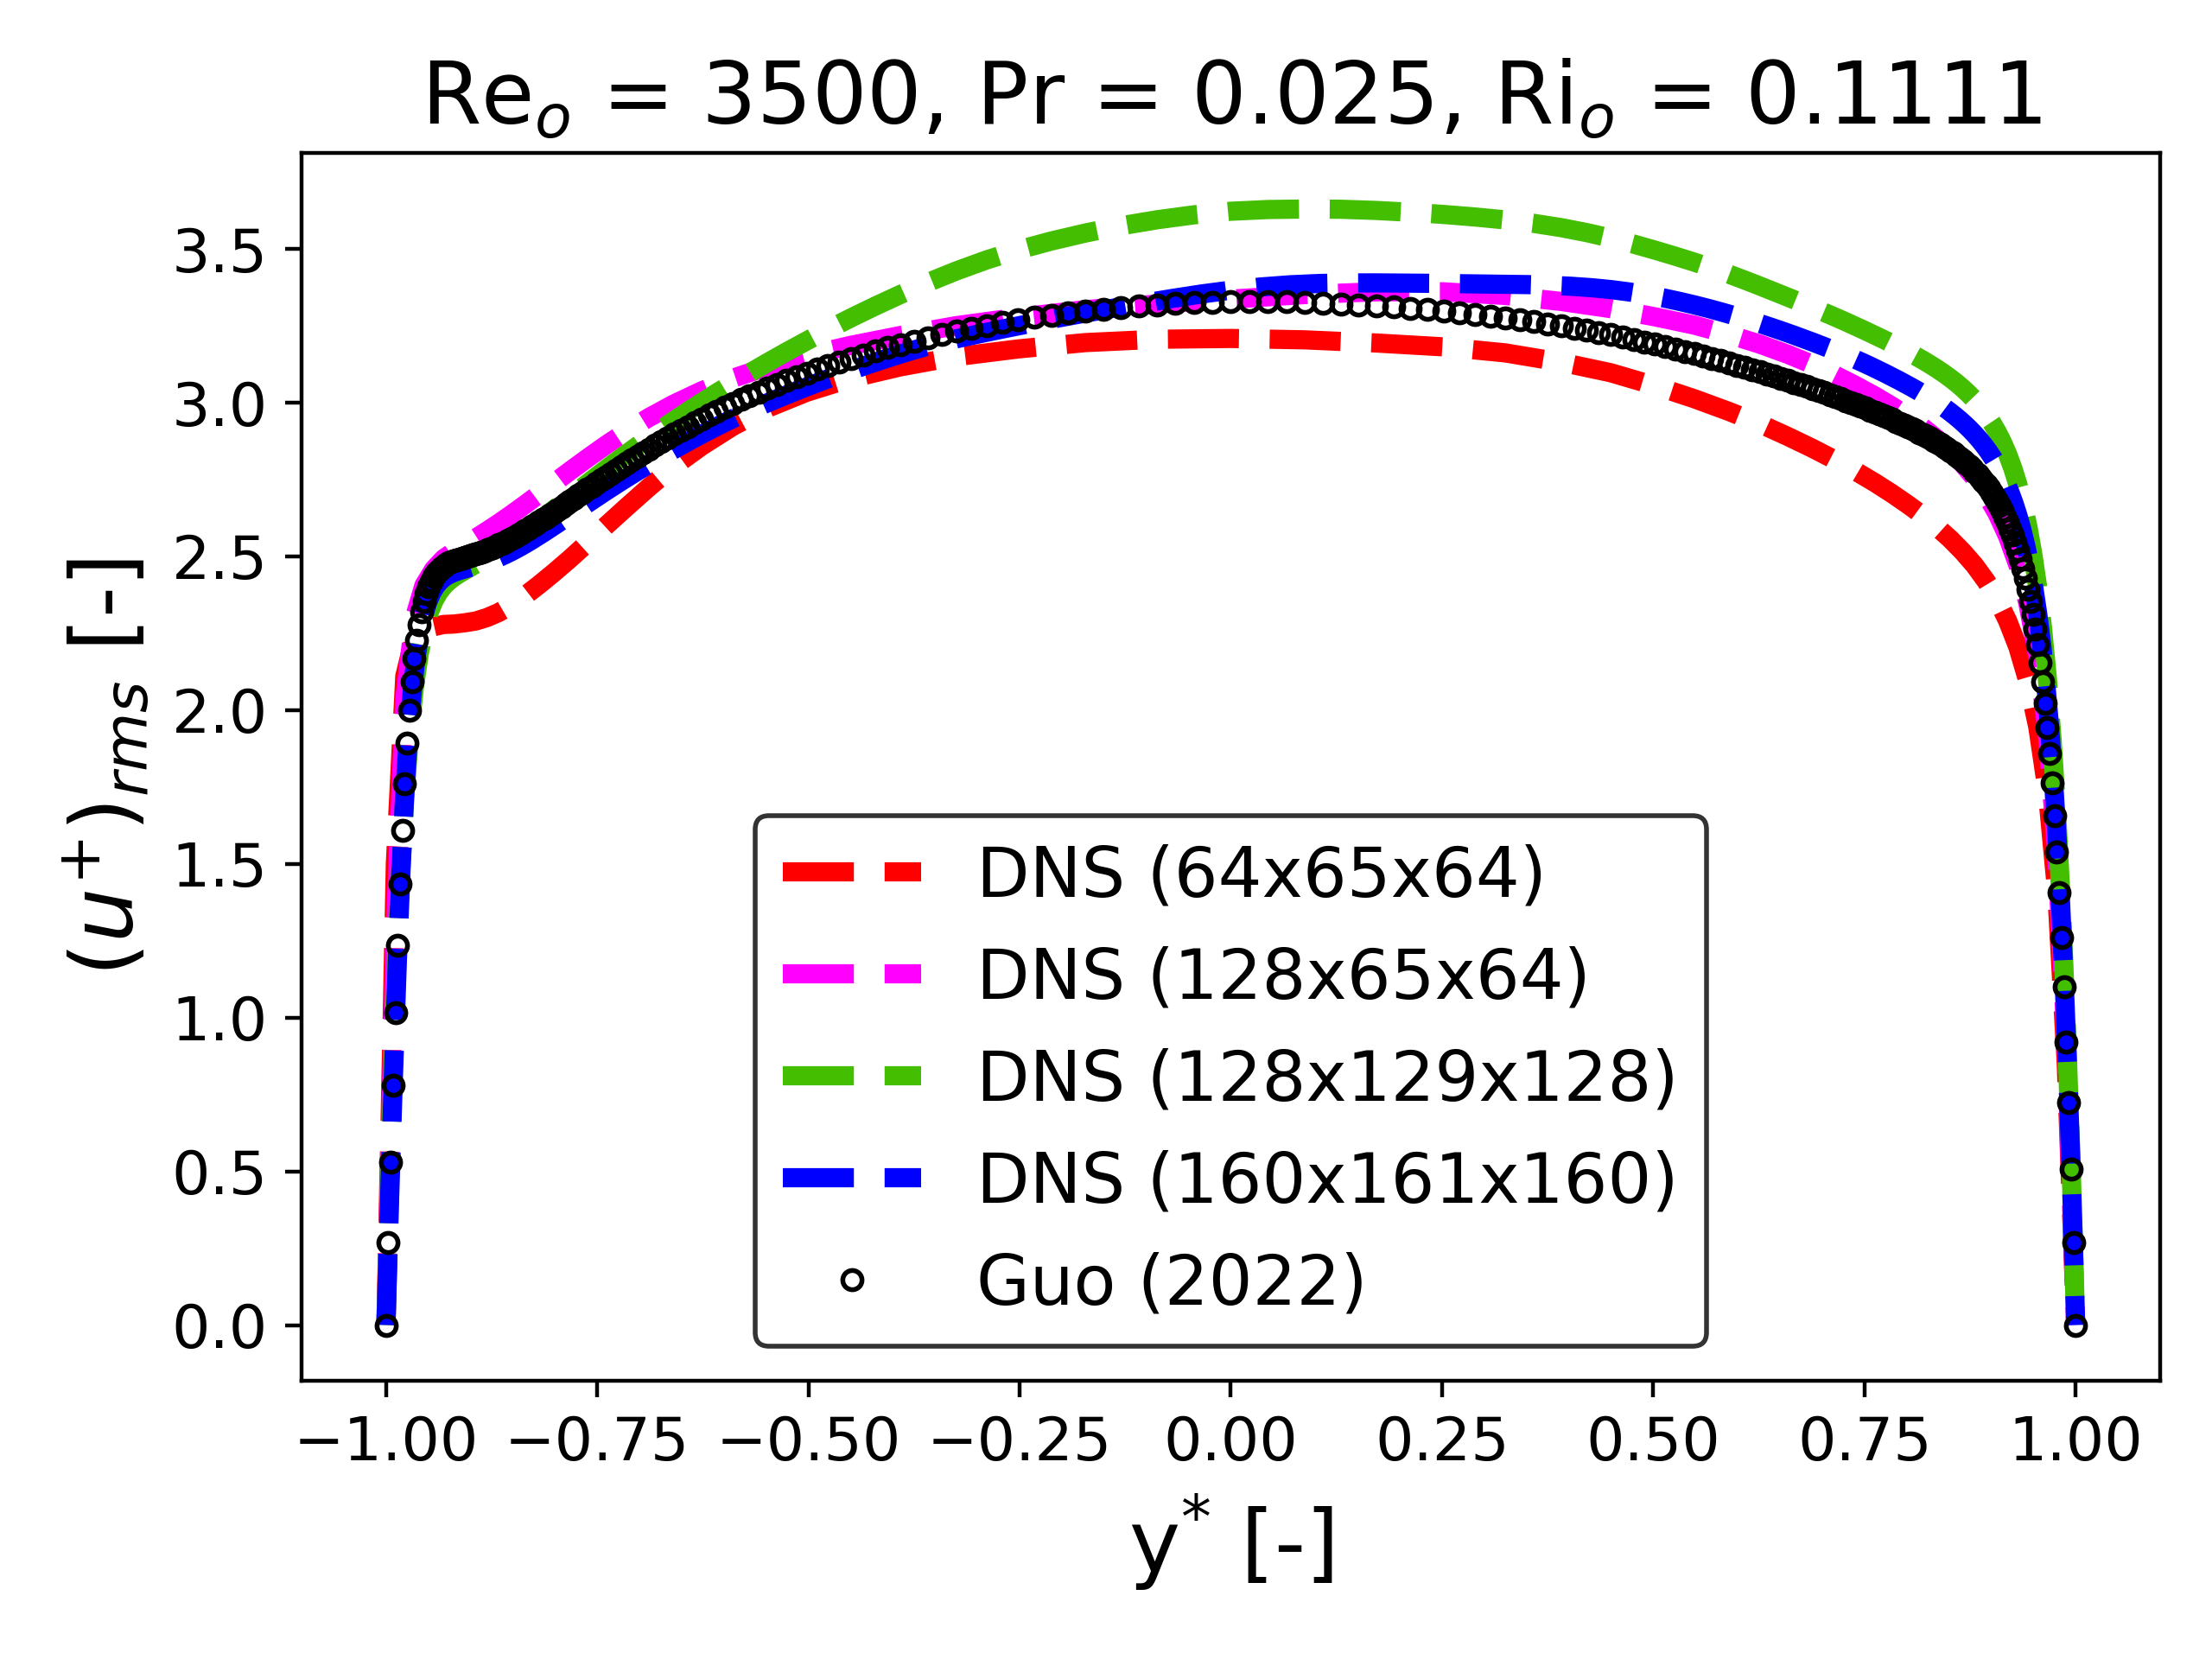
\includegraphics[width=0.49\textwidth]{results/guo/rib05/mct_uprms.png}
    \label{fig:phi_rms_guo}} 
 
  \subfloat[]{
    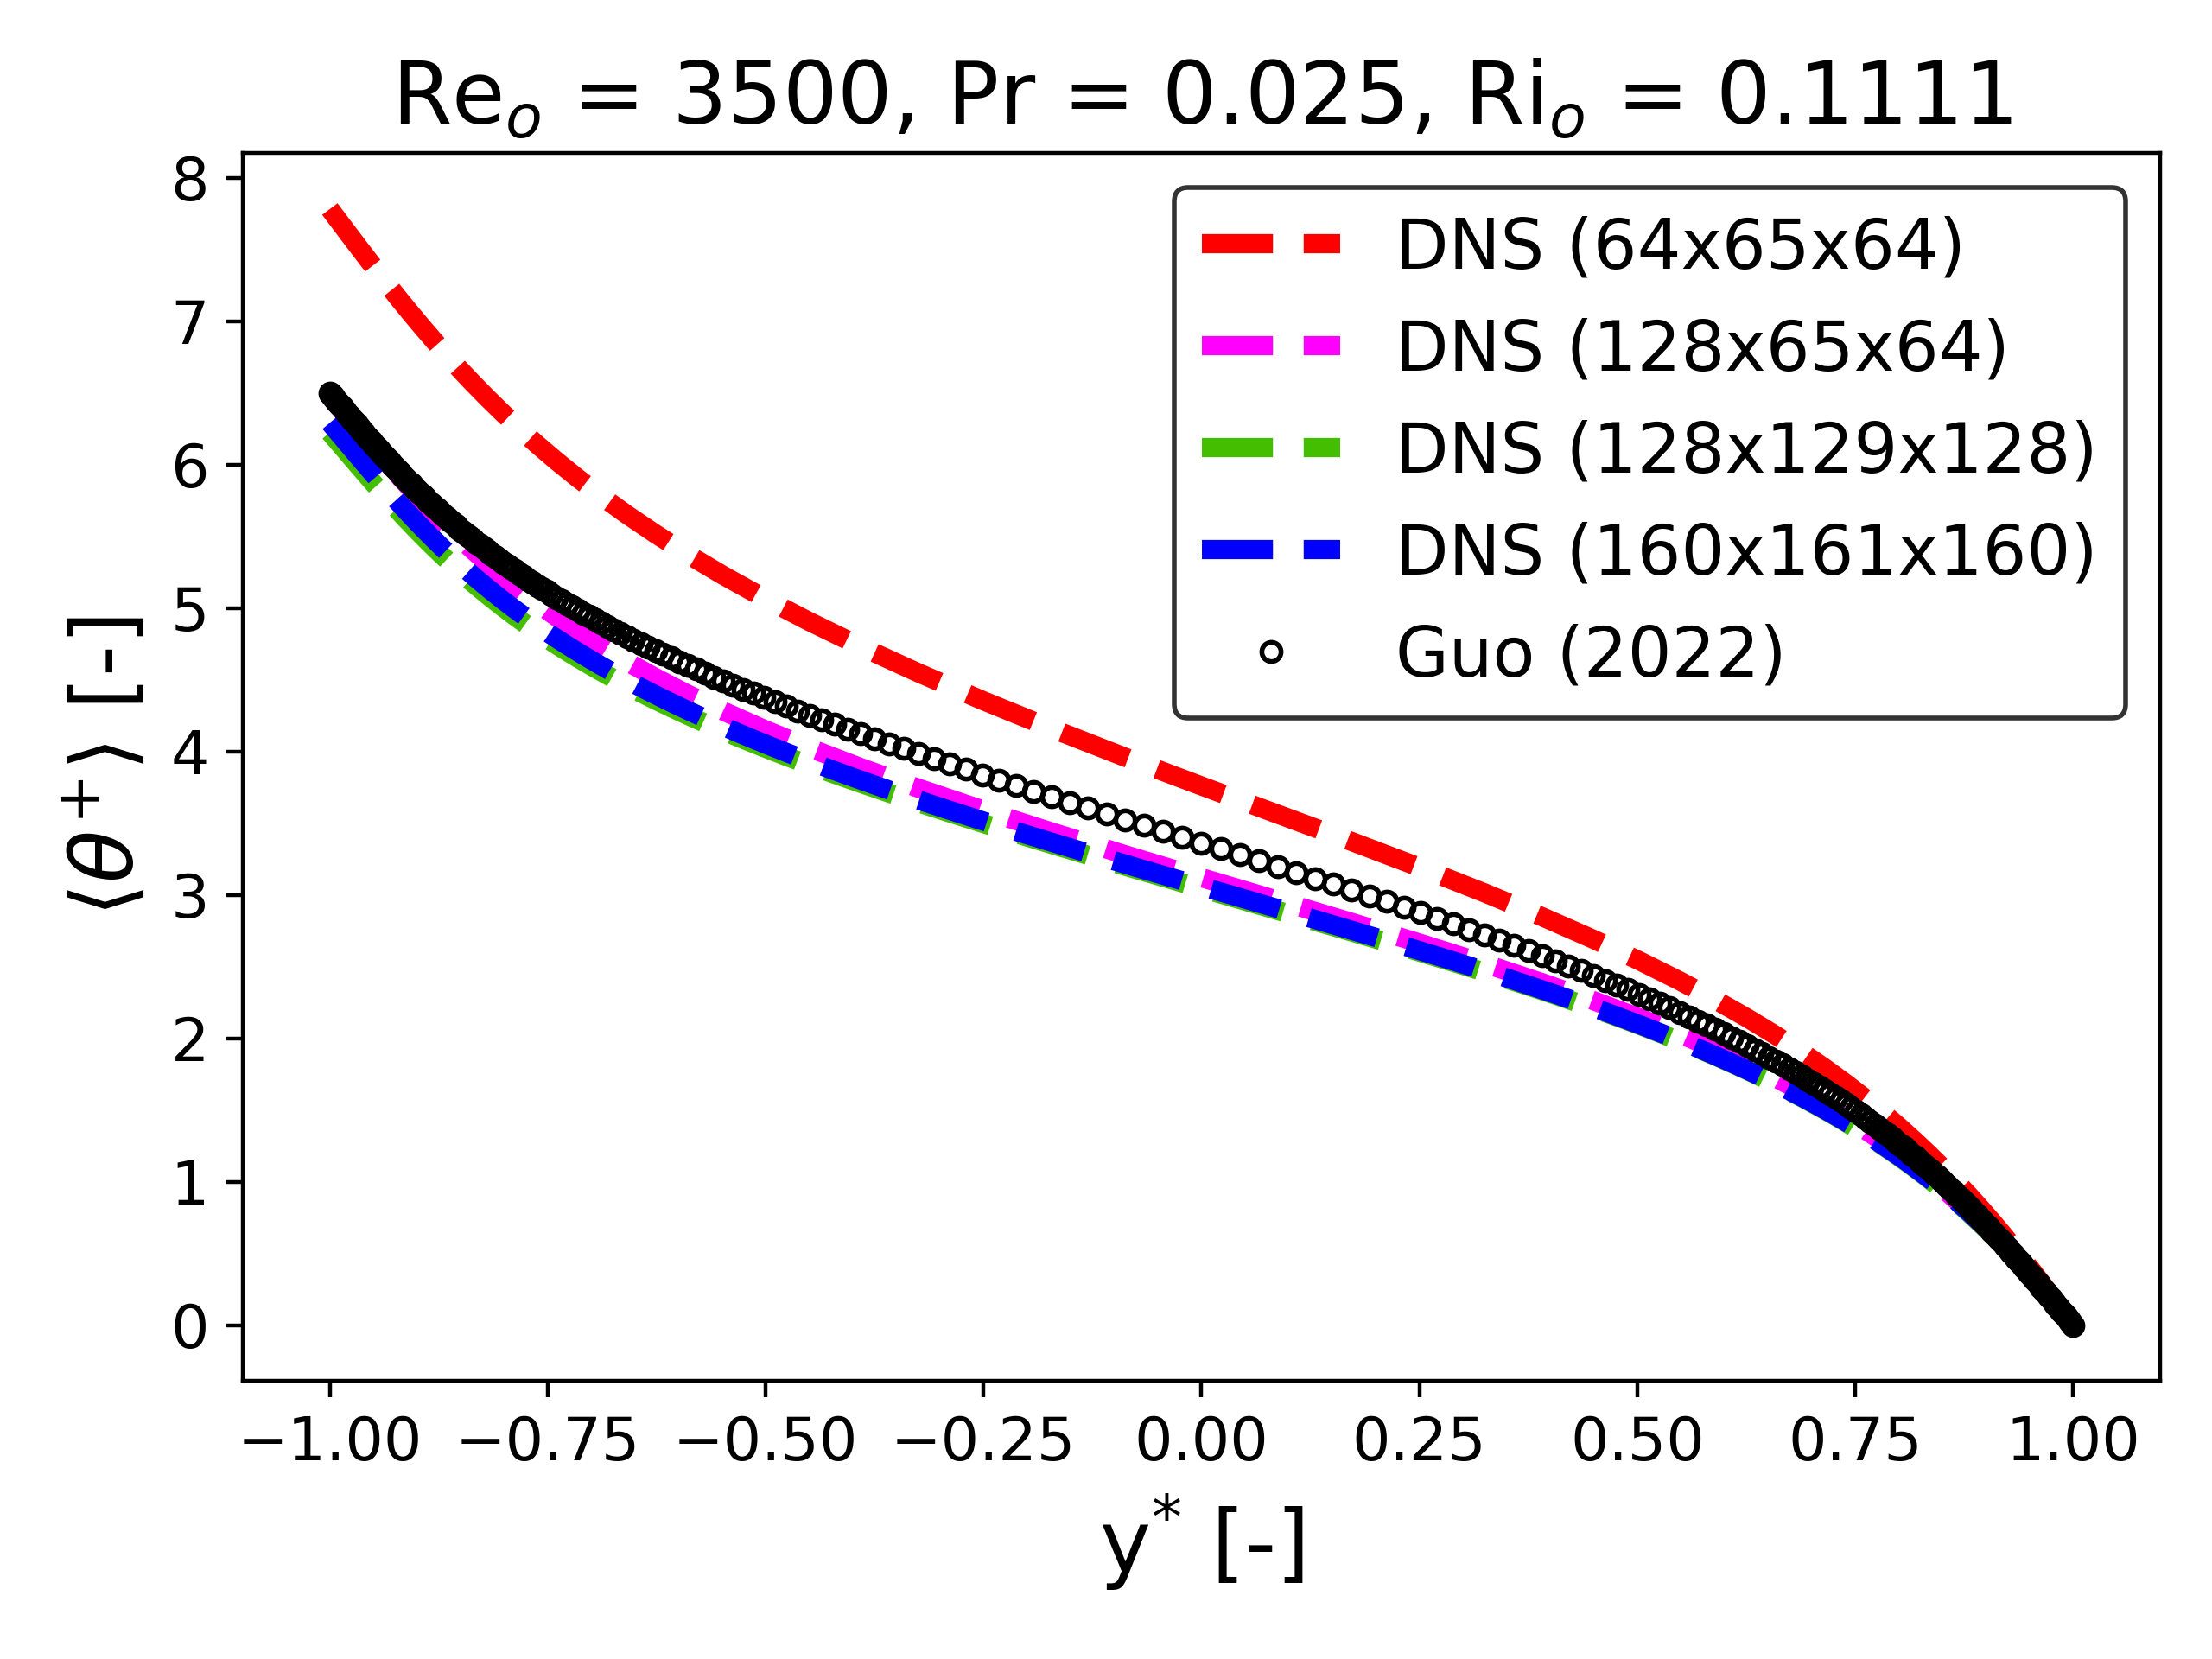
\includegraphics[width=0.49\textwidth]{results/guo/rib05/mct_theta.png}
    \label{fig:phi_mean_guo}}  
  \subfloat[]{
    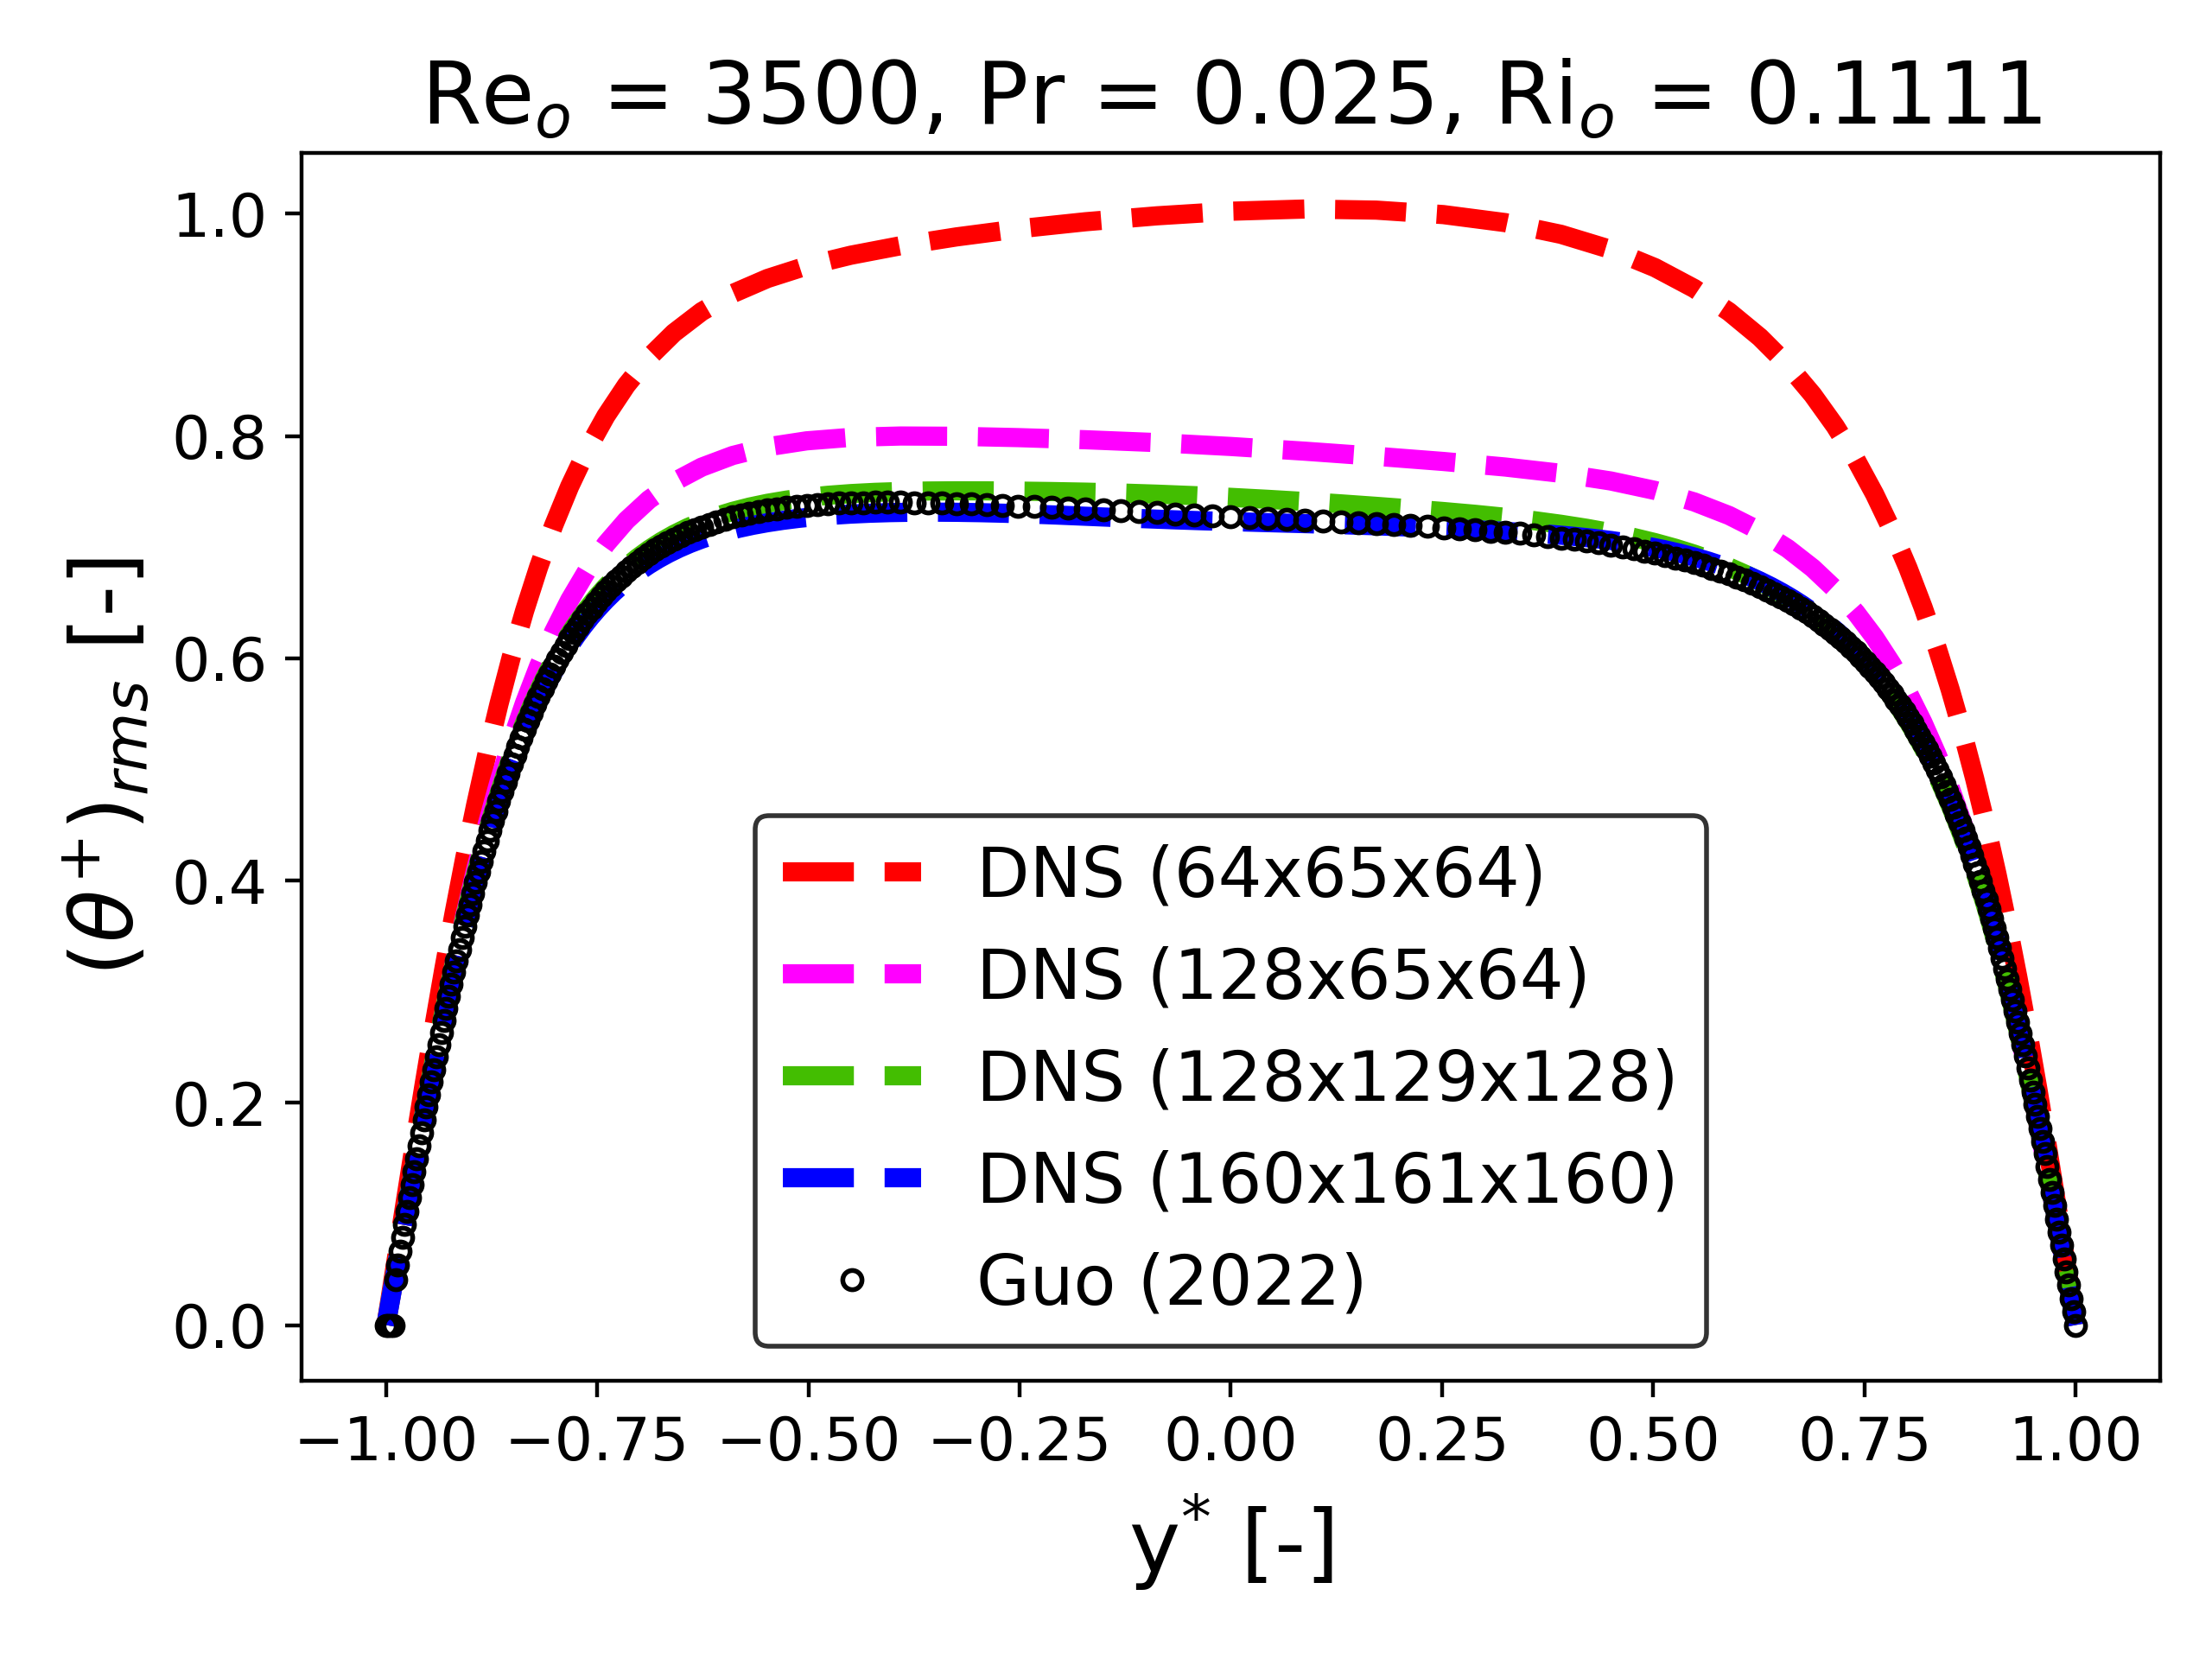
\includegraphics[width=0.49\textwidth]{results/guo/rib05/mct_thetap_rms.png}
    \label{fig:phi_rms_guo}}  

  \subfloat[]{
    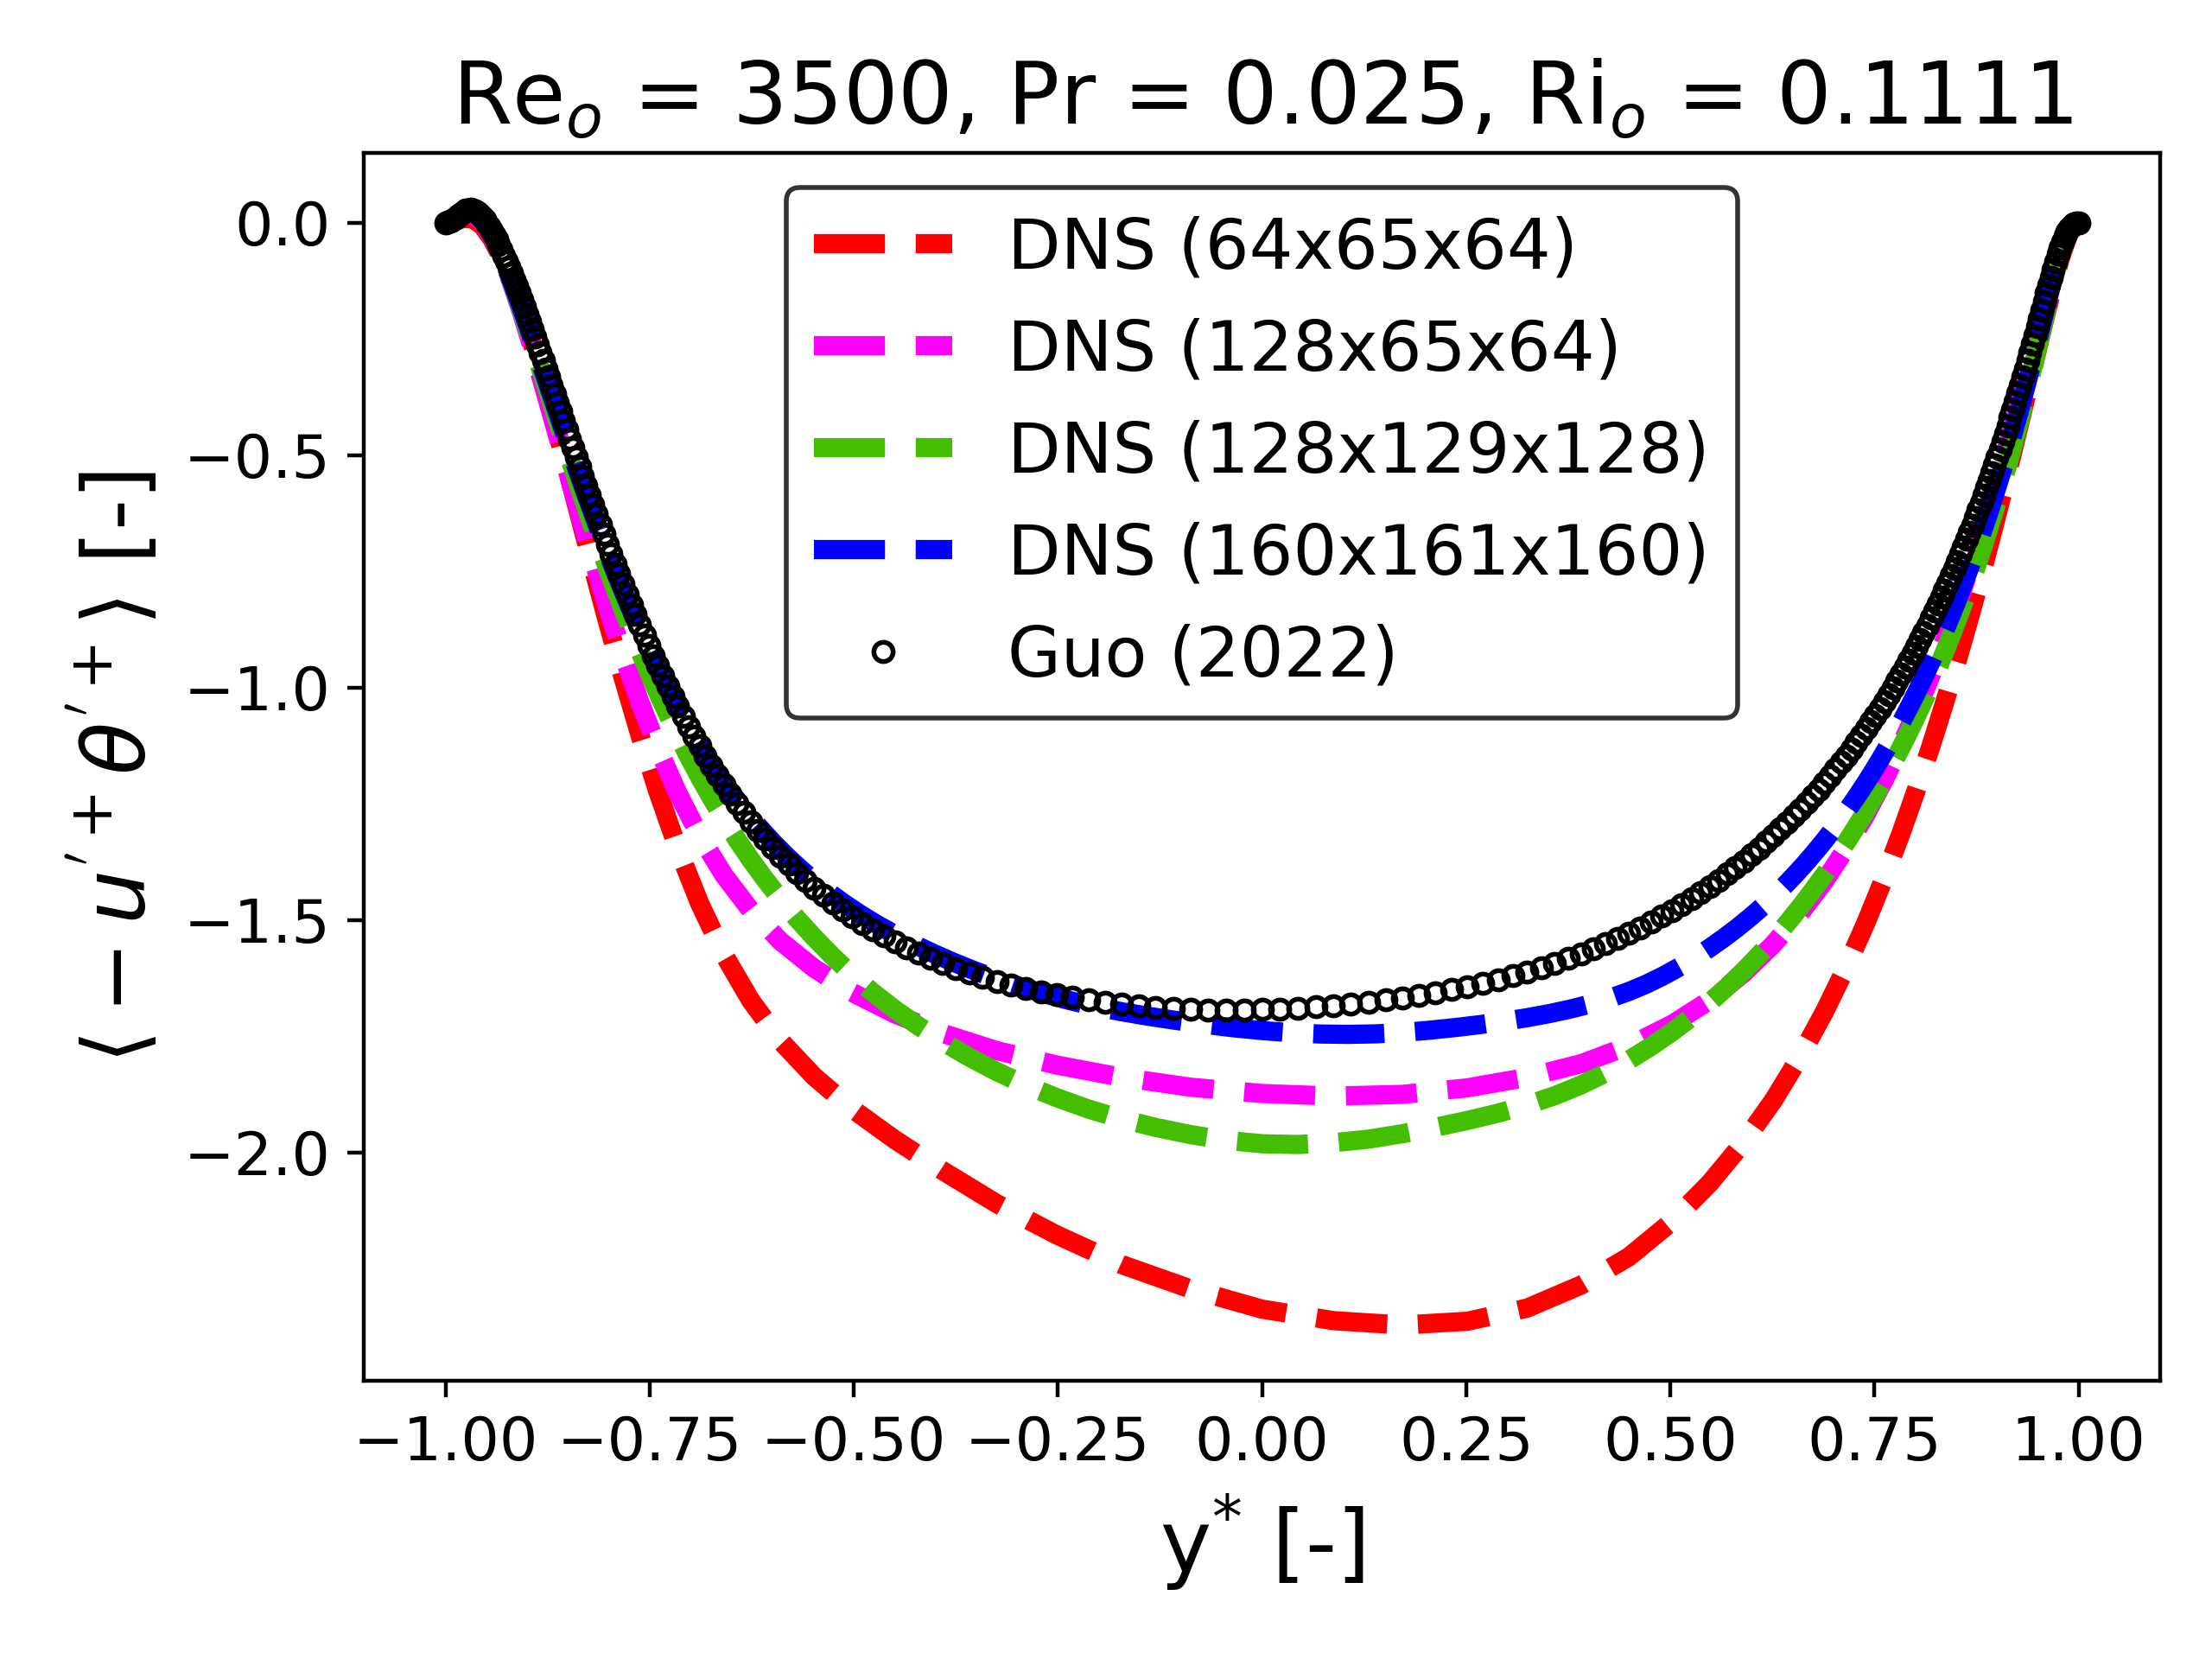
\includegraphics[width=0.49\textwidth]{results/guo/rib05/mct_up_thetap.png}
    \label{fig:phi_up_thetap_guo}}
  \subfloat[]{
    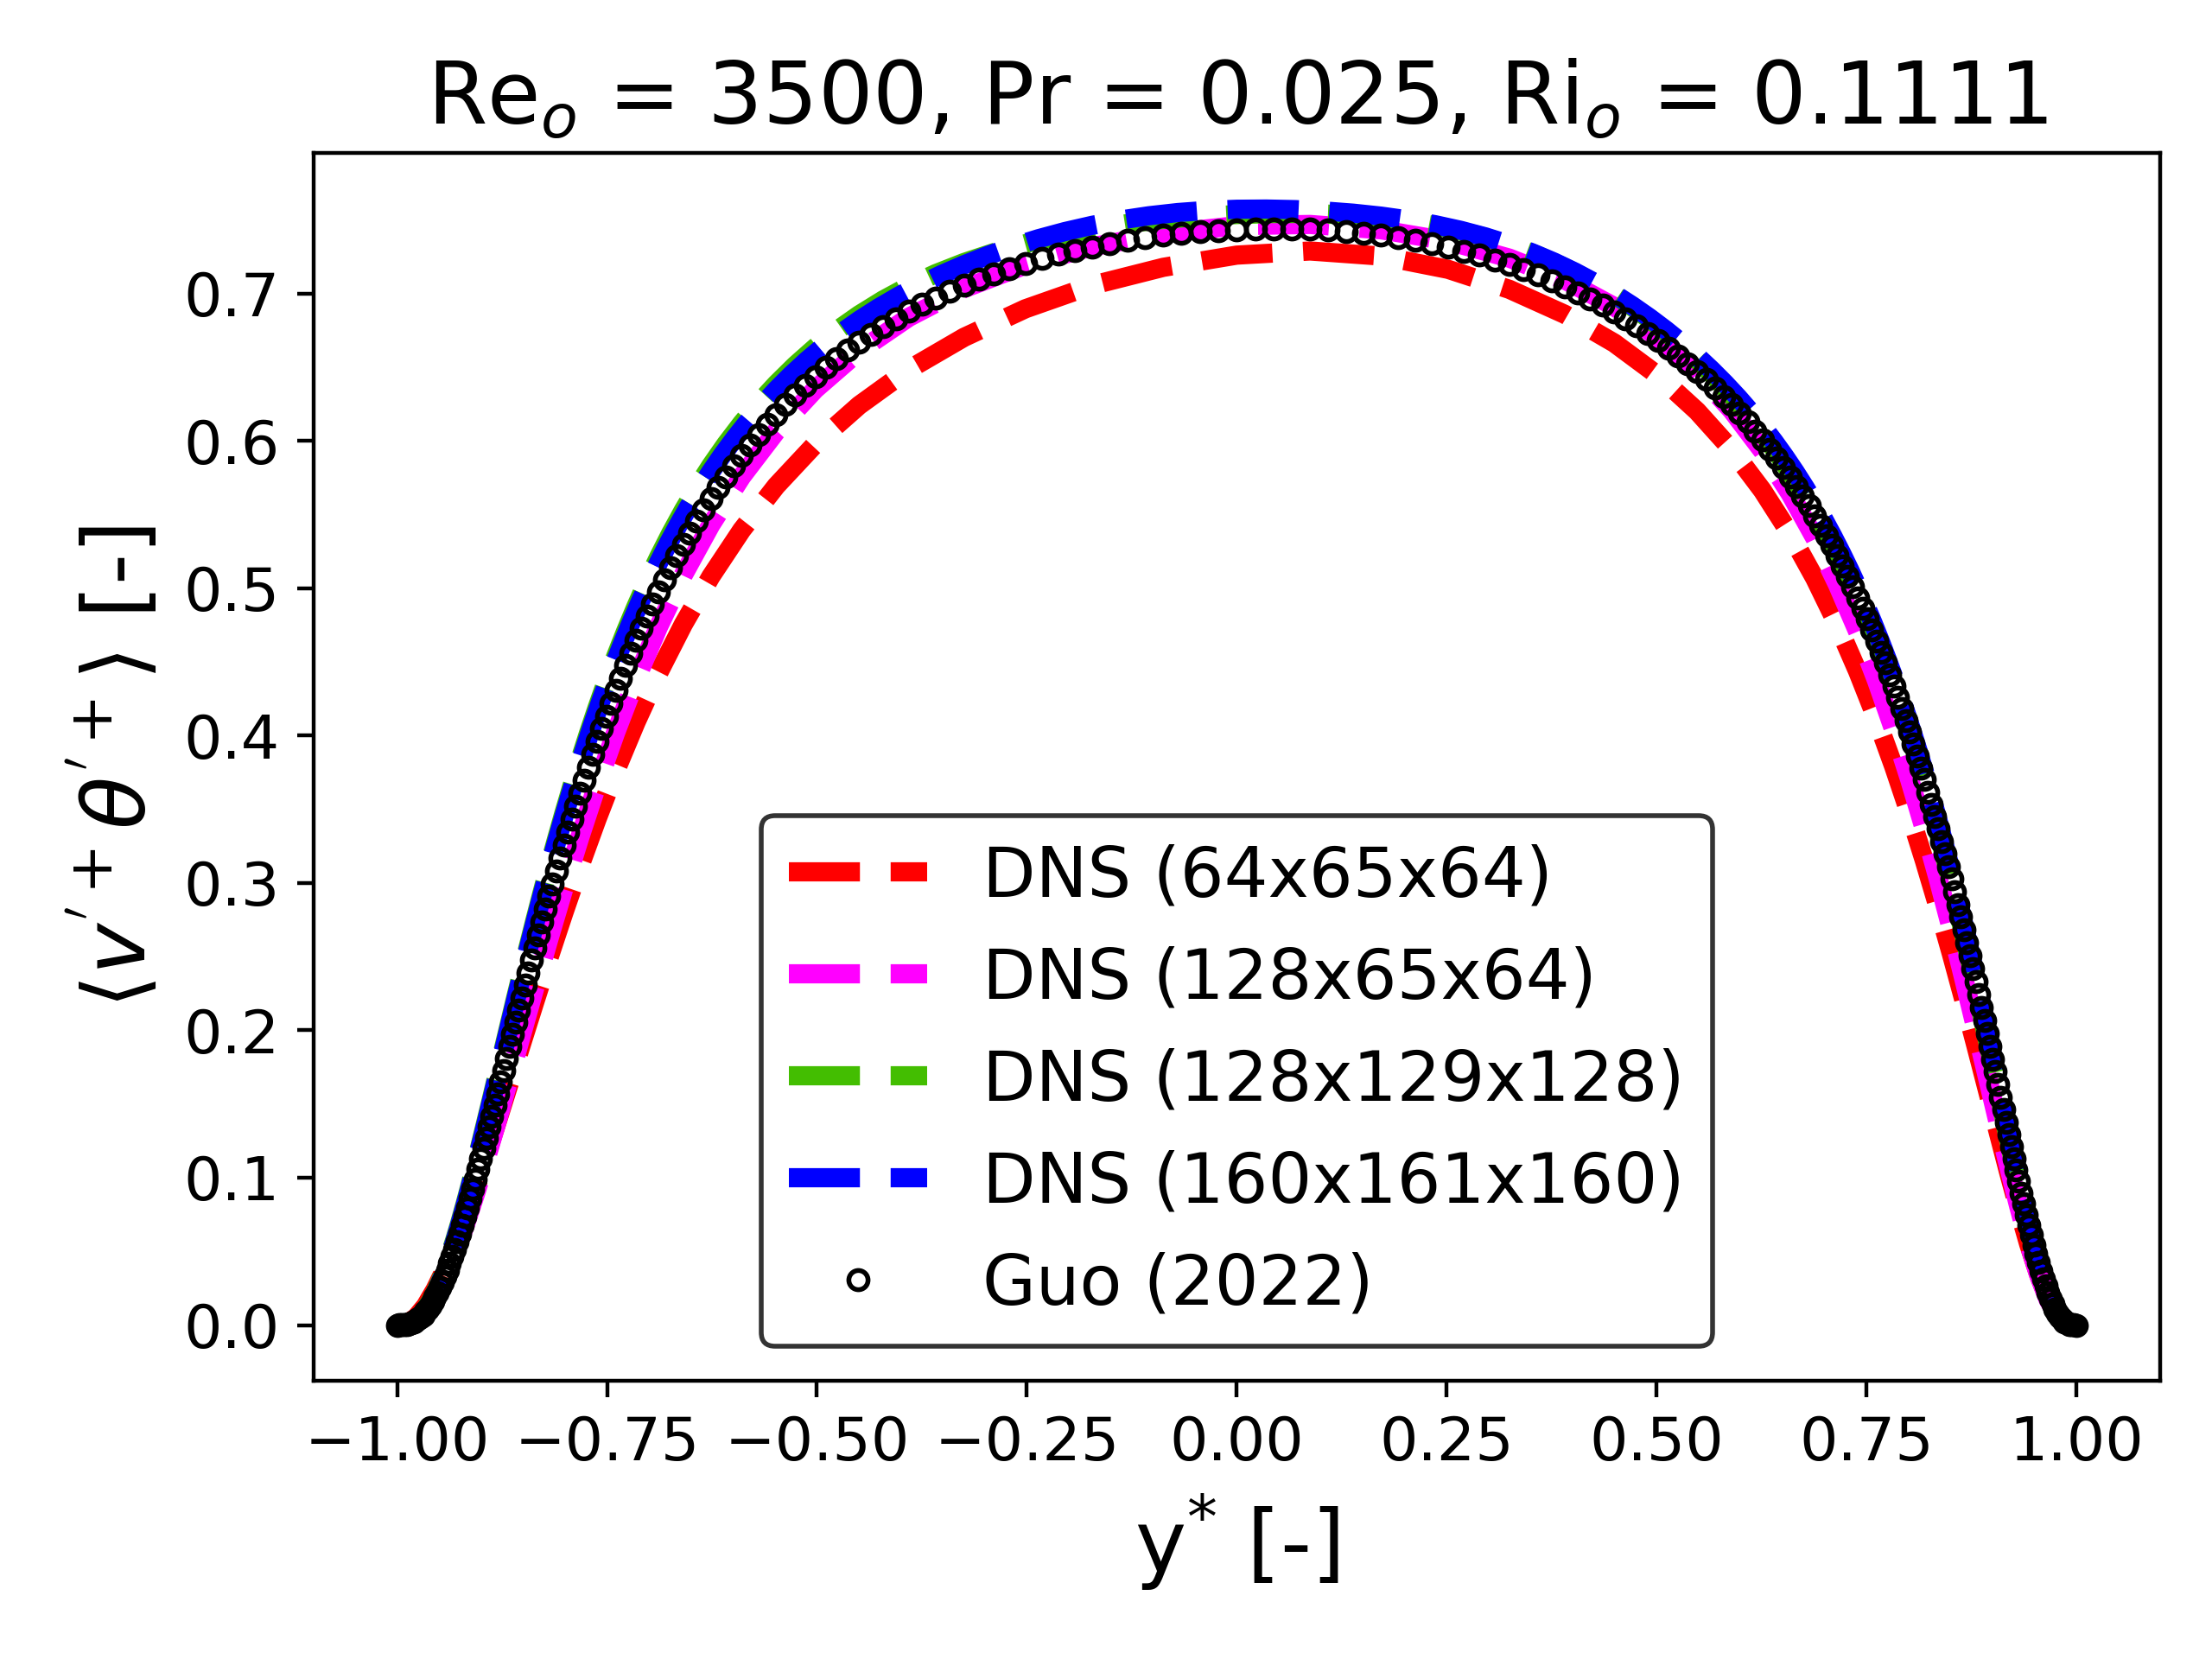
\includegraphics[width=0.49\textwidth]{results/guo/rib05/mct_vp_thetap.png}
    \label{fig:phi_vp_thetap_guo}}  
    
   \caption{a) Perfiles de temperatura media. b) Fluctuaciones de la temperatura. c) Perfiles de la velocidad media en la dirección de la corriente. d) Fluctuaciones de la velocidad en la dirección de la corriente. e) Flujo turbulento de calor en la dirección X. f) Flujo turbulento de calor en la dirección Y.} 
 
 \label{fig:guo}
\end{figure}


\subsubsection{Variación de dominio}

\begin{figure}[H]
 \centering

  \subfloat[]{
    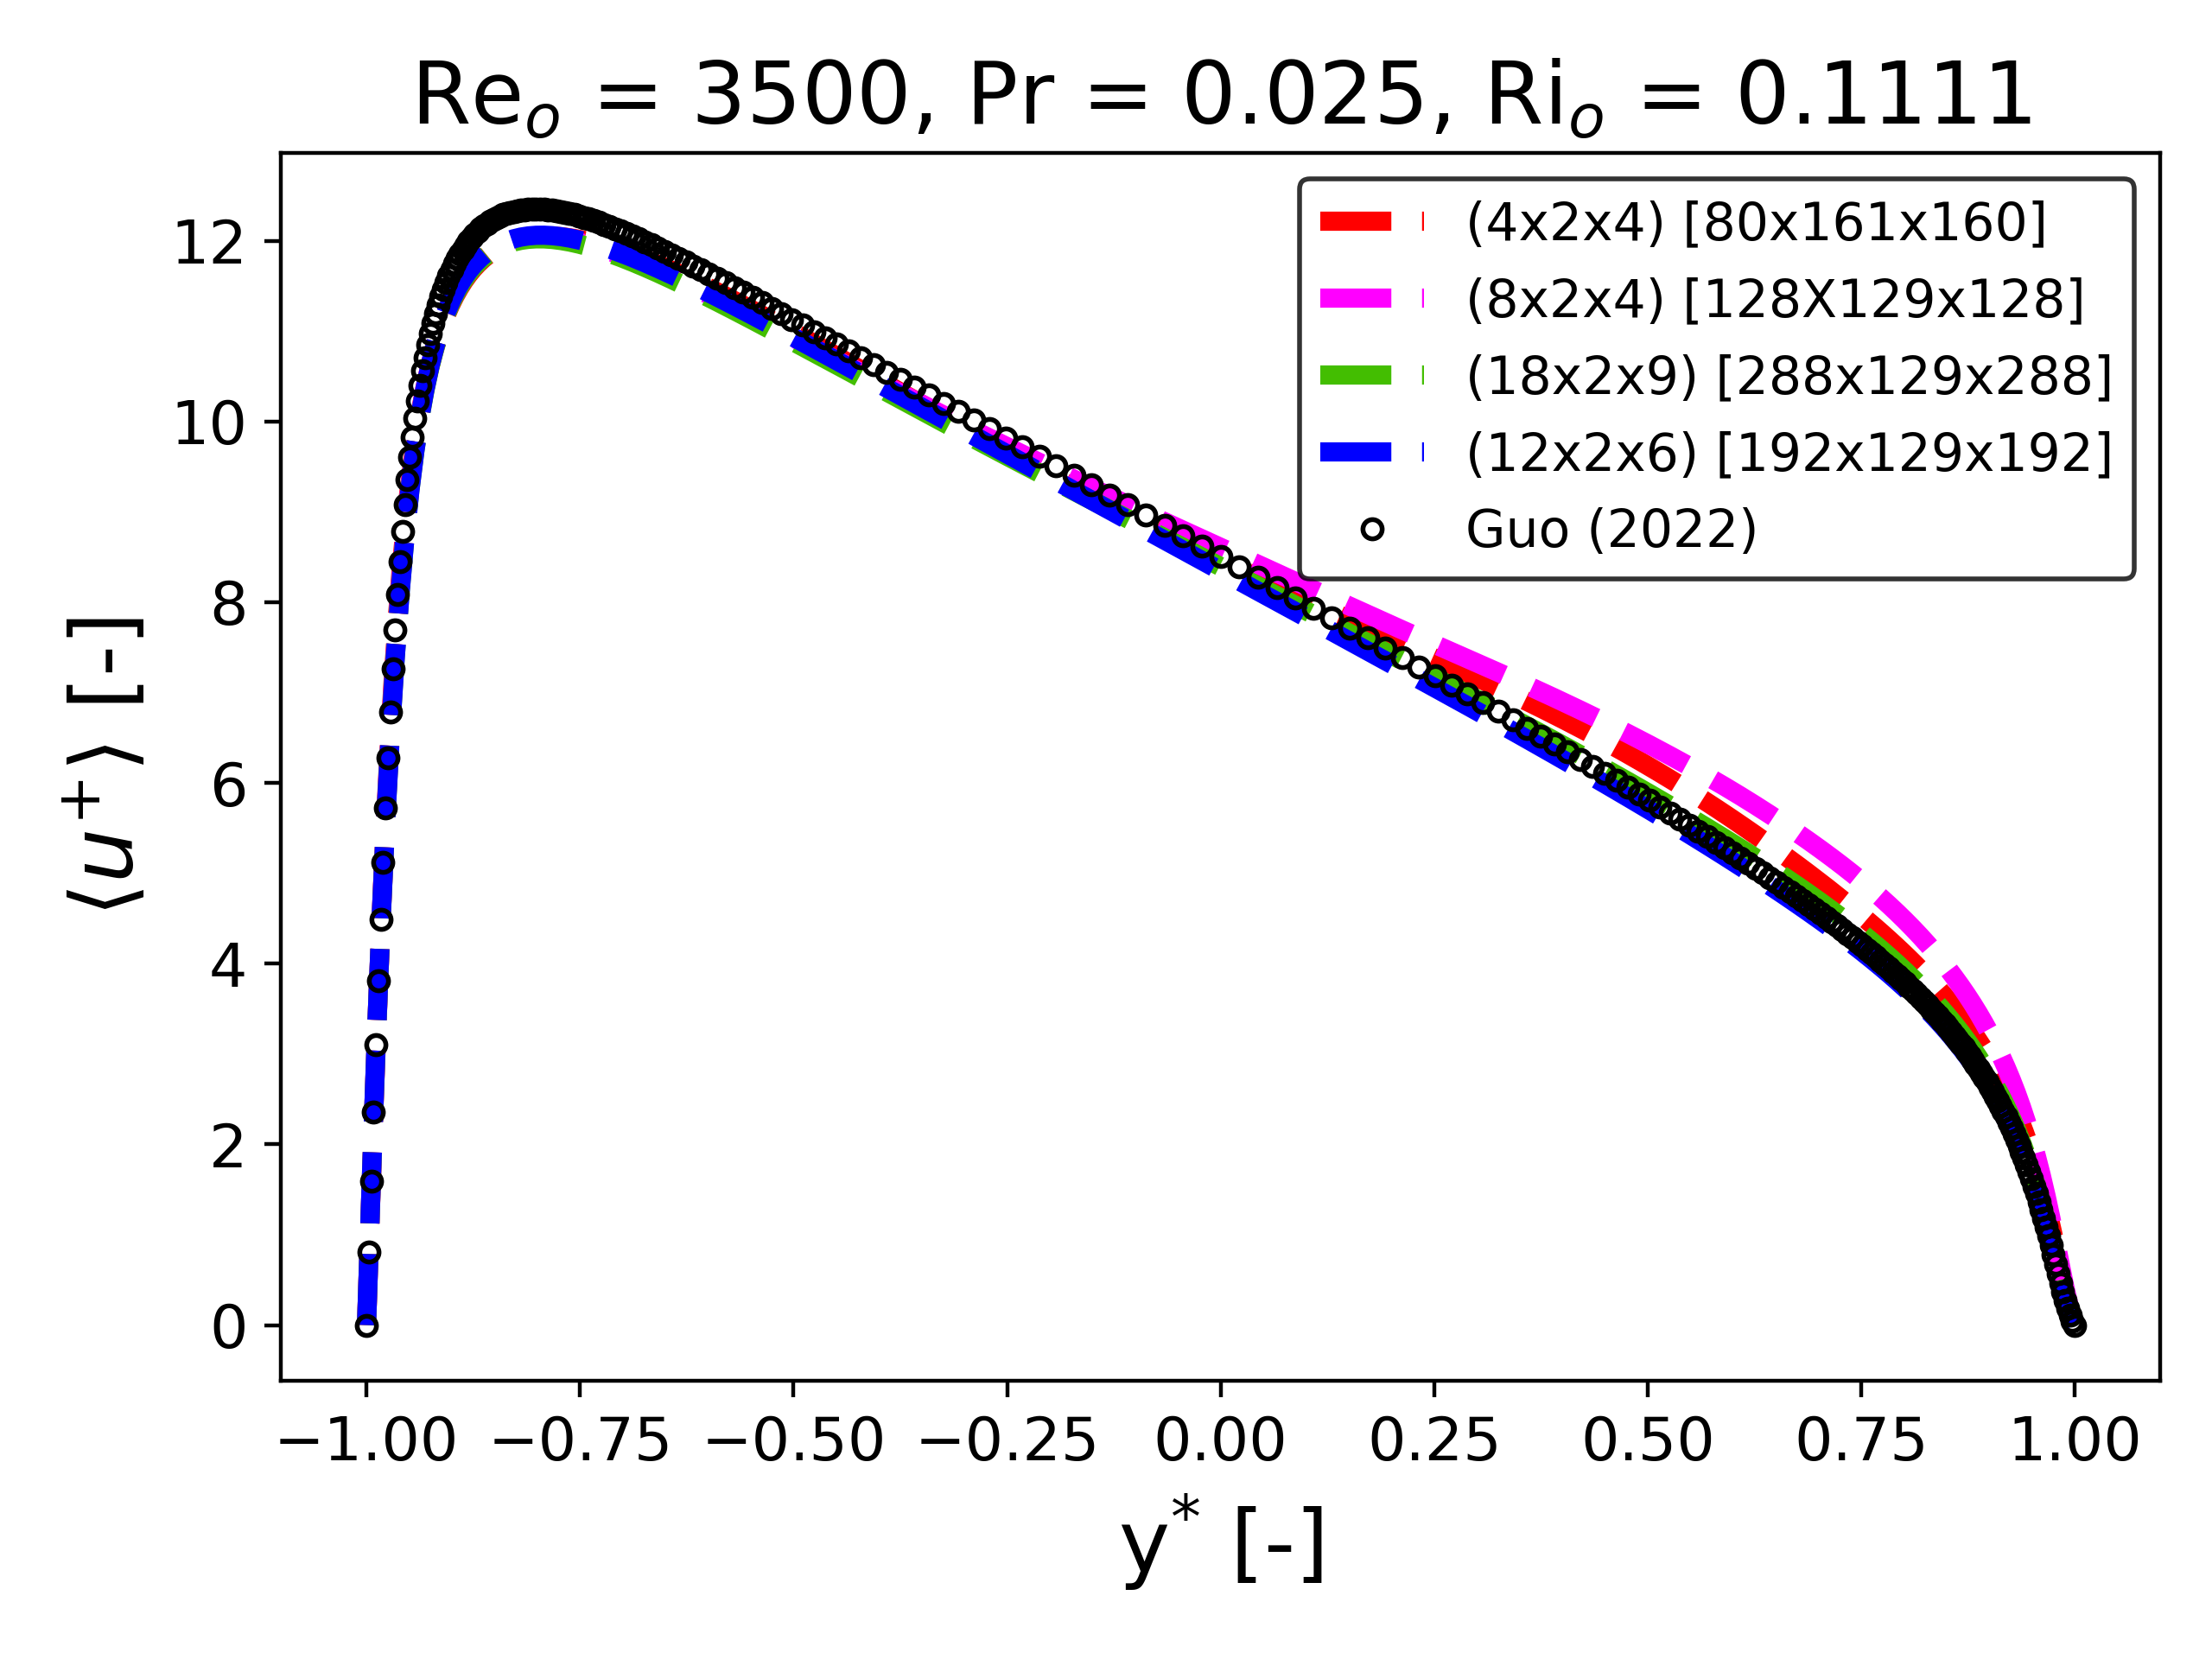
\includegraphics[width=0.49\textwidth]{results/guo/rib05_domains/mct_upmean.png}
    \label{fig:phi_mean_guo}}  
  \subfloat[]{
    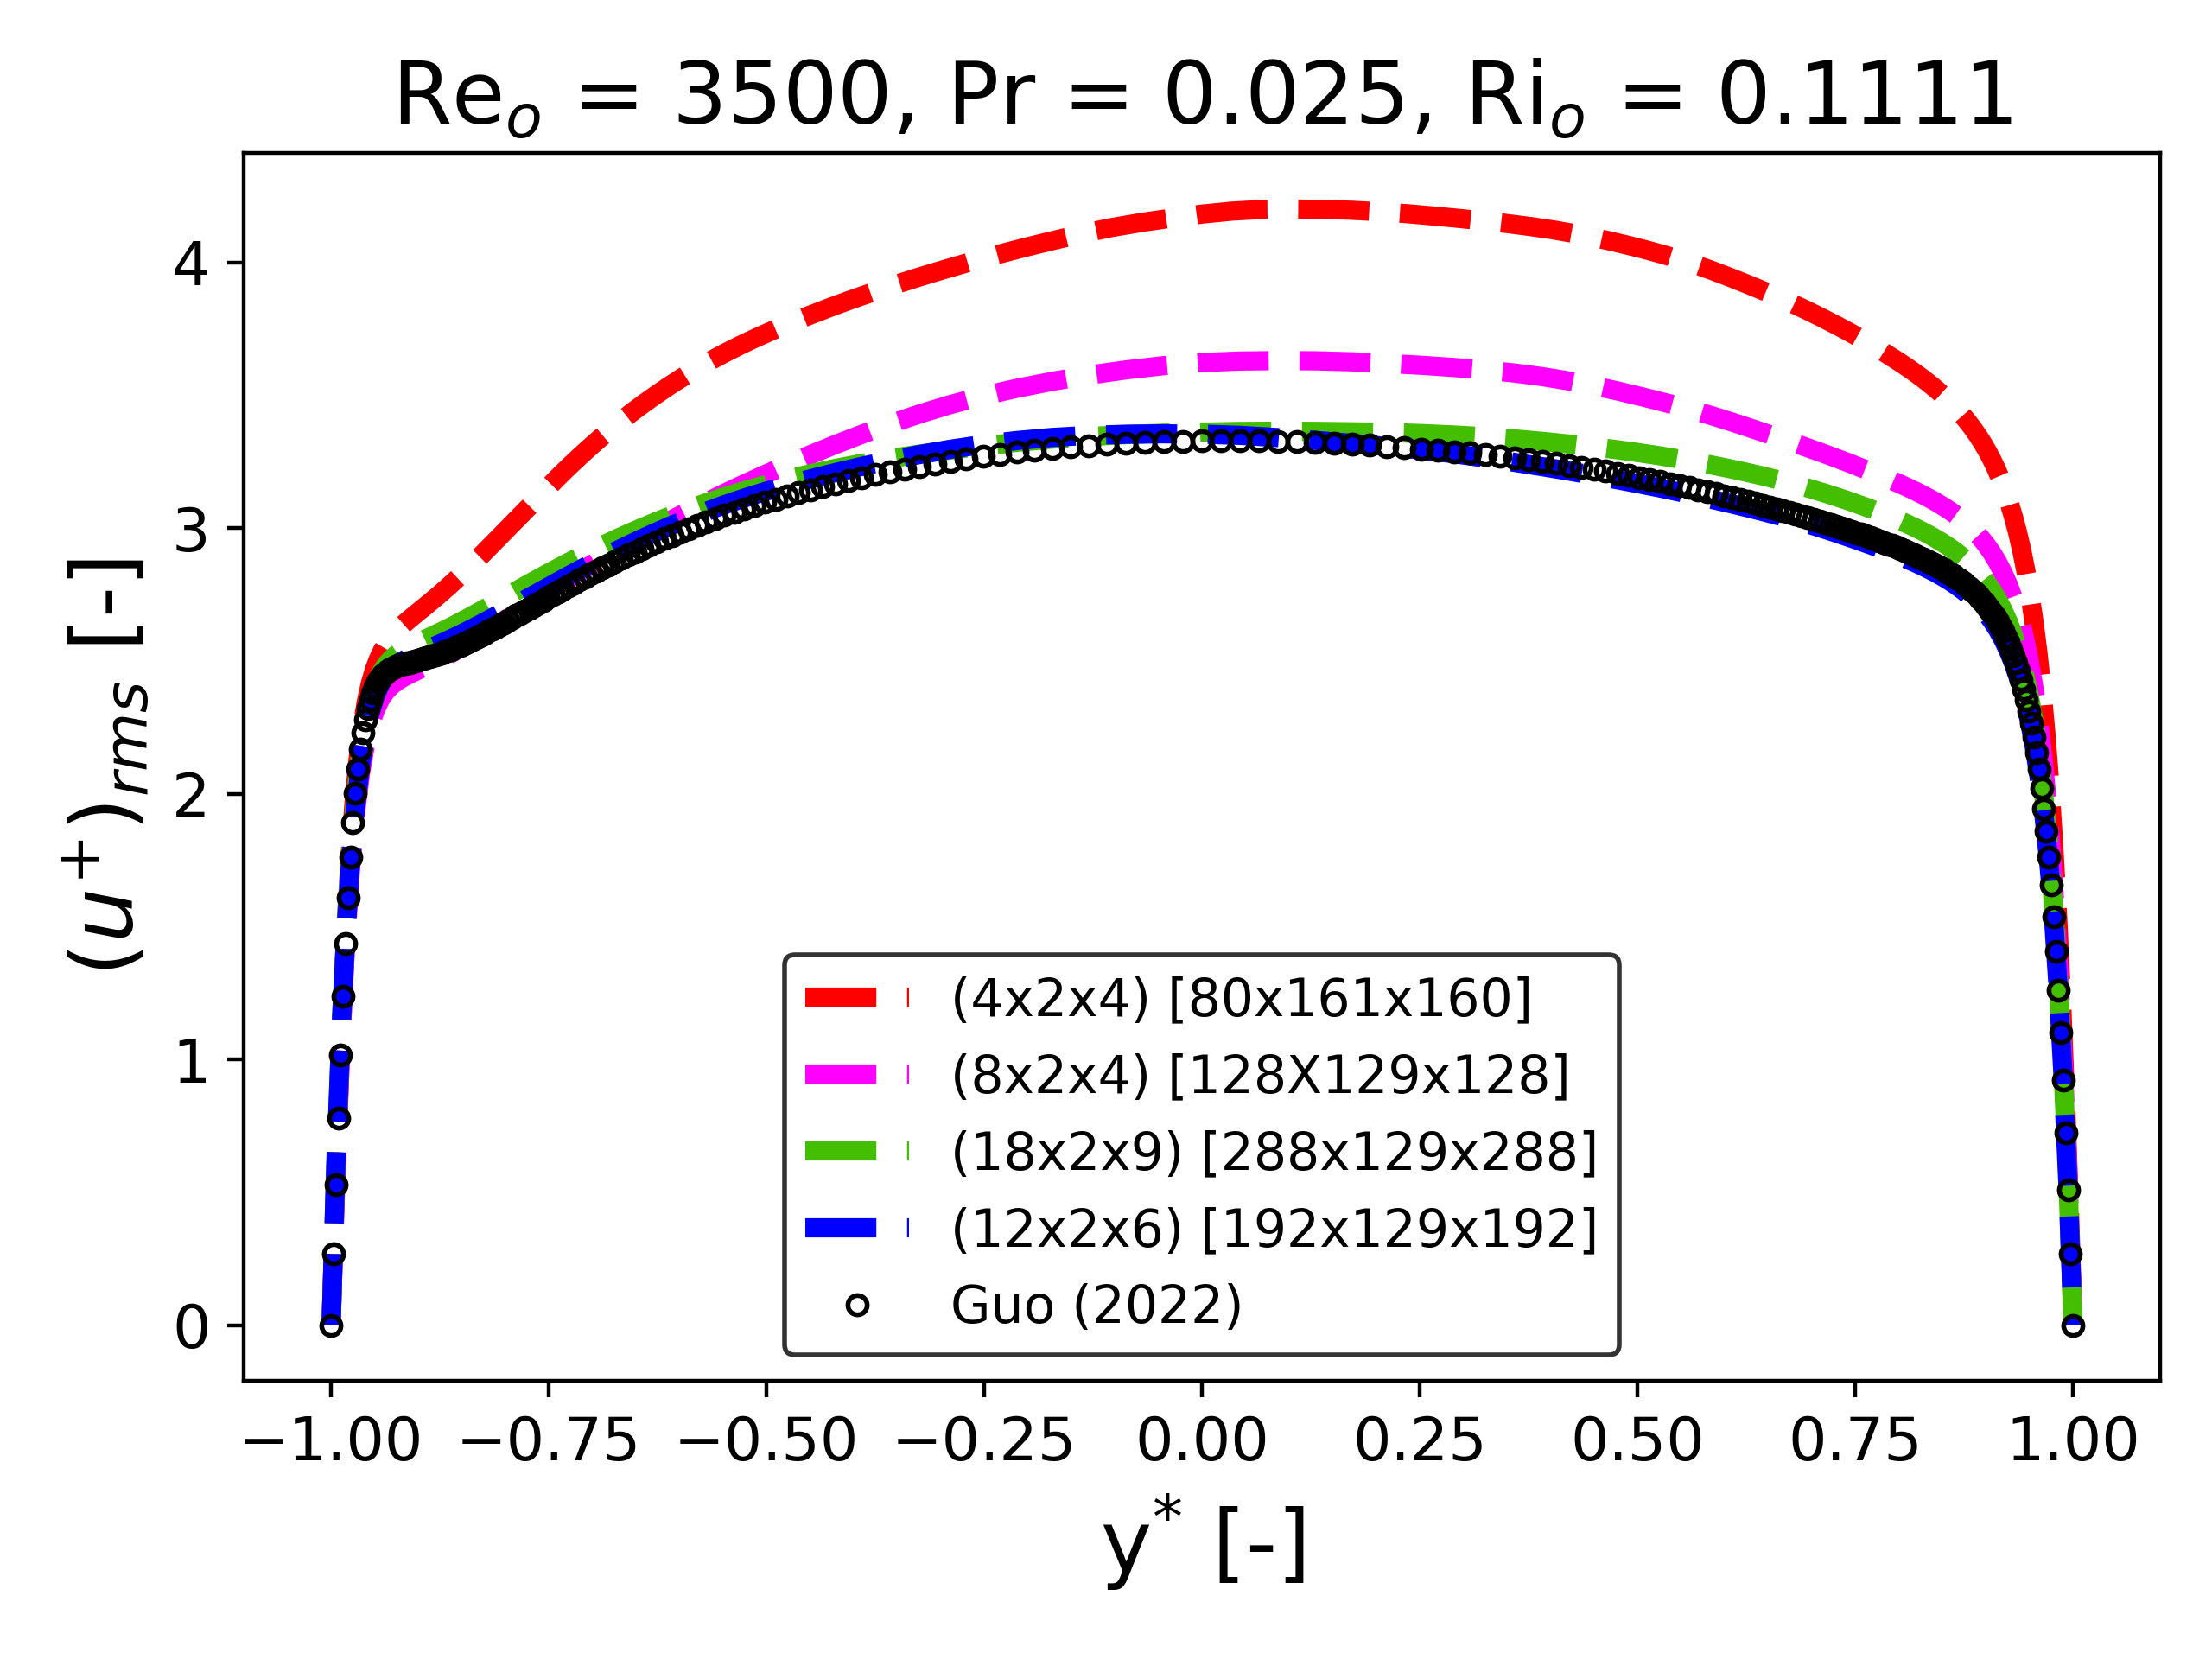
\includegraphics[width=0.49\textwidth]{results/guo/rib05_domains/mct_uprms.png}
    \label{fig:phi_rms_guo}} 
 
  \subfloat[]{
    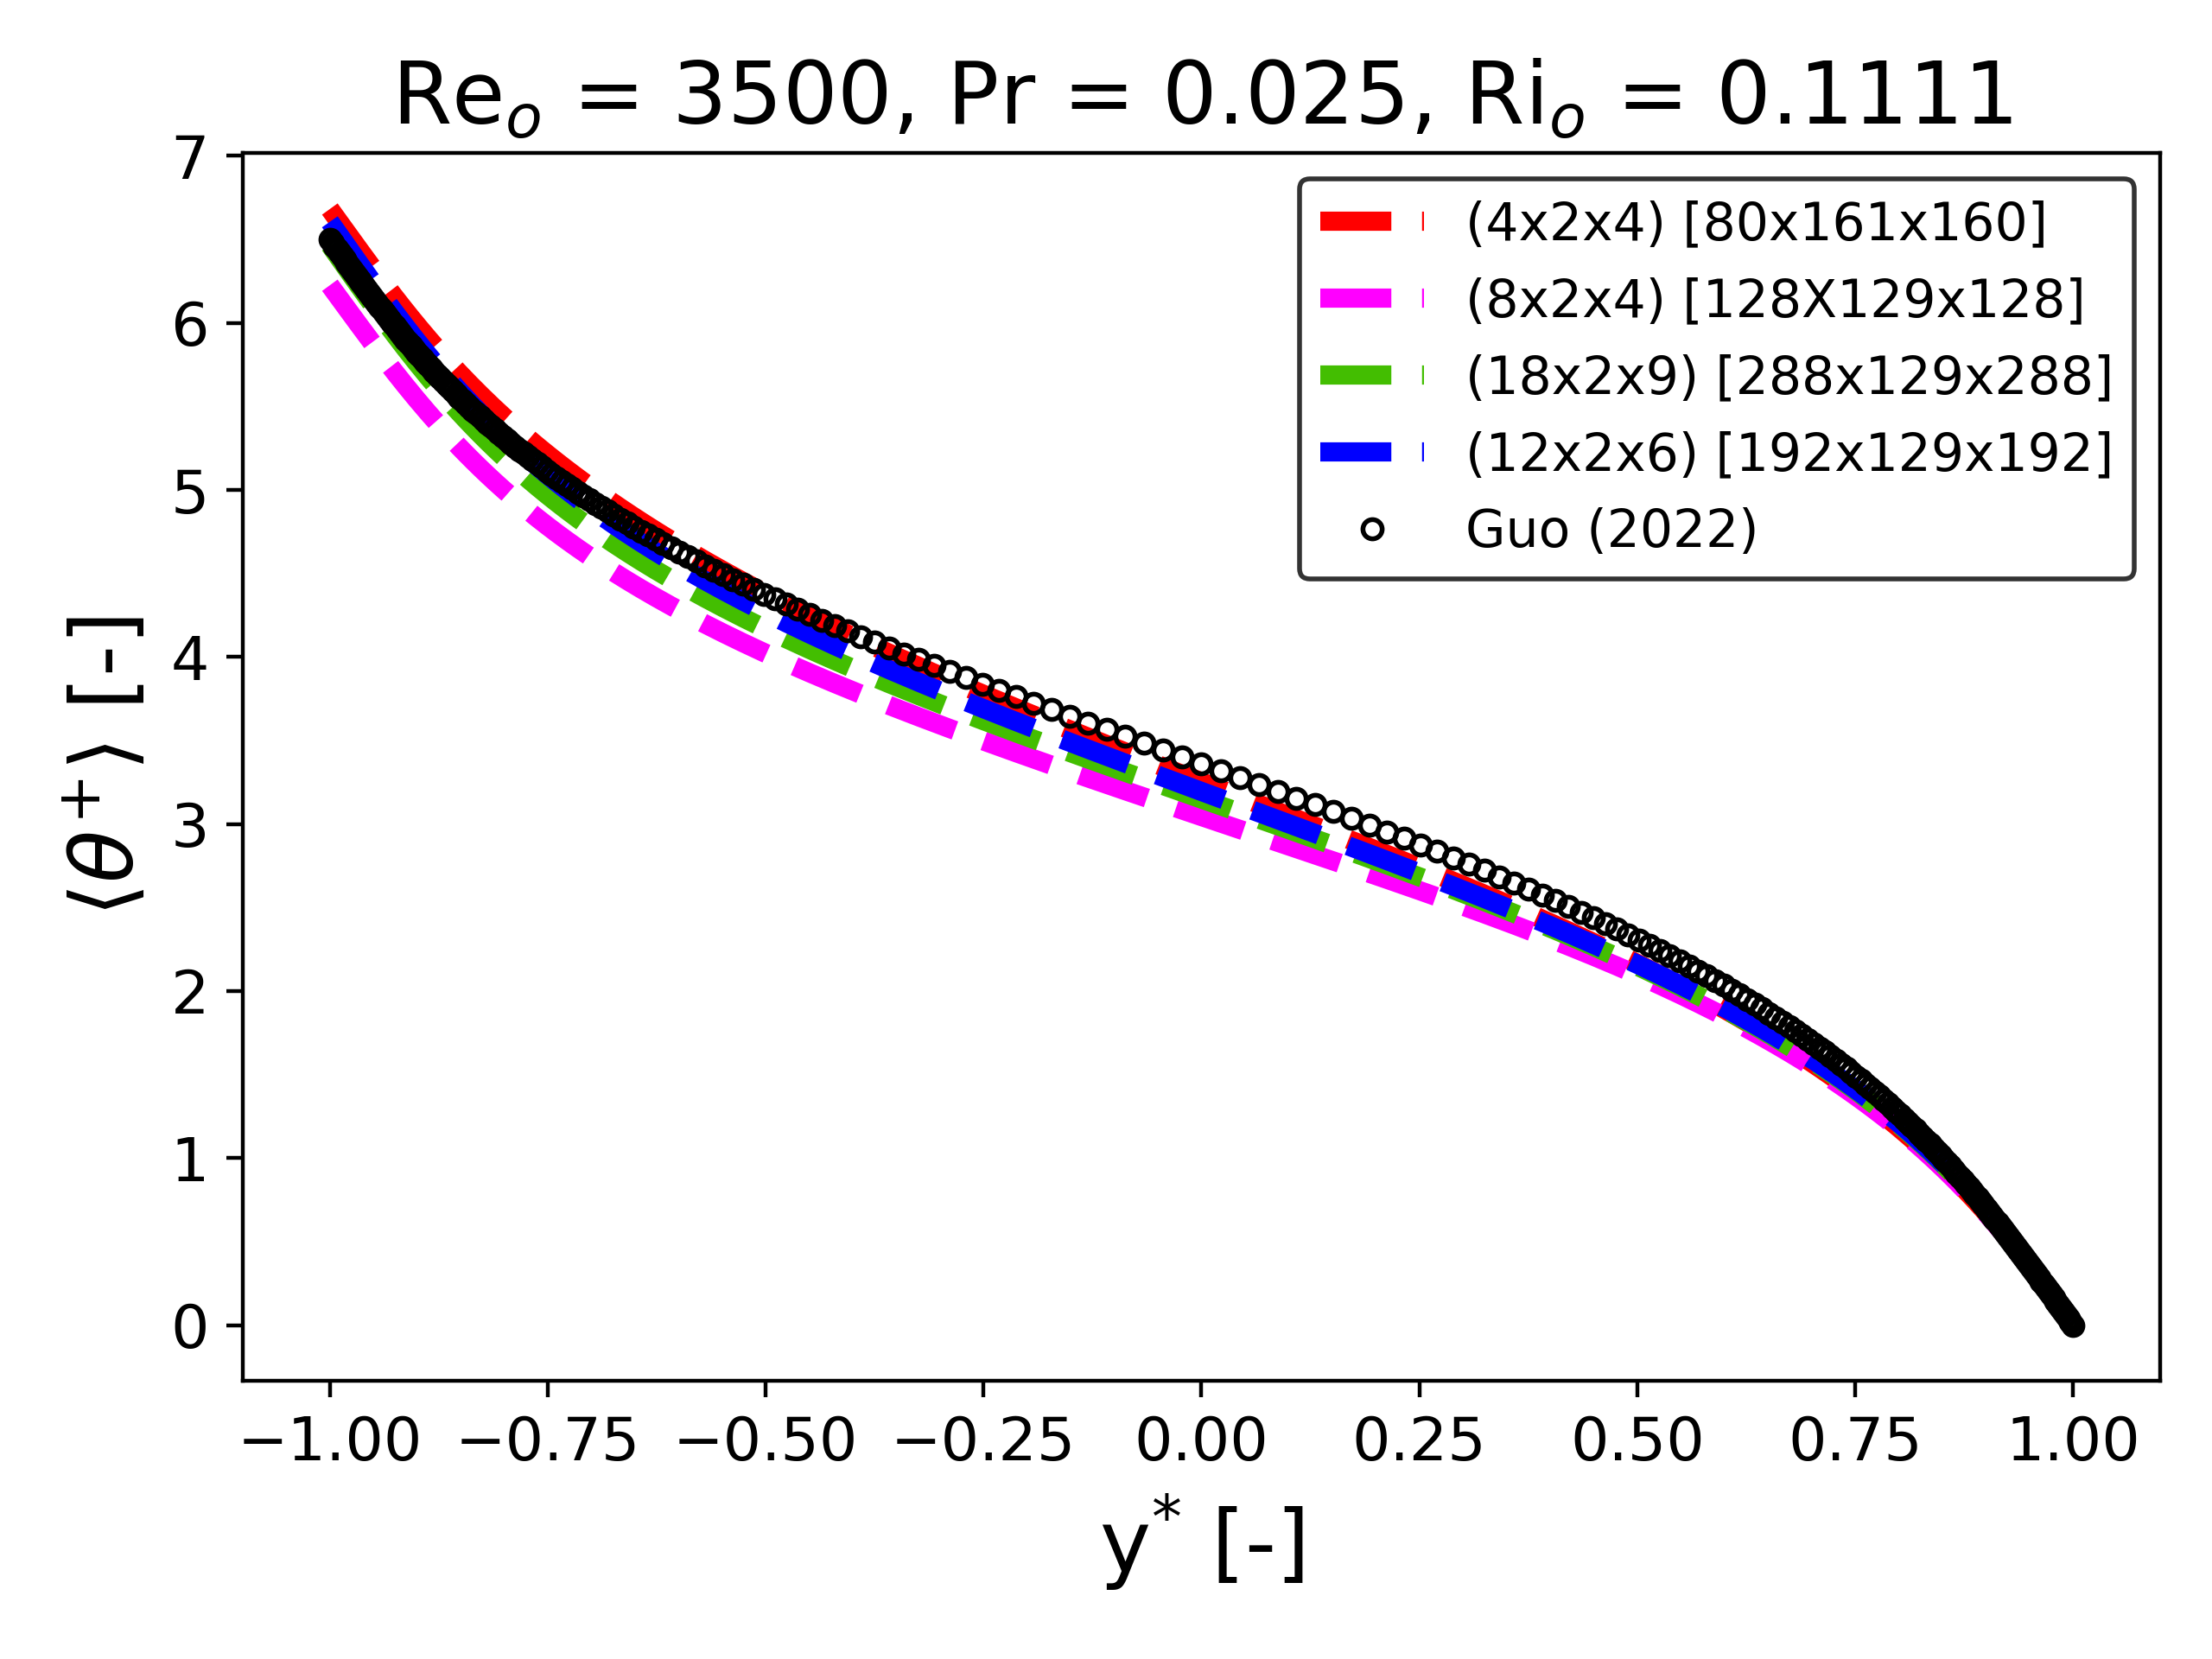
\includegraphics[width=0.49\textwidth]{results/guo/rib05_domains/mct_theta.png}
    \label{fig:phi_mean_guo}}  
  \subfloat[]{
    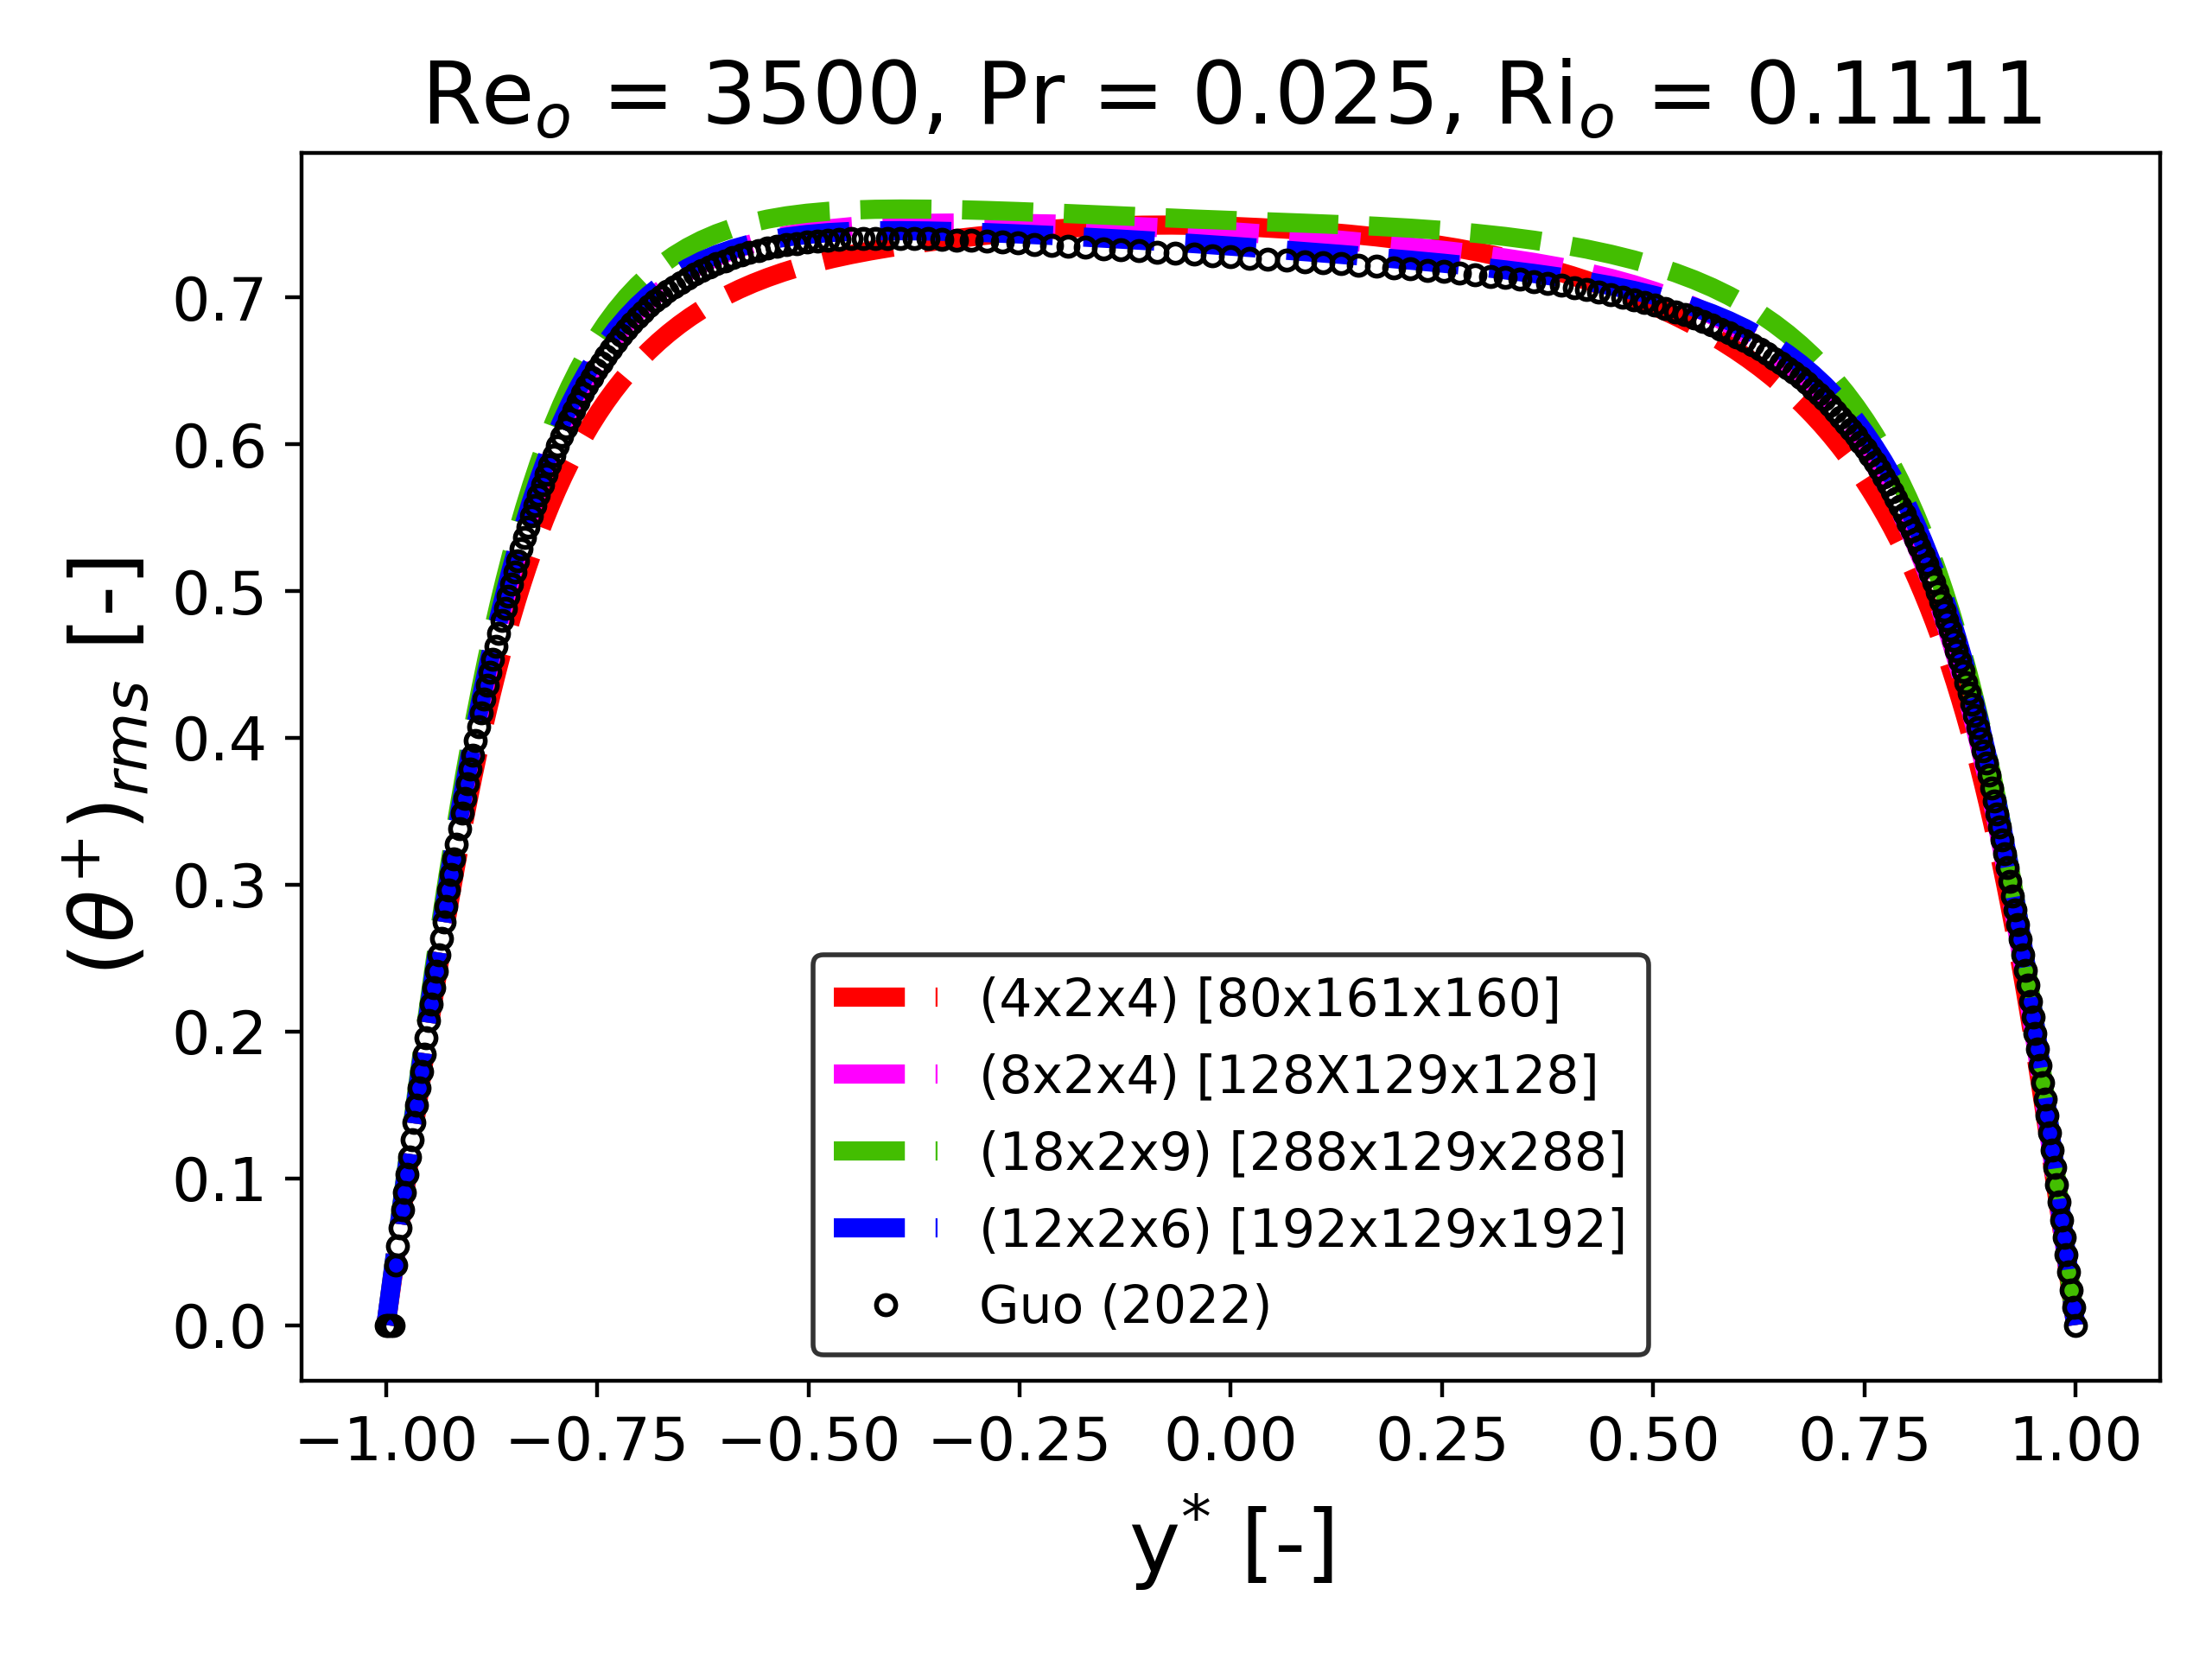
\includegraphics[width=0.49\textwidth]{results/guo/rib05_domains/mct_thetap_rms.png}
    \label{fig:phi_rms_guo}}  

  \subfloat[]{
    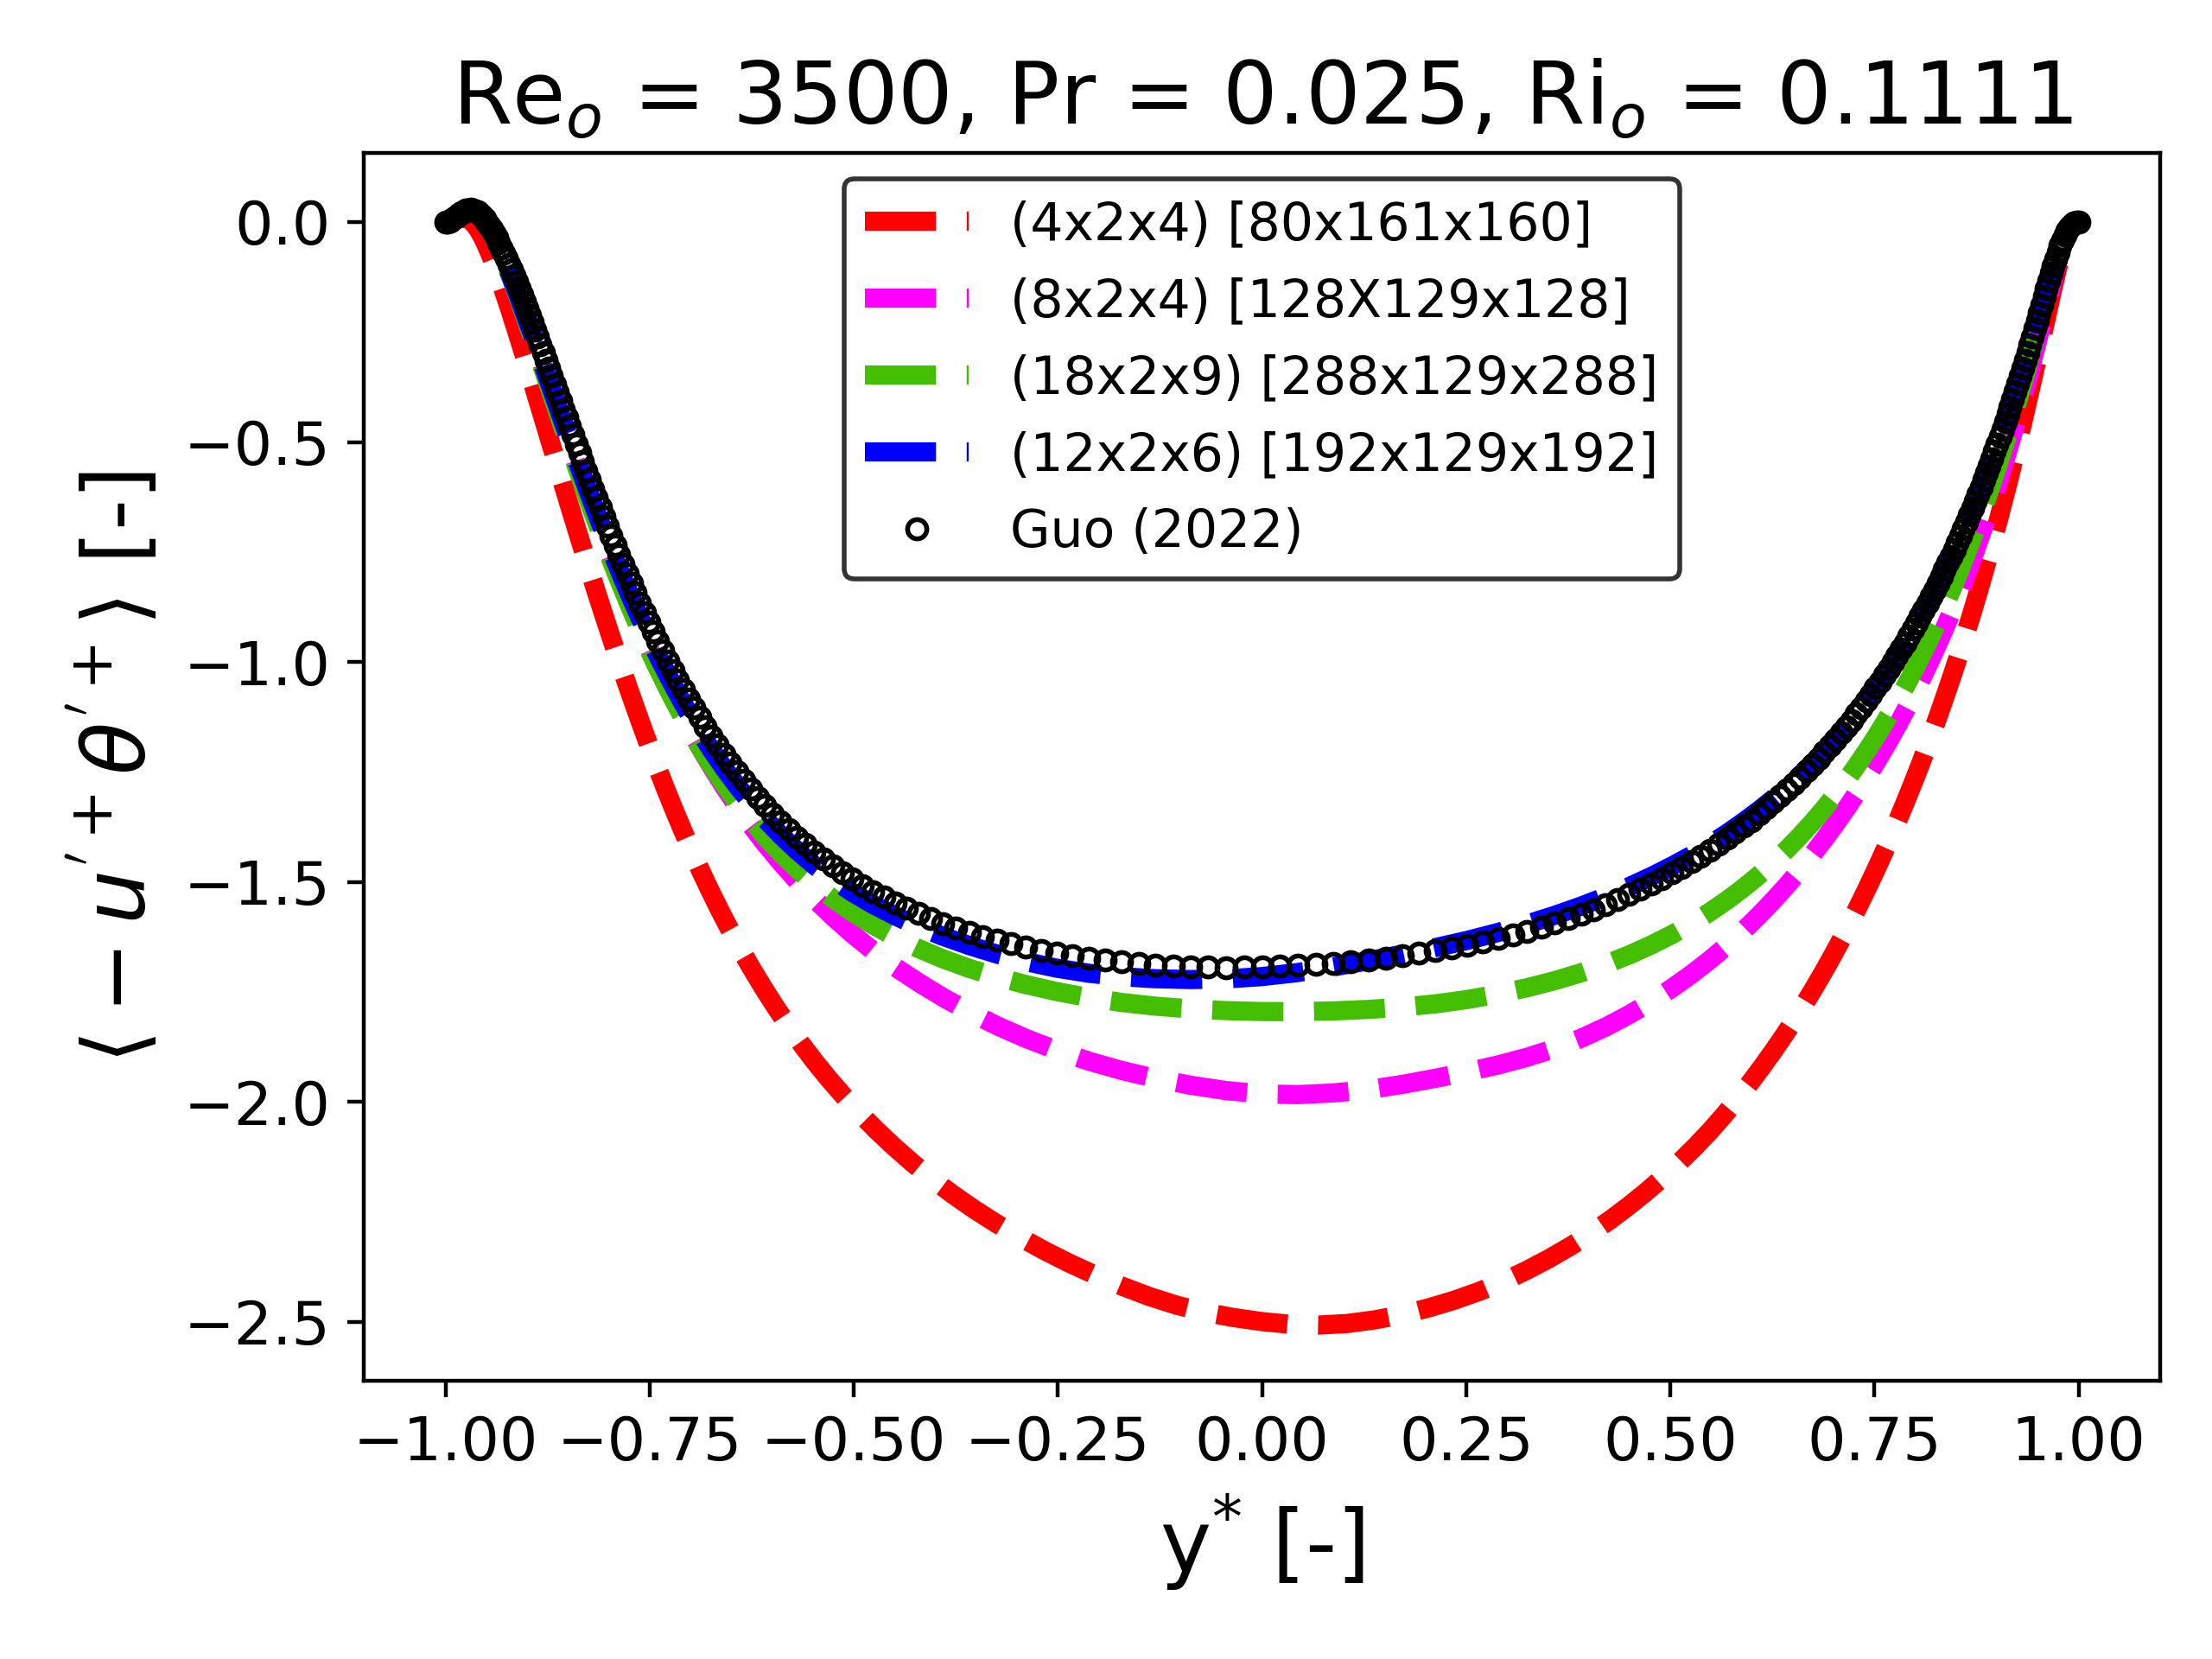
\includegraphics[width=0.49\textwidth]{results/guo/rib05_domains/mct_up_thetap.png}
    \label{fig:phi_up_thetap_guo}}
  \subfloat[]{
    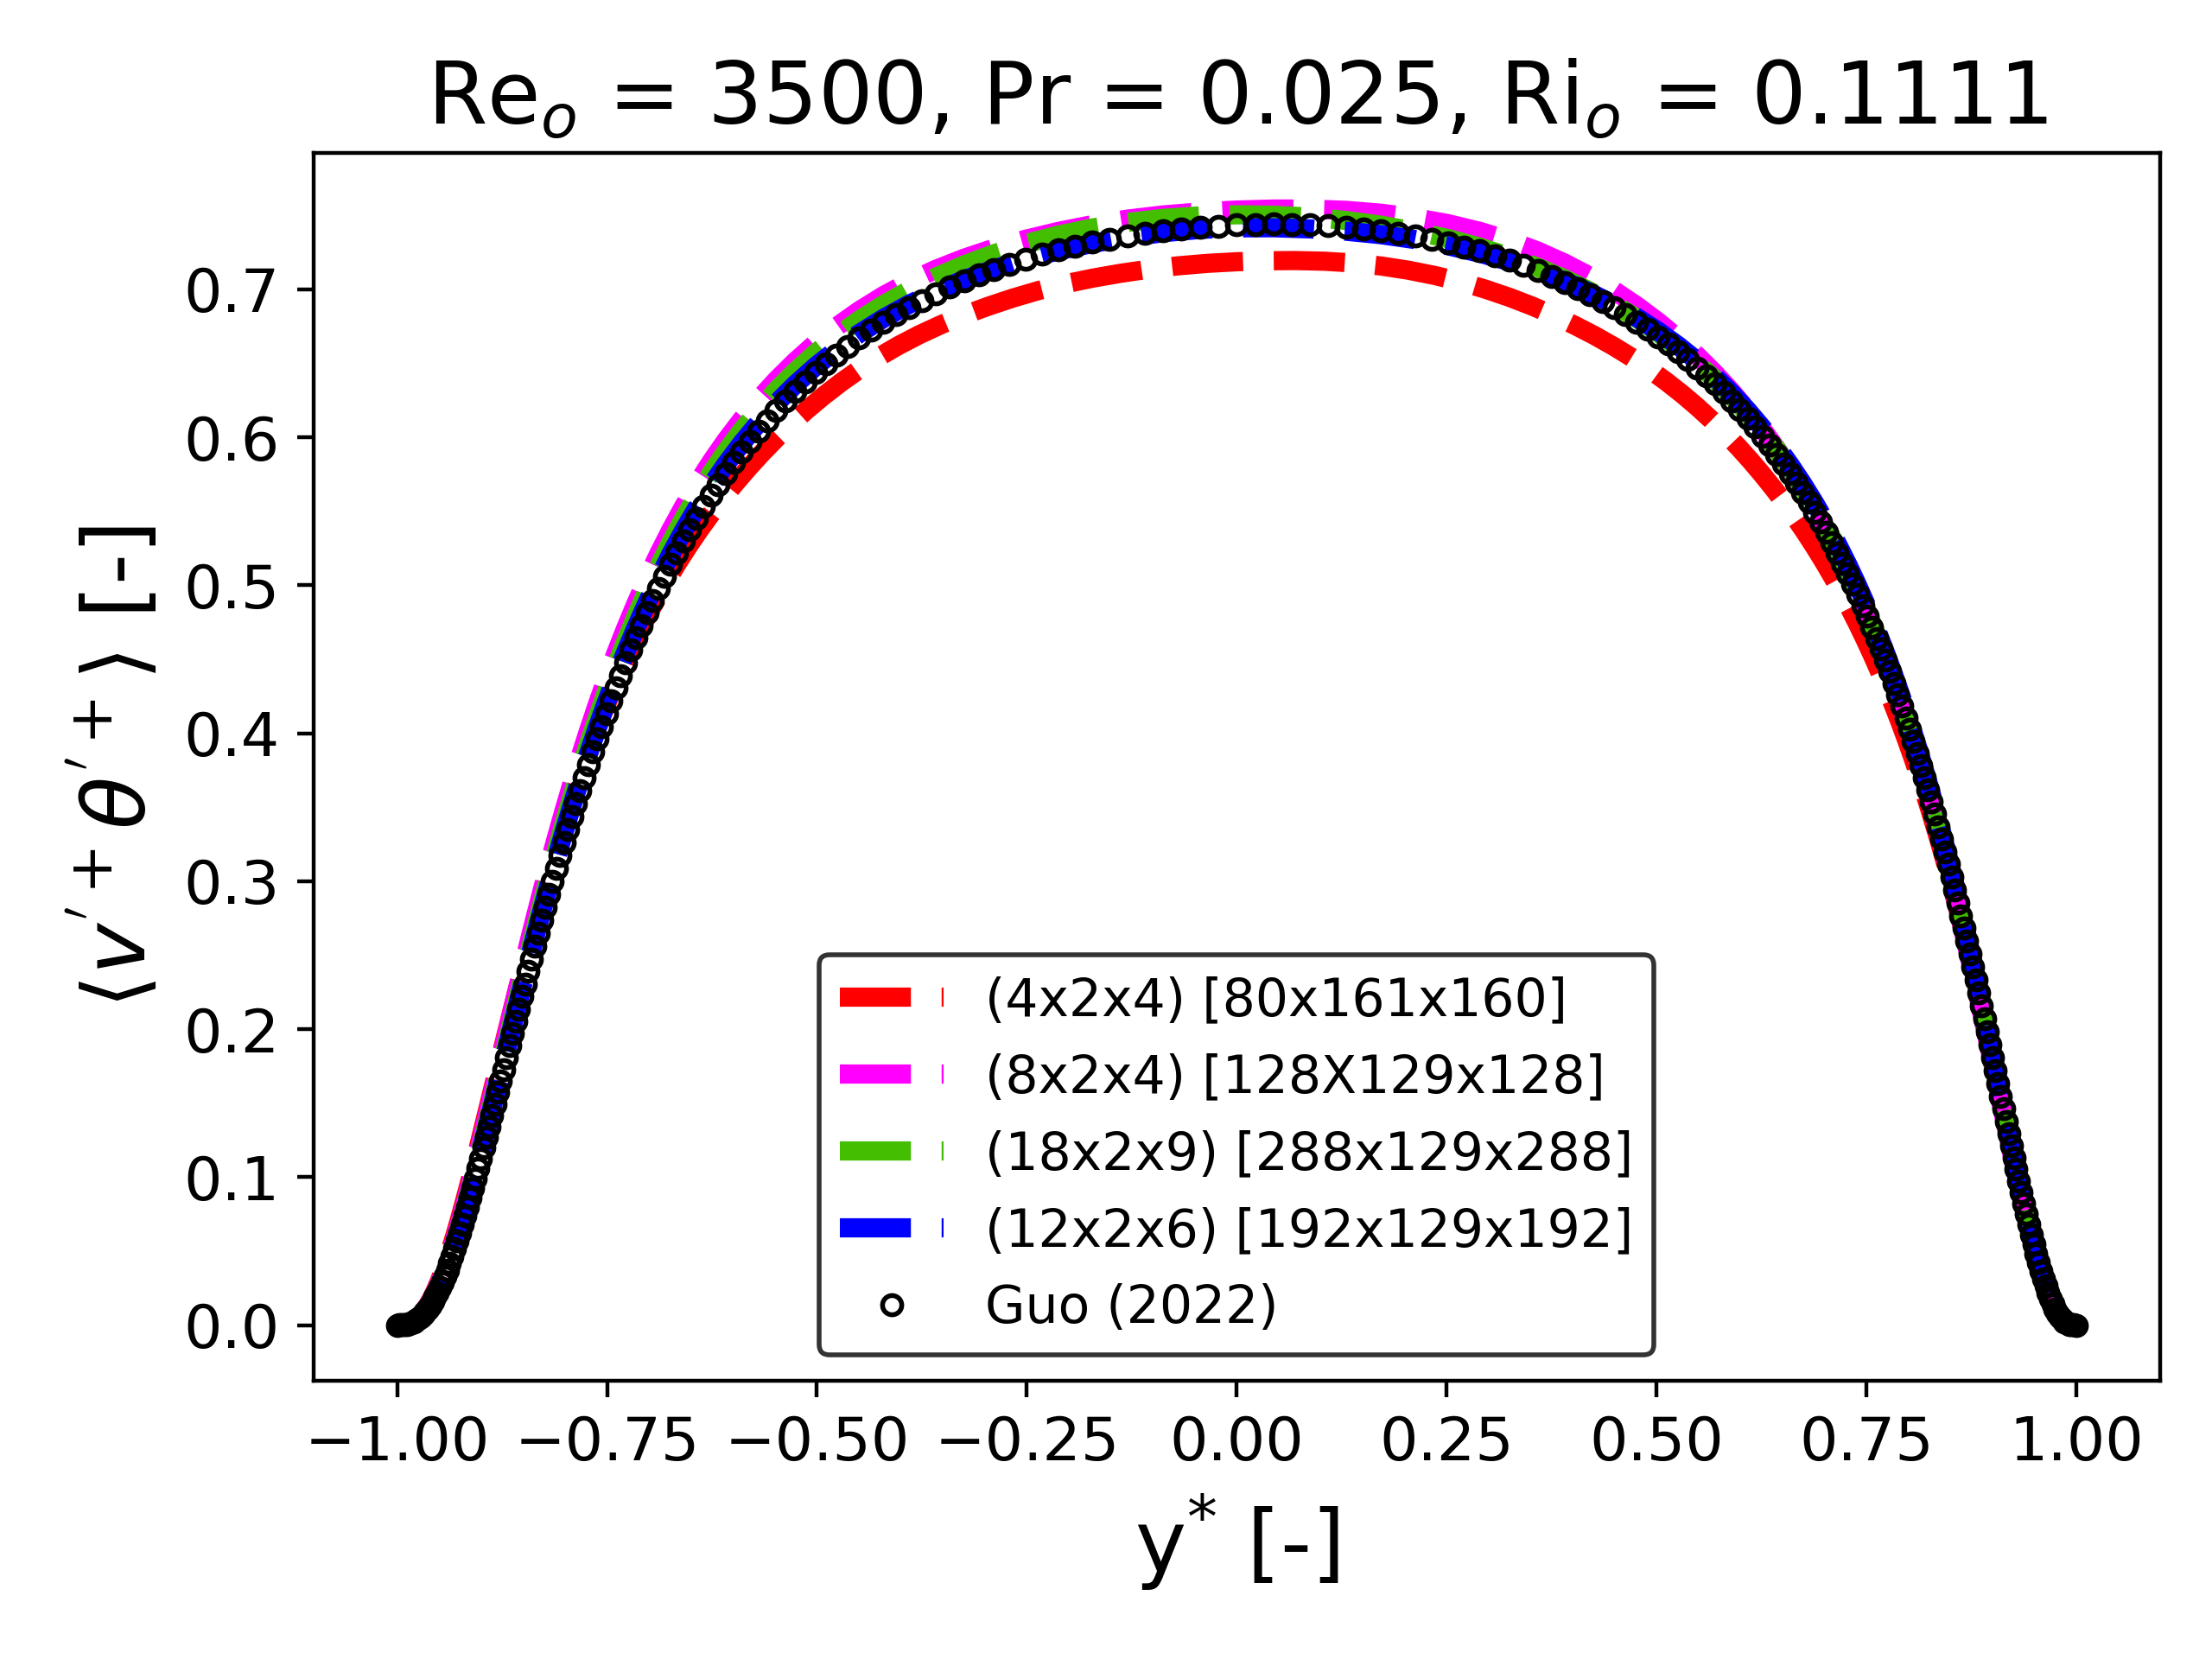
\includegraphics[width=0.49\textwidth]{results/guo/rib05_domains/mct_vp_thetap.png}
    \label{fig:phi_vp_thetap_guo}}  
    
   \caption{a) Perfiles de temperatura media. b) Fluctuaciones de la temperatura. c) Perfiles de la velocidad media en la dirección de la corriente. d) Fluctuaciones de la velocidad en la dirección de la corriente. e) Flujo turbulento de calor en la dirección X. f) Flujo turbulento de calor en la dirección Y.} 
 
 \label{fig:guo}
\end{figure}

\subsection{Caso $\mathbf{Ri_b}=0.25$}

\begin{figure}[H]
 \centering

  \subfloat[]{
    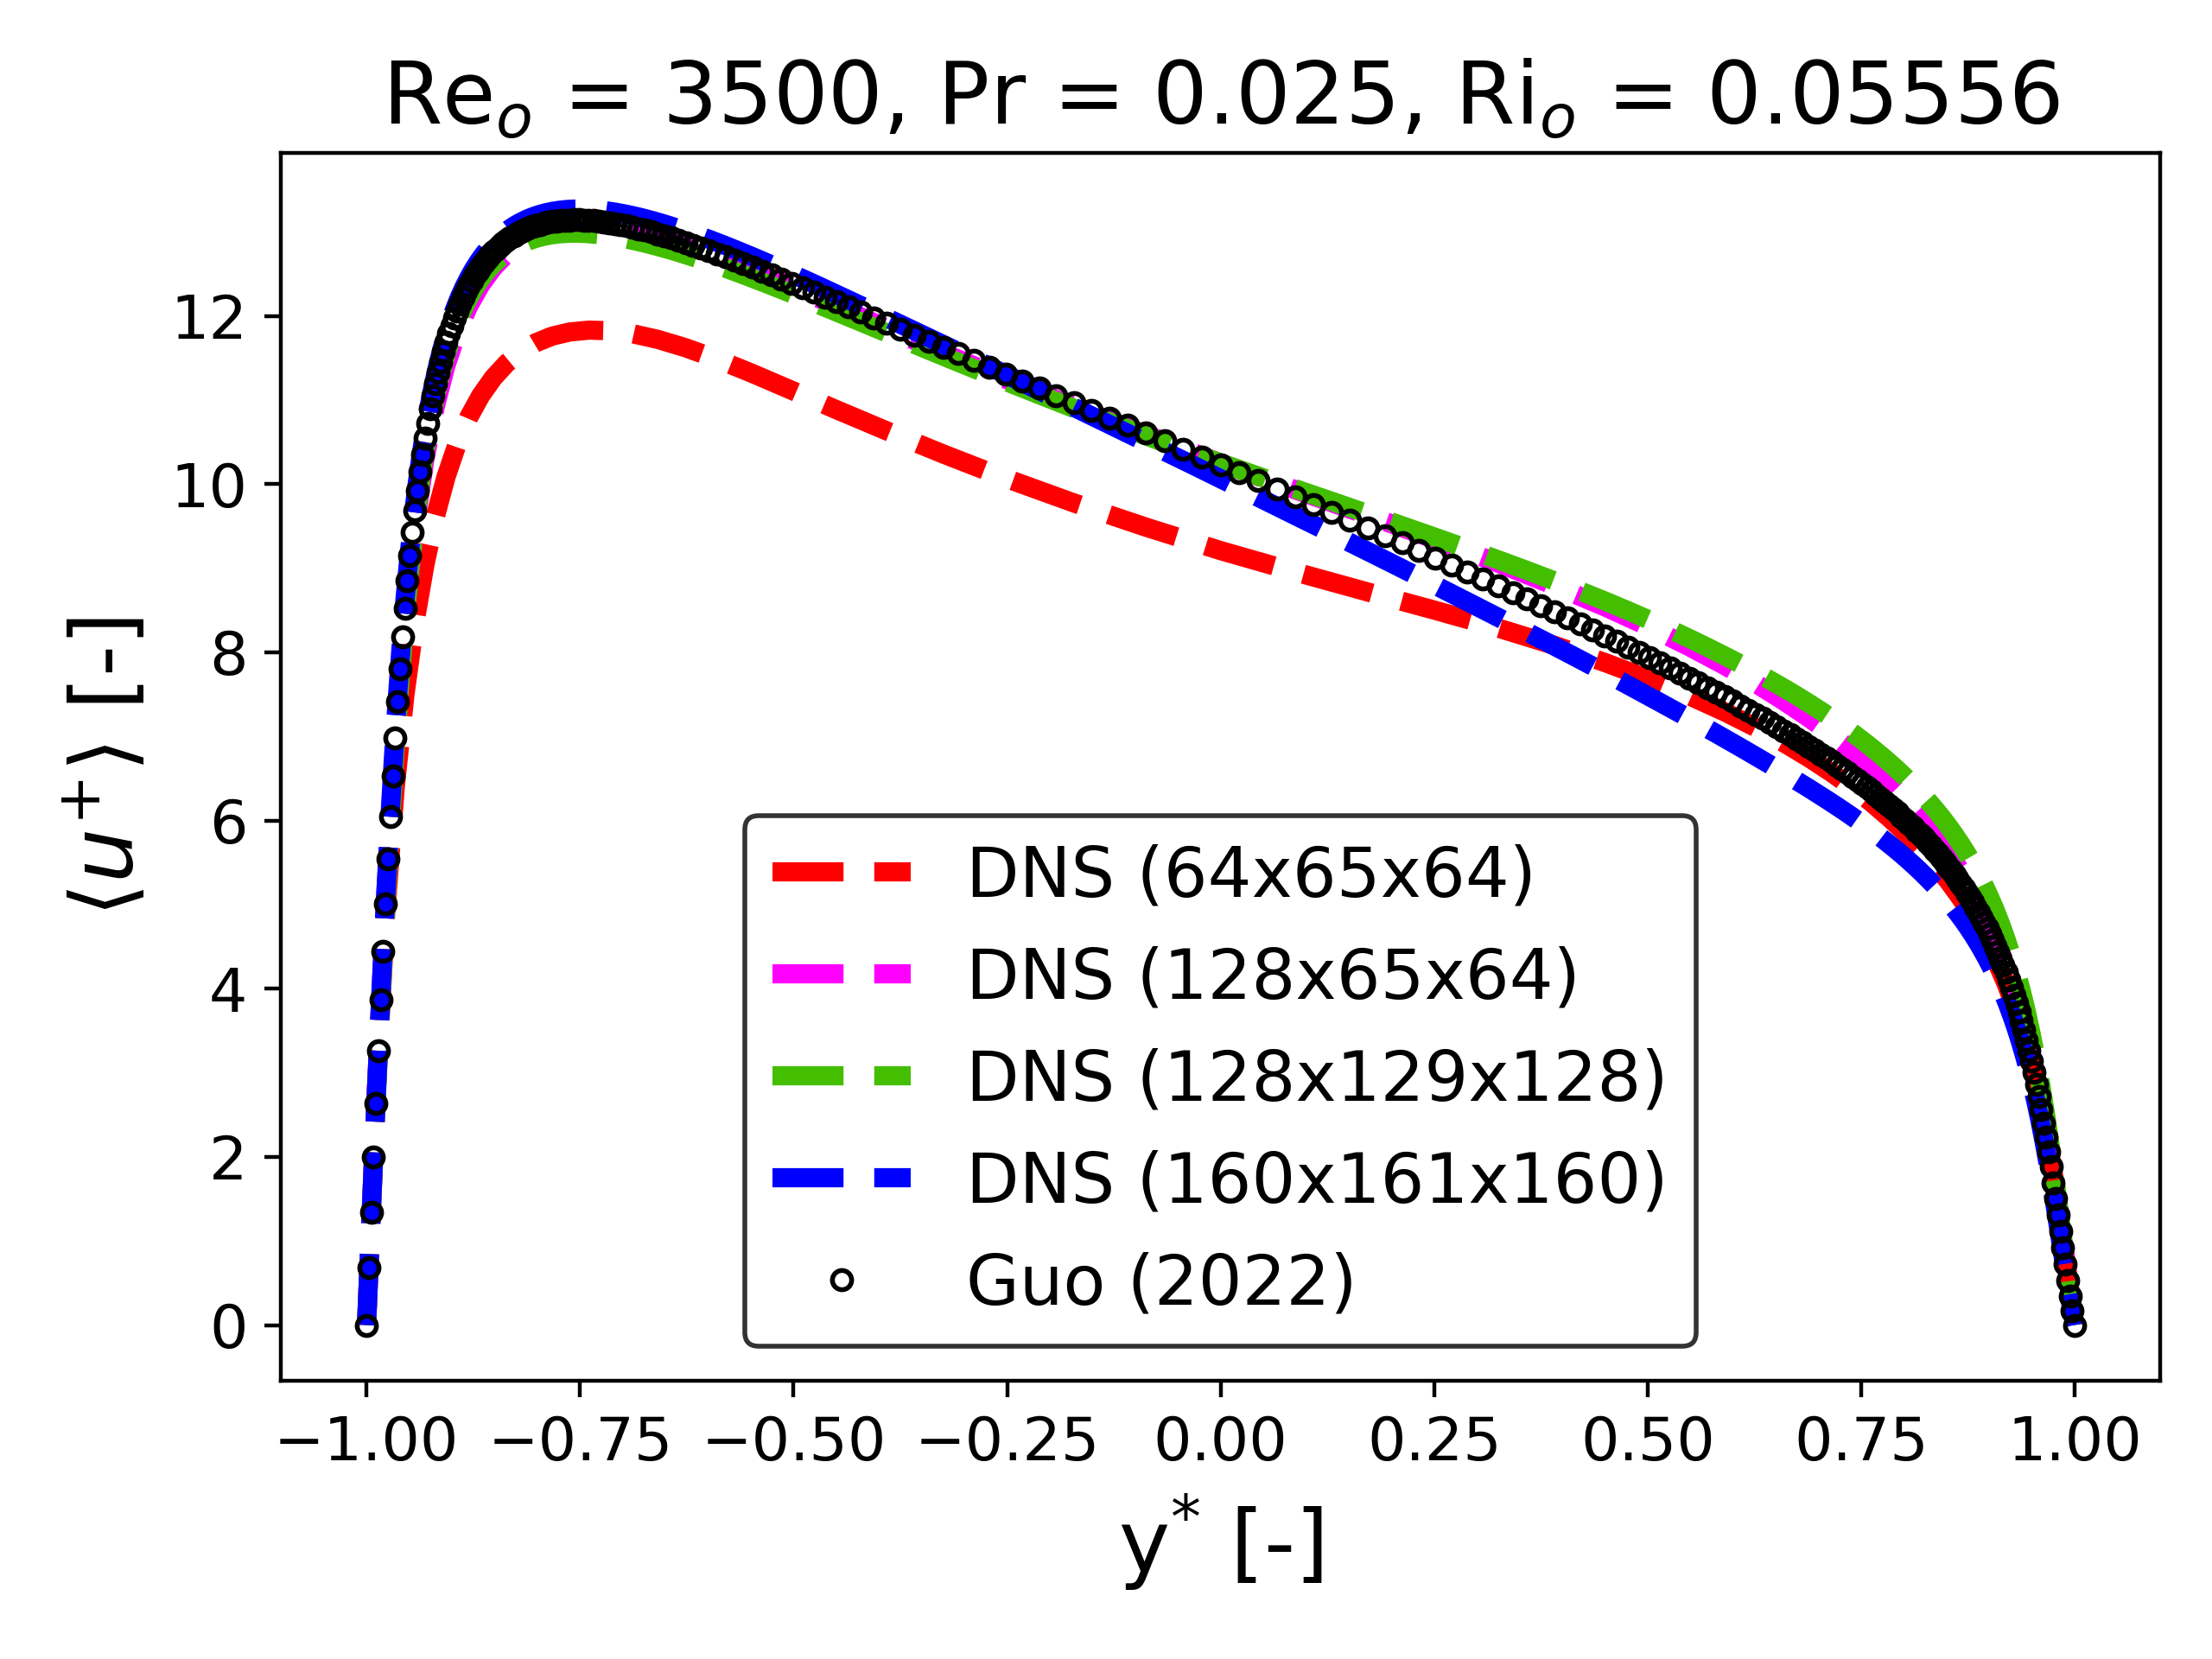
\includegraphics[width=0.49\textwidth]{results/guo/rib025/mct_upmean.png}
    \label{fig:phi_mean_guo}}  
  \subfloat[]{
    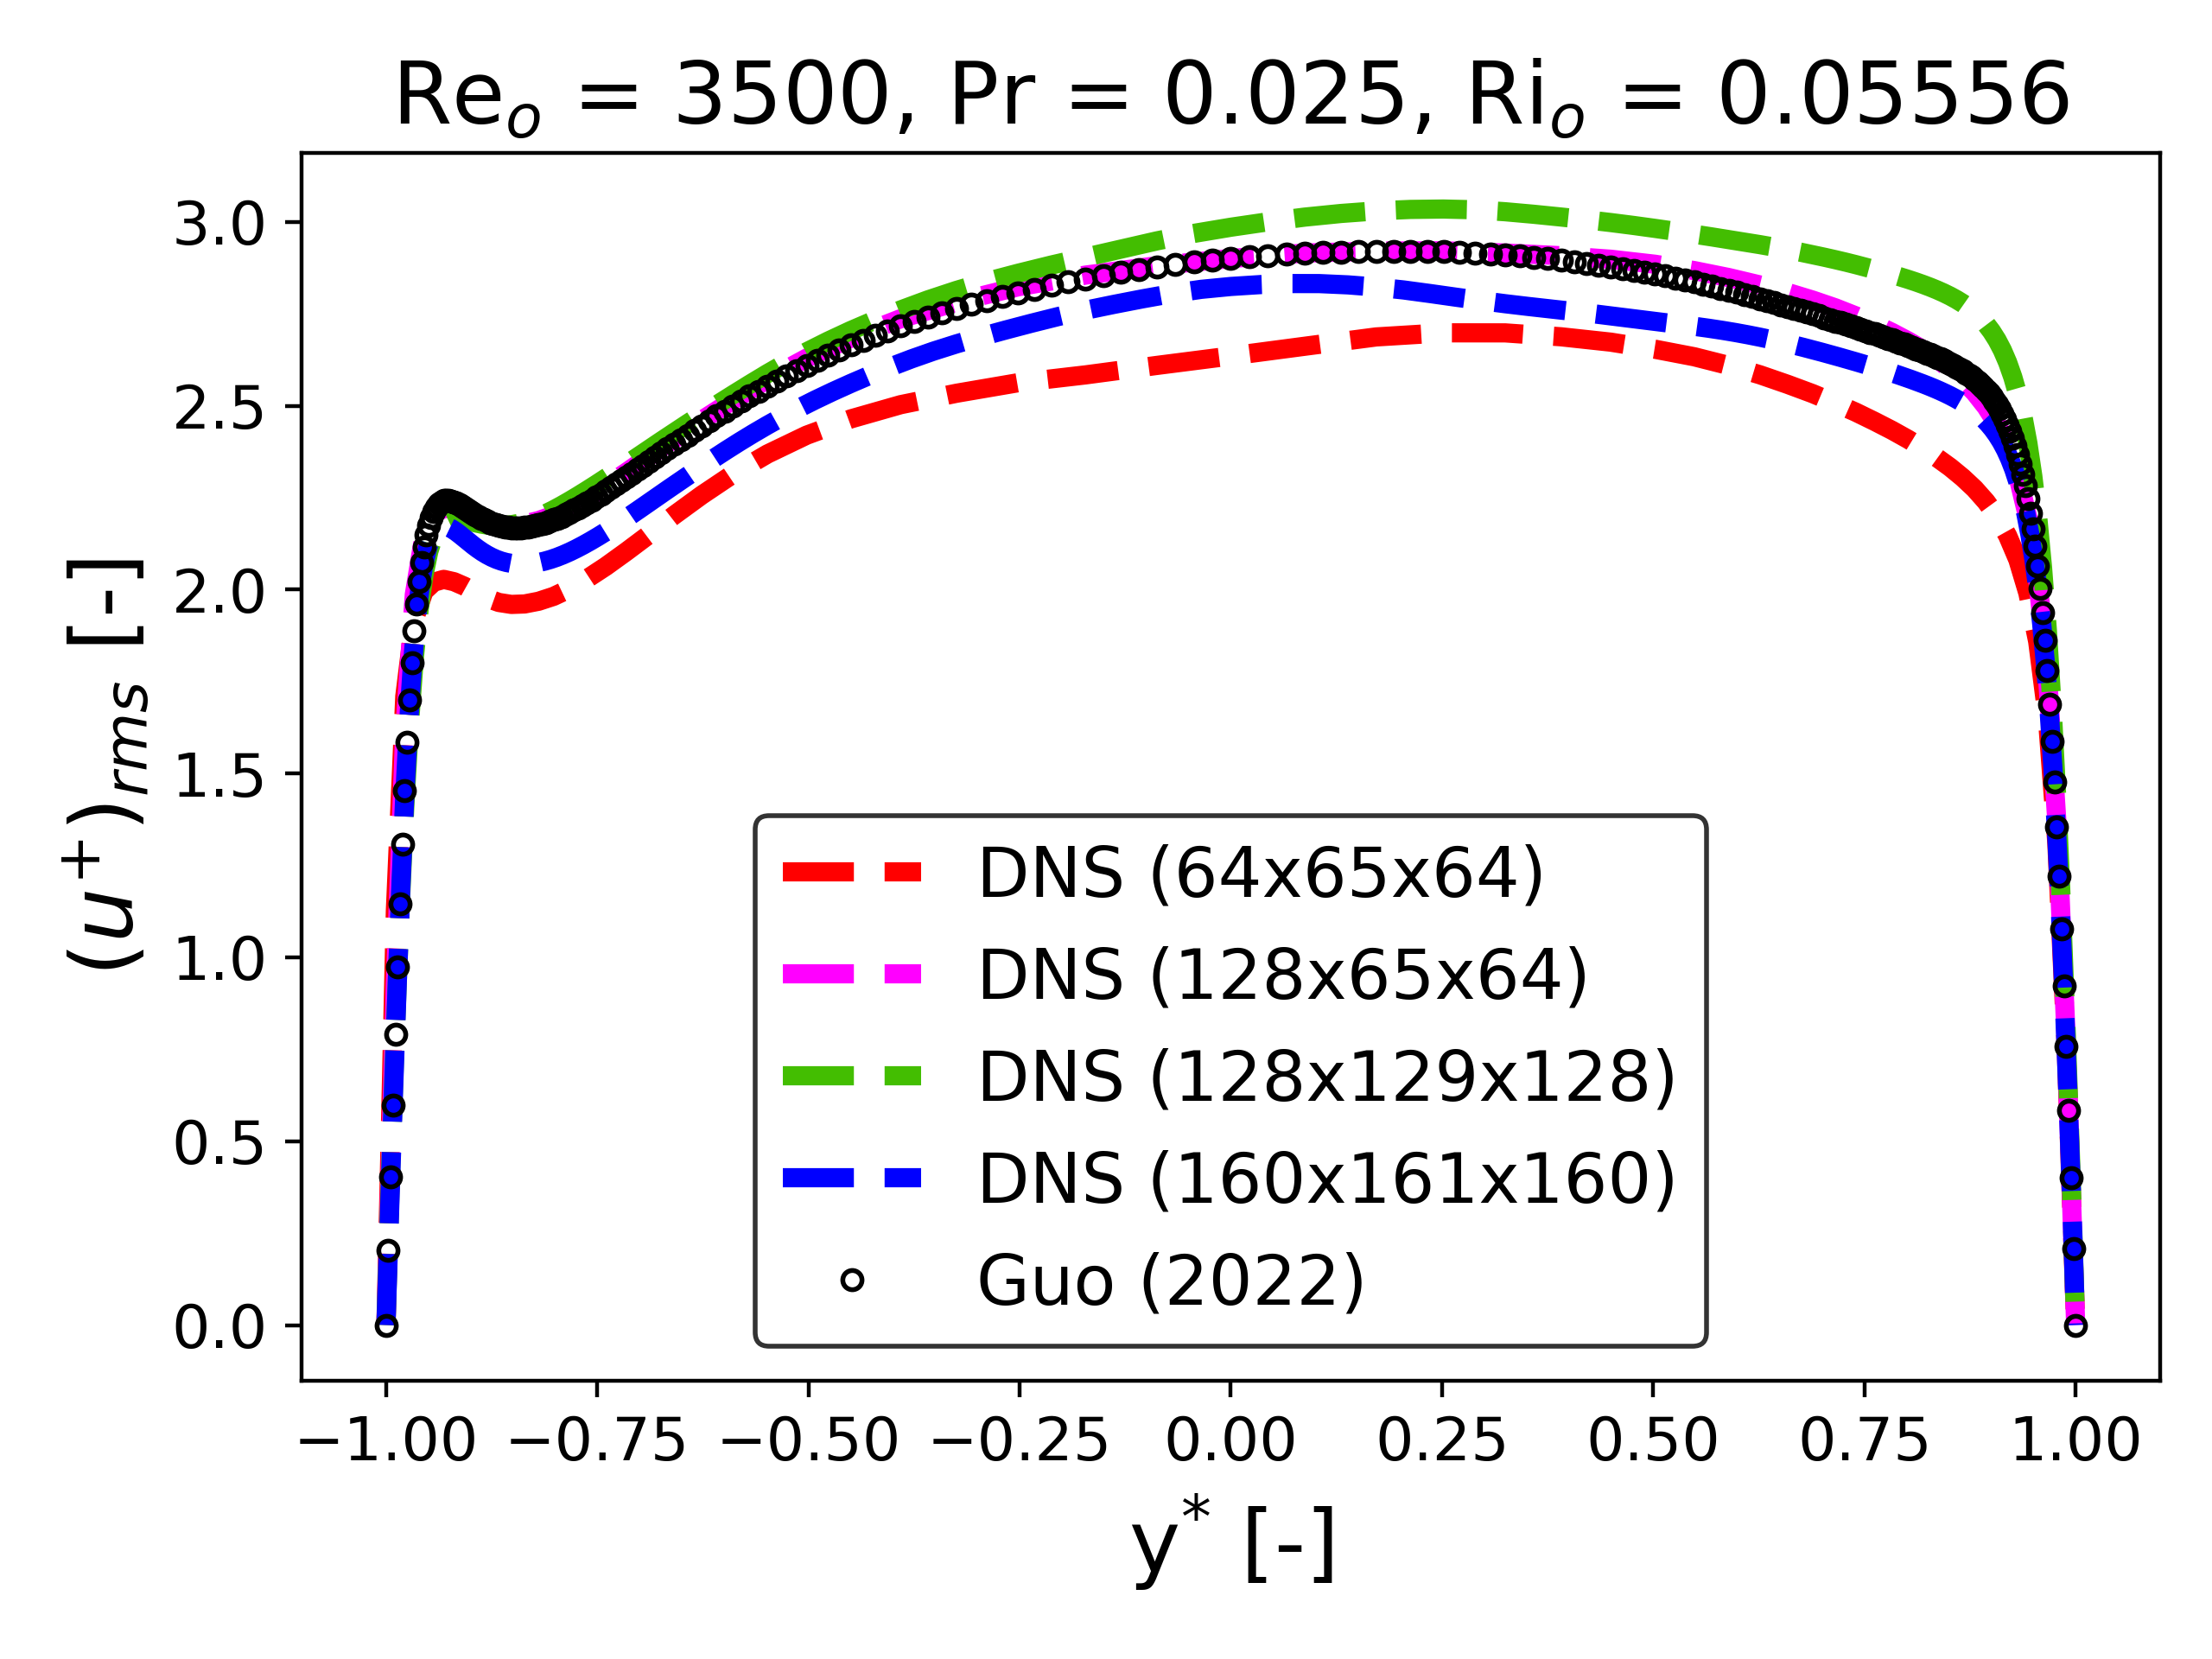
\includegraphics[width=0.49\textwidth]{results/guo/rib025/mct_uprms.png}
    \label{fig:phi_rms_guo}} 
 
  \subfloat[]{
    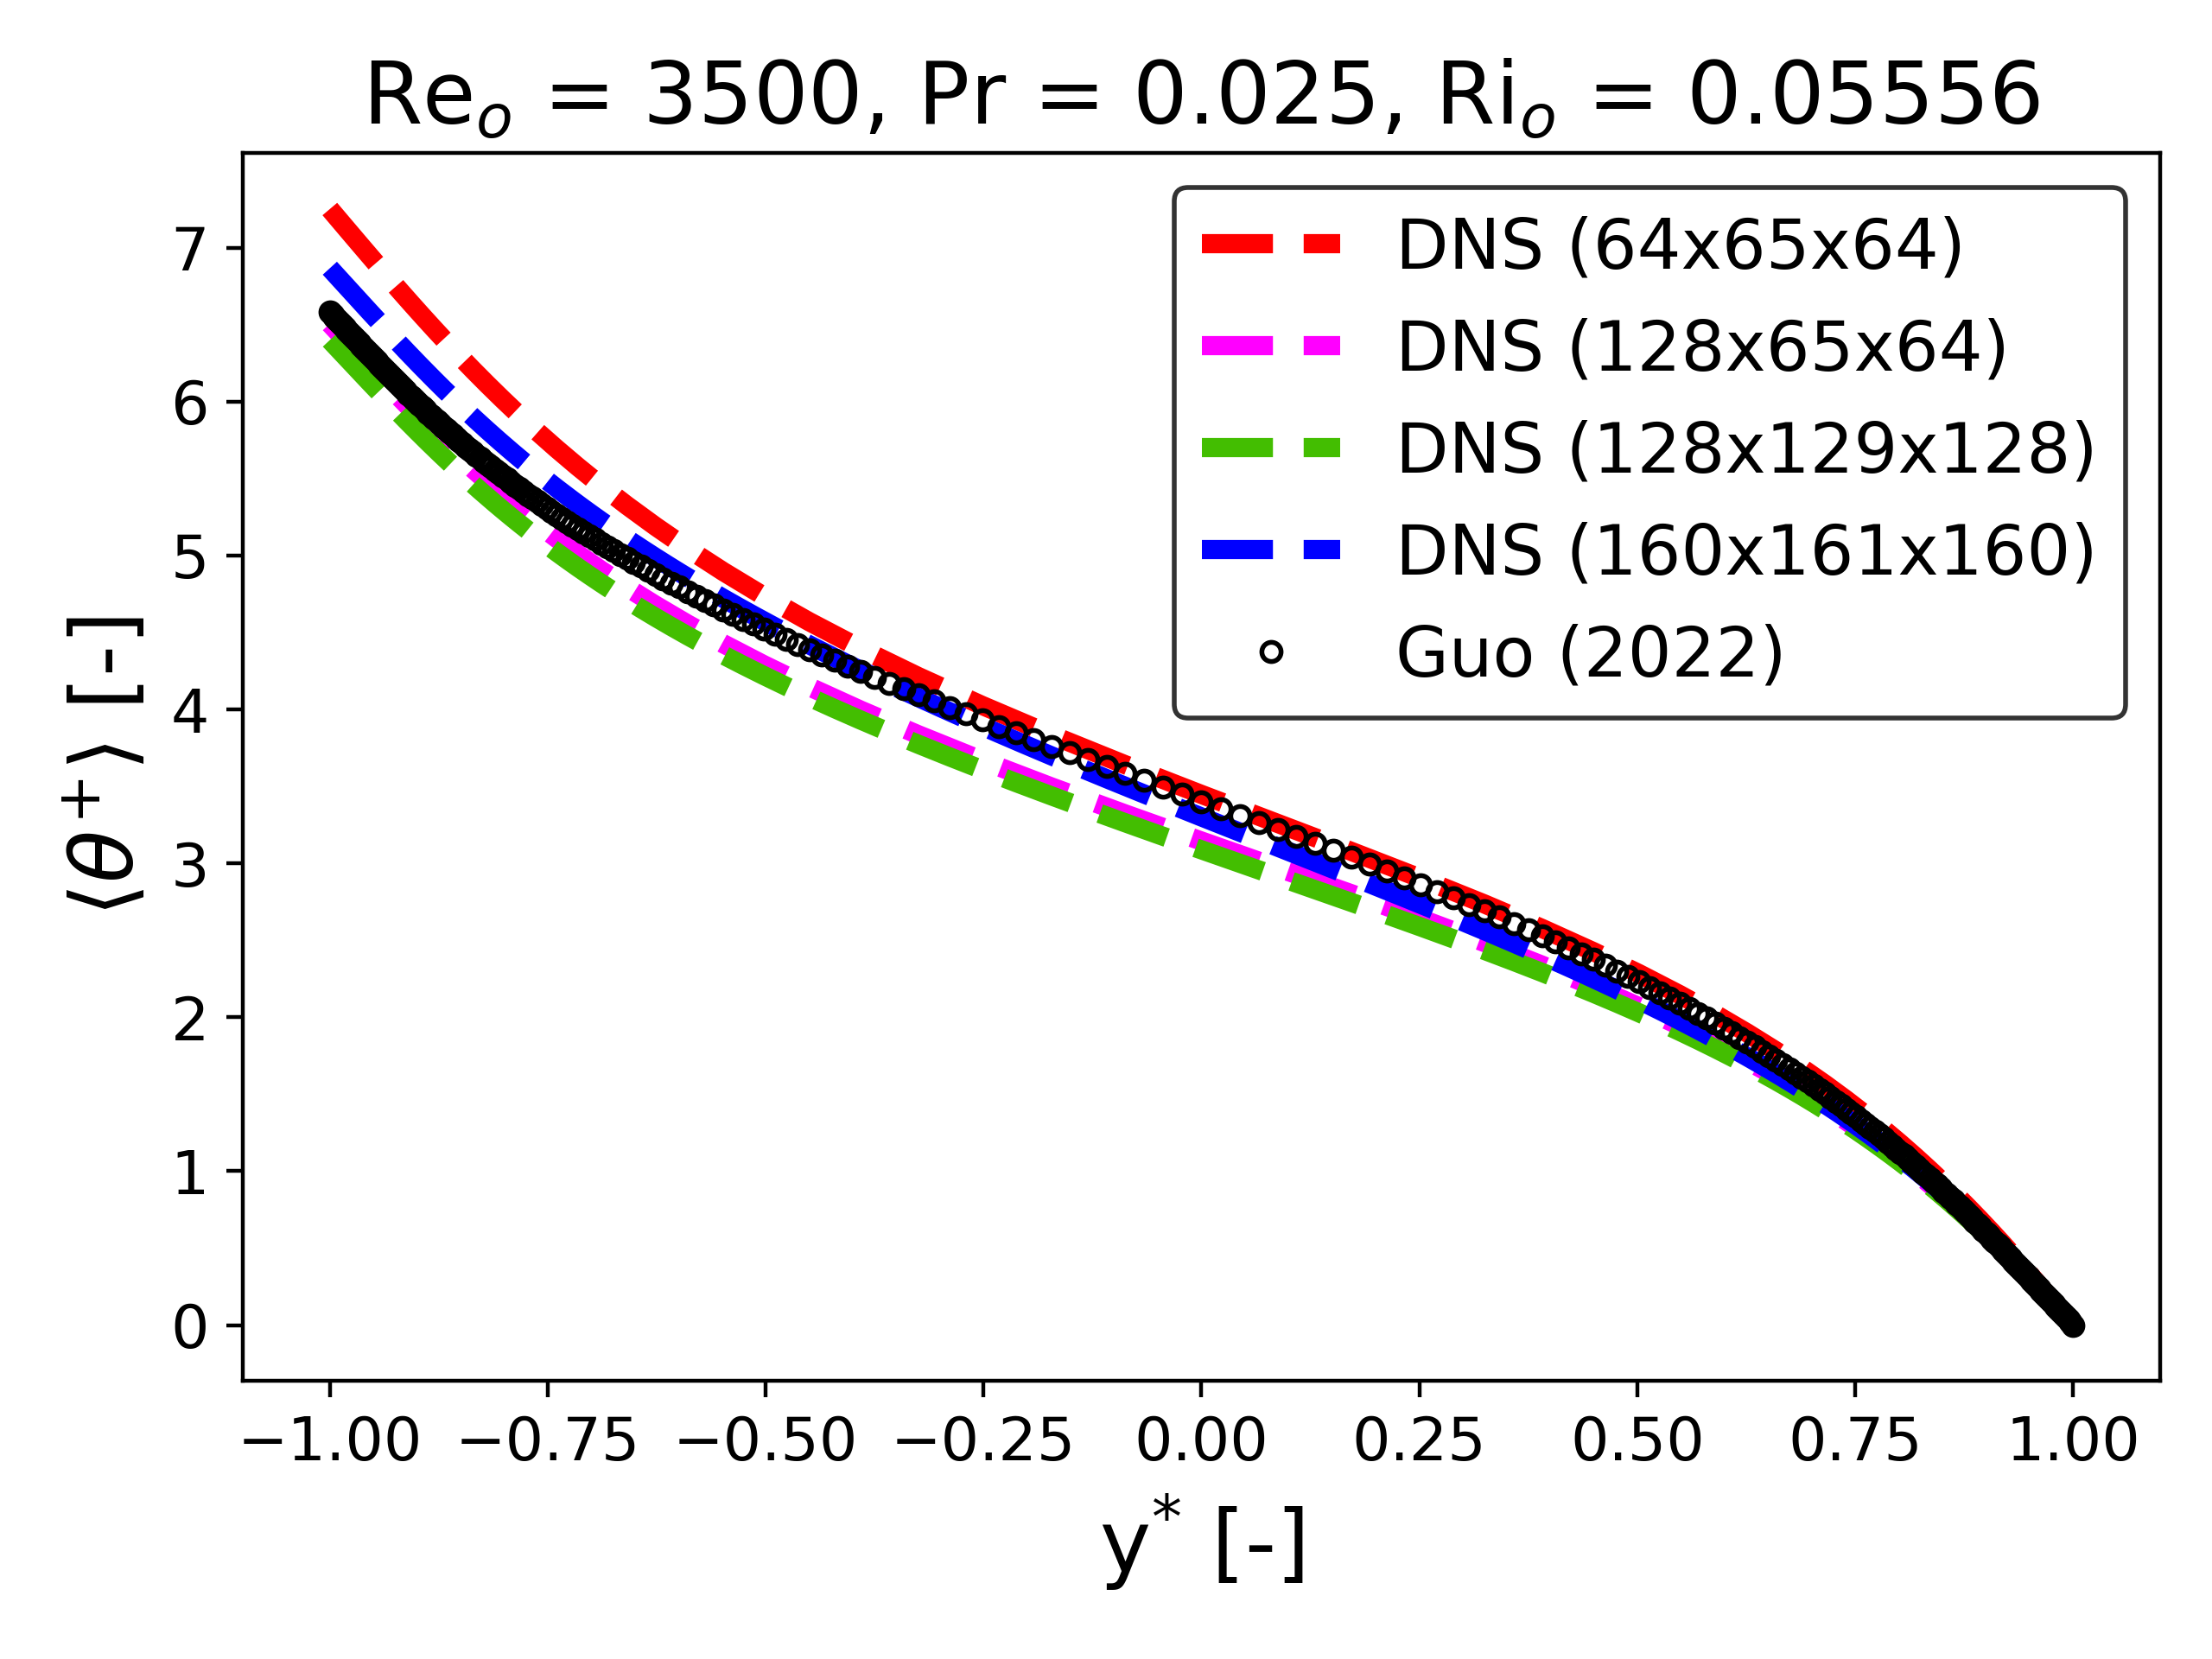
\includegraphics[width=0.49\textwidth]{results/guo/rib025/mct_theta.png}
    \label{fig:phi_mean_guo}}  
  \subfloat[]{
    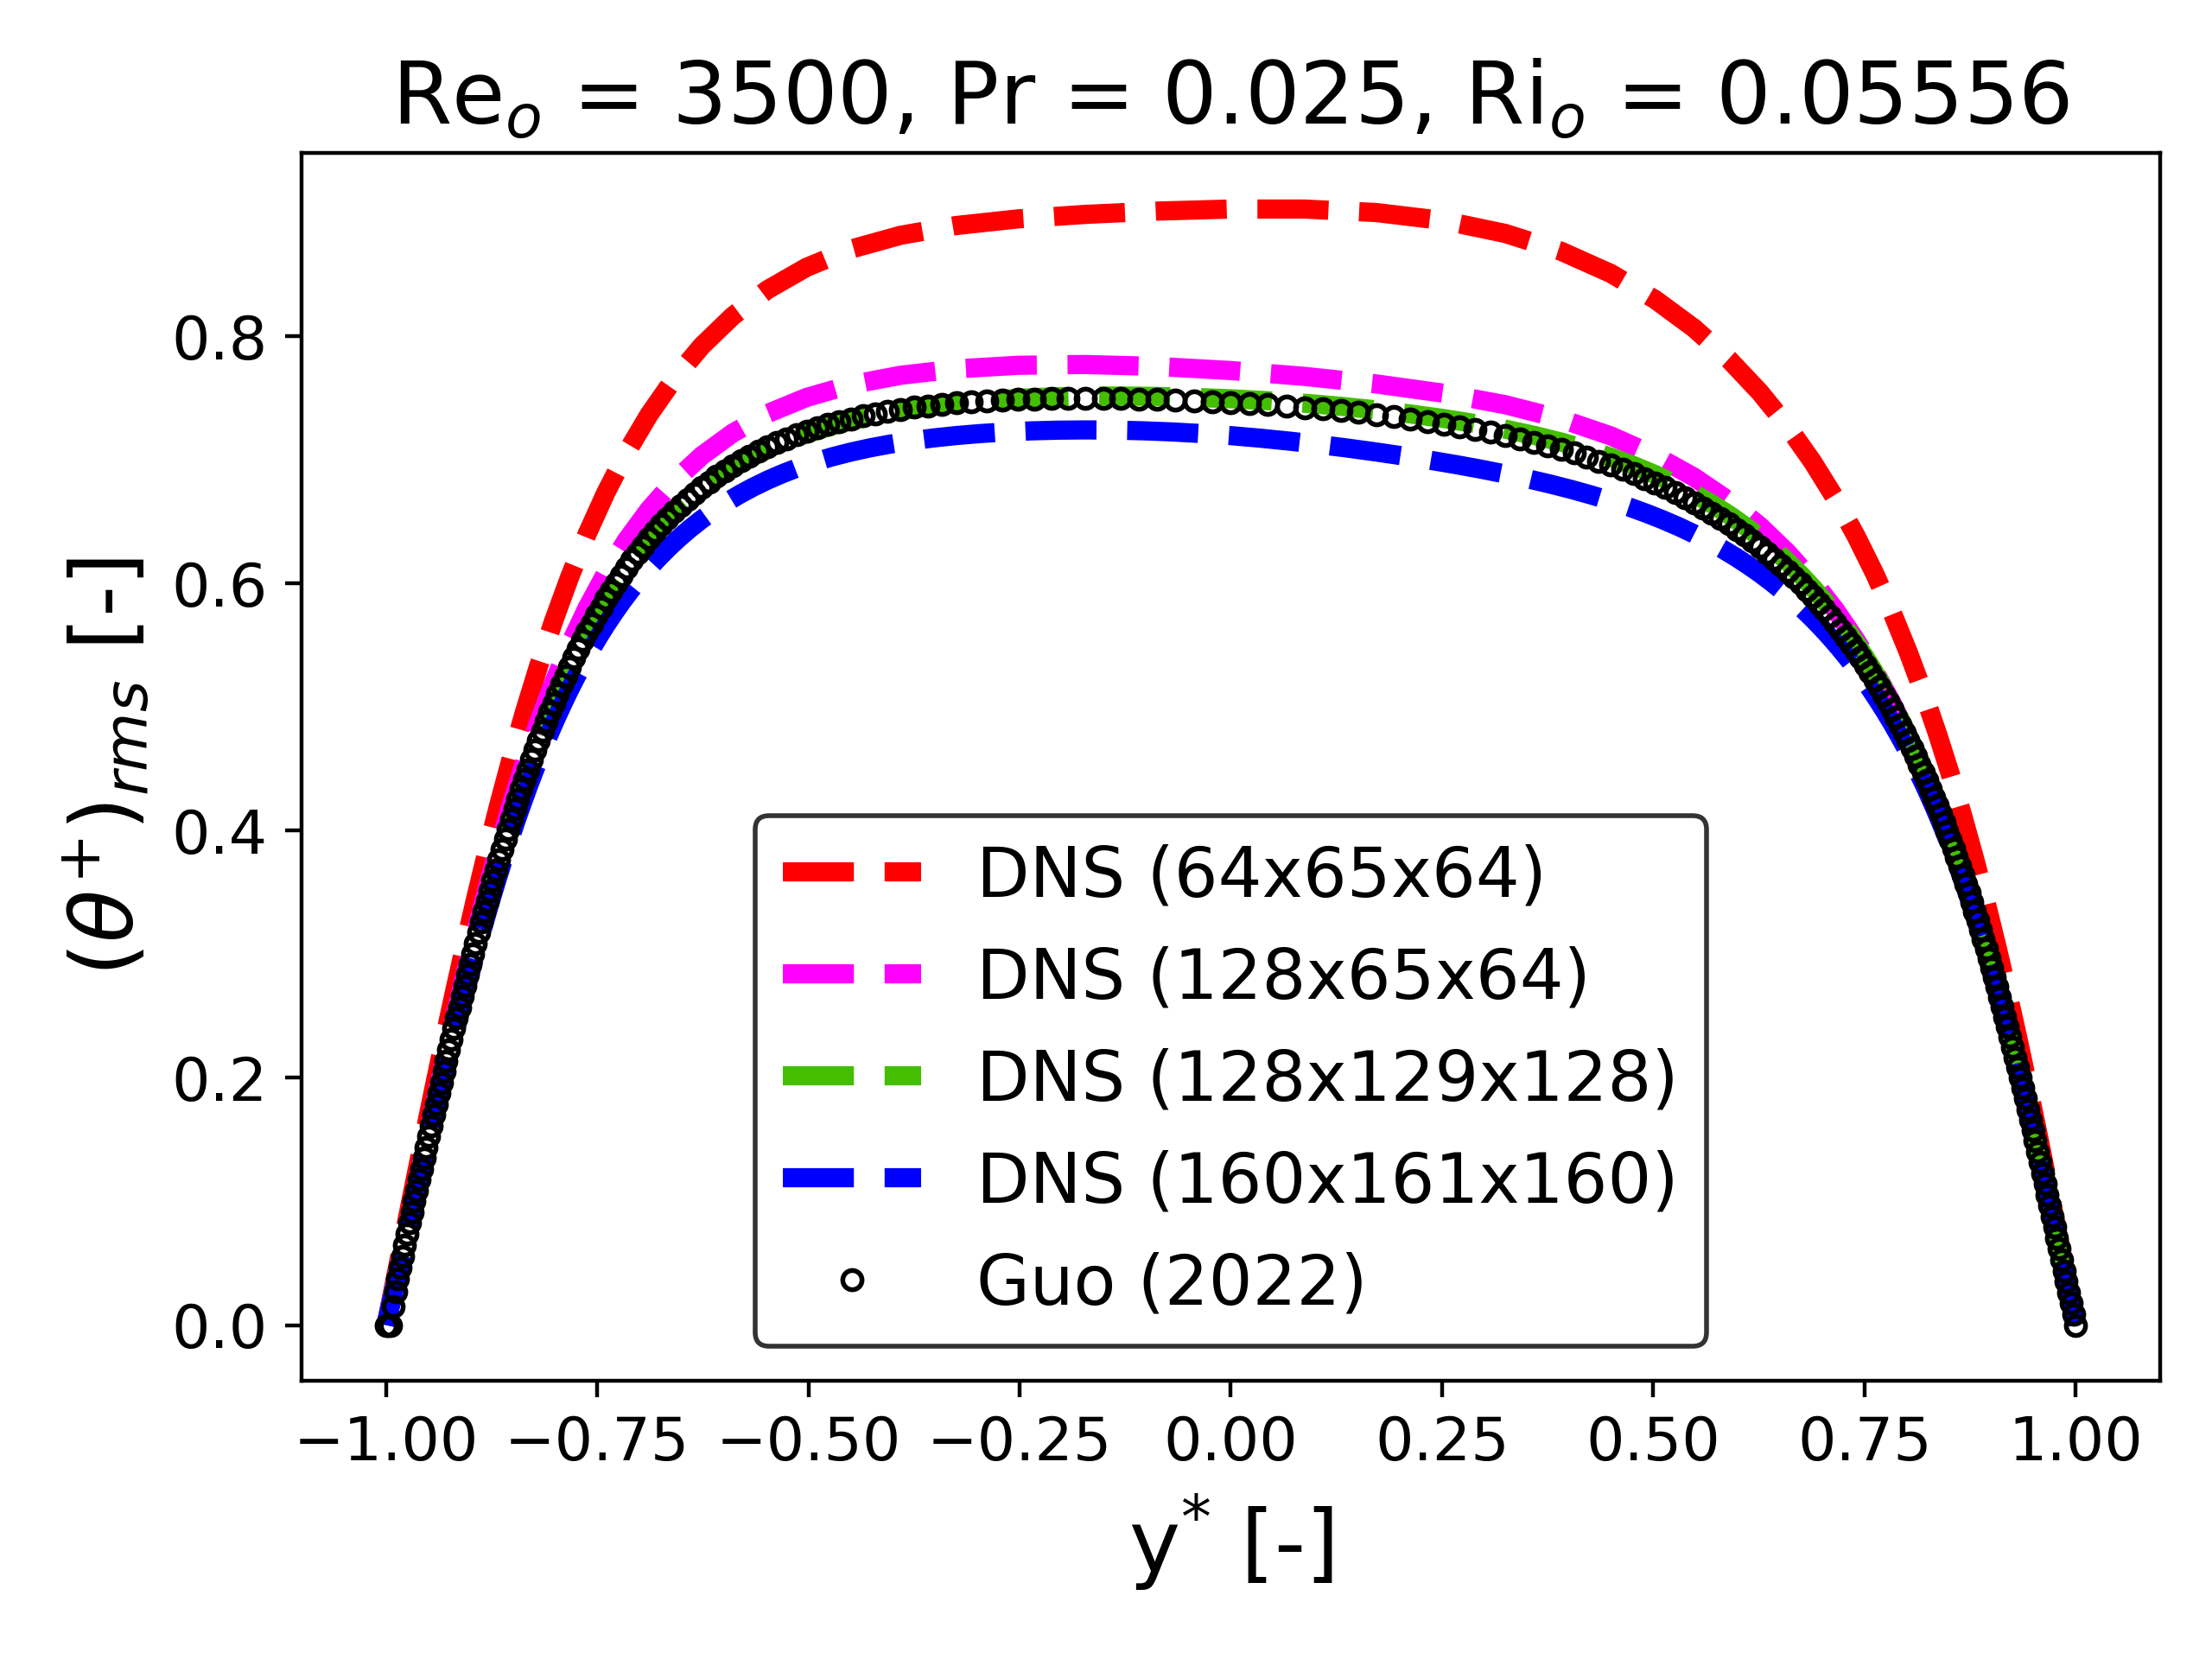
\includegraphics[width=0.49\textwidth]{results/guo/rib025/mct_thetap_rms.png}
    \label{fig:phi_rms_guo}}  

  \subfloat[]{
    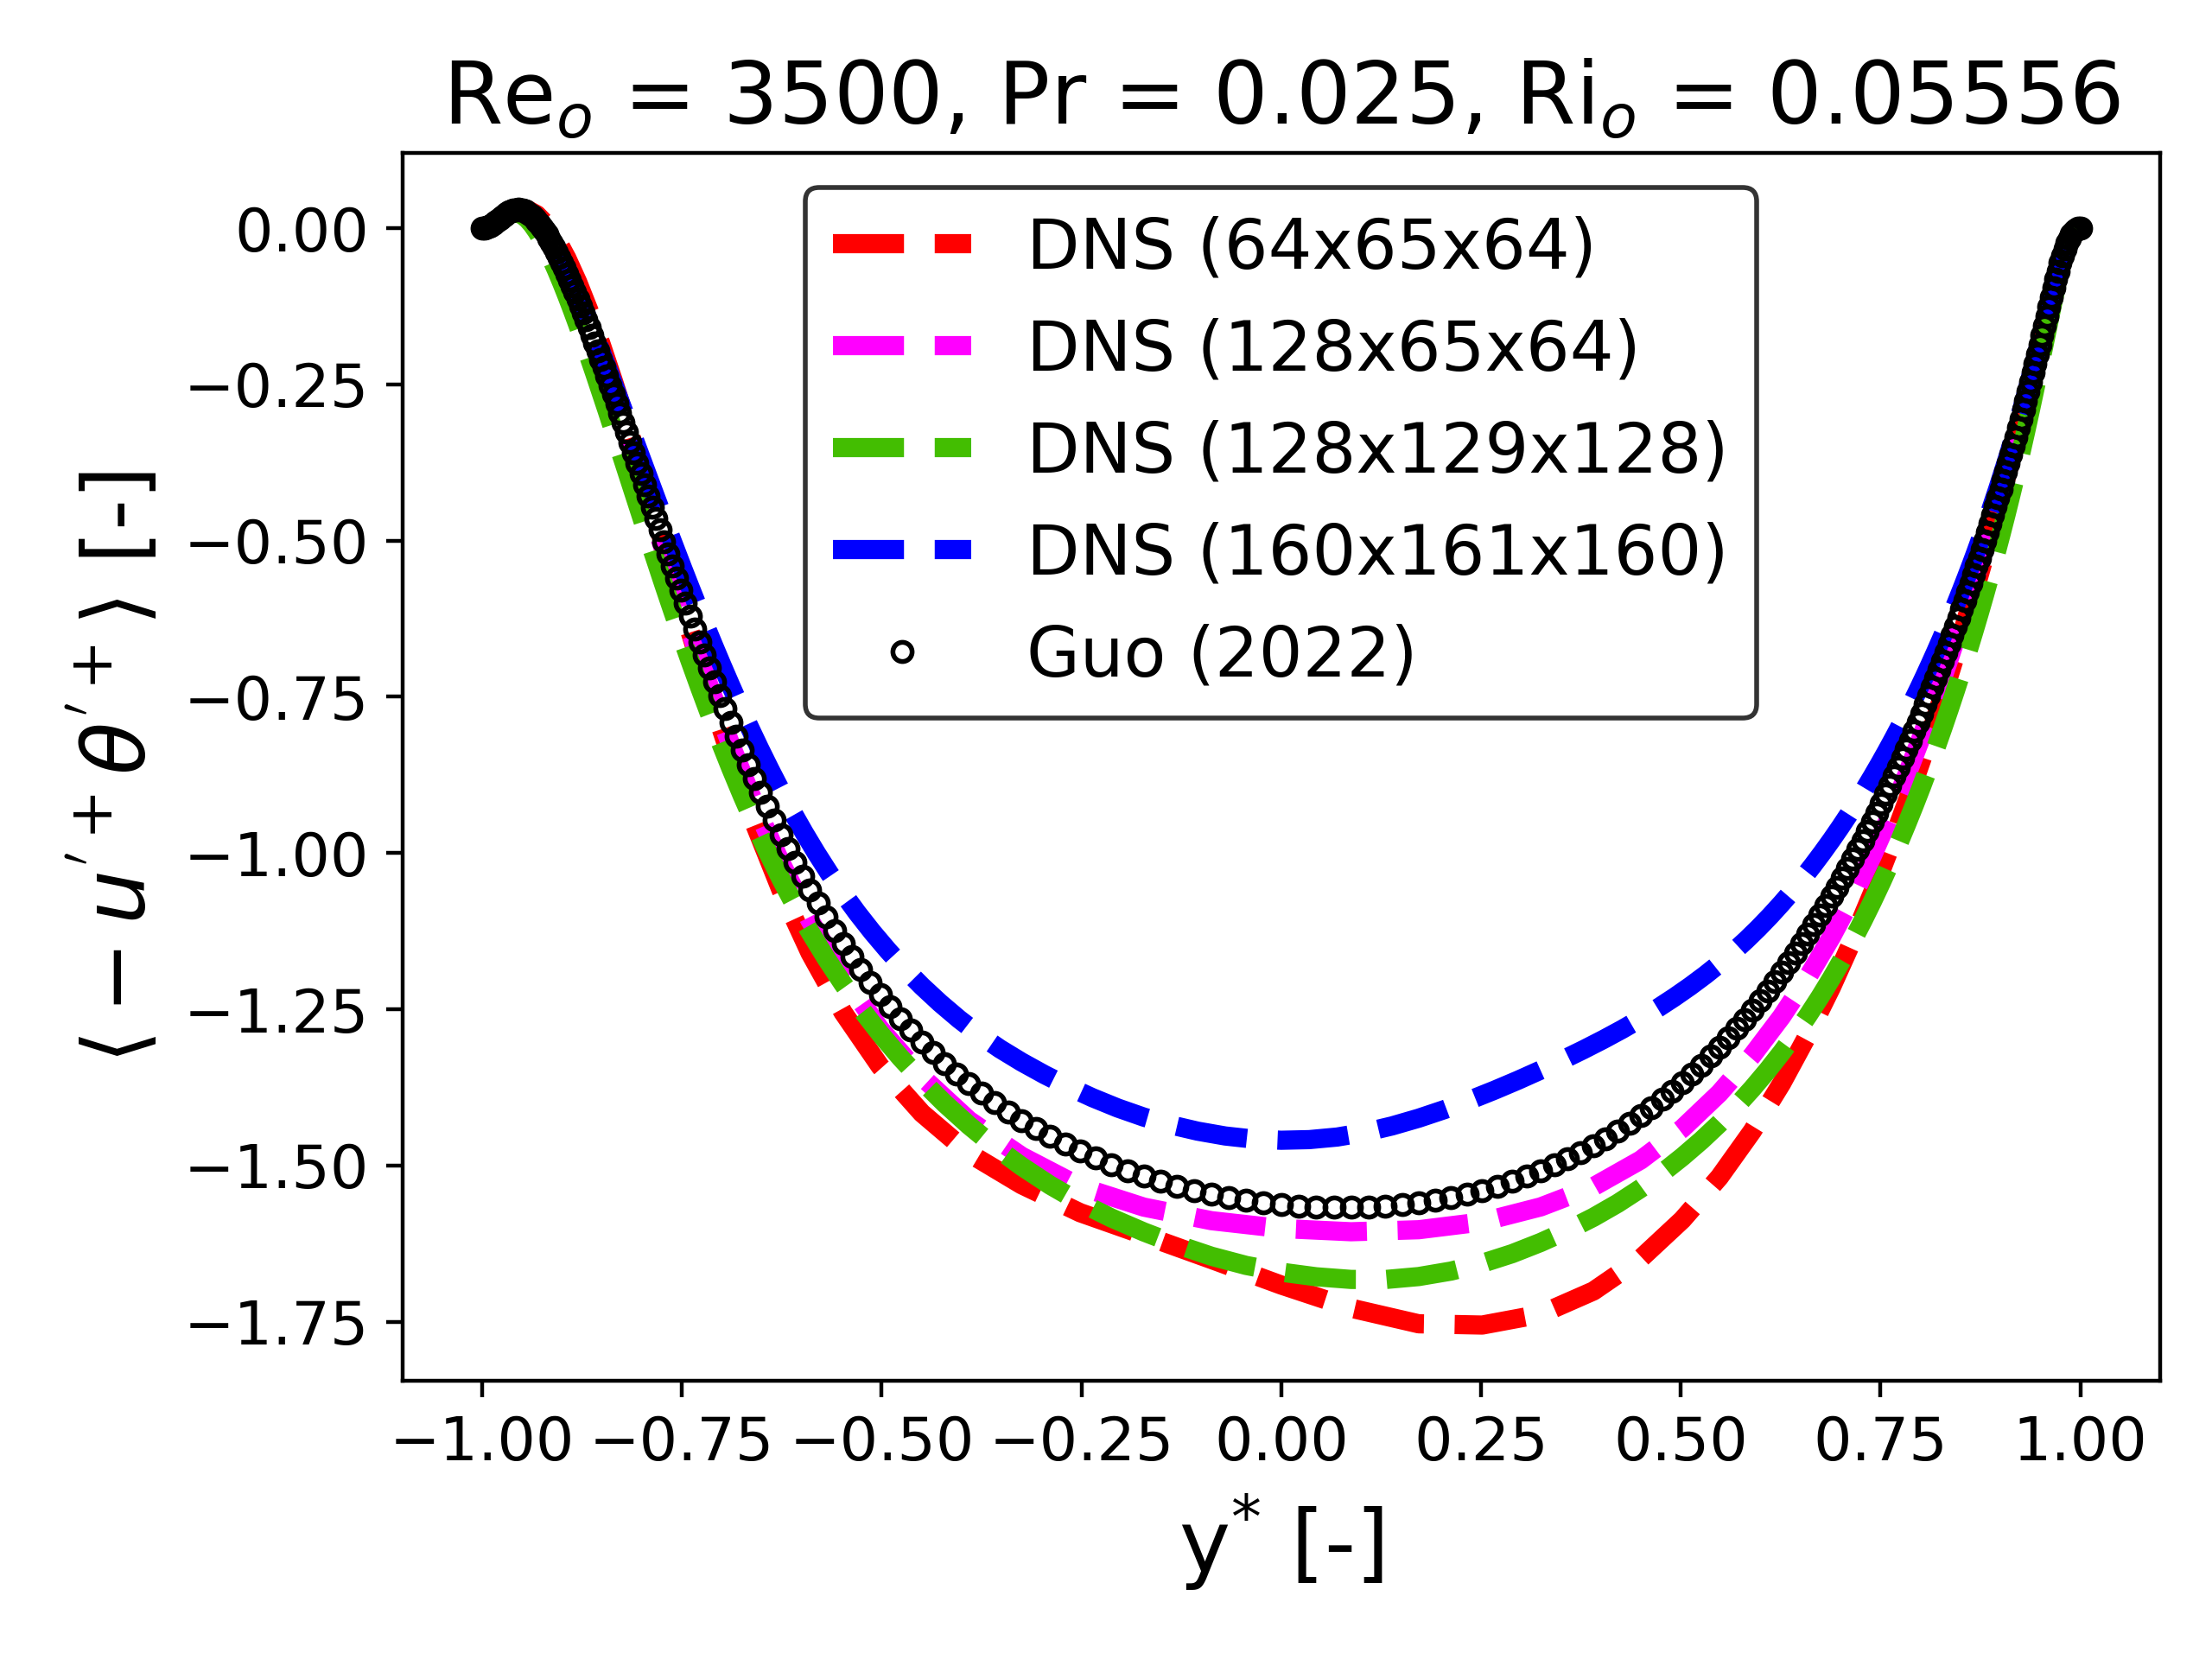
\includegraphics[width=0.49\textwidth]{results/guo/rib025/mct_up_thetap.png}
    \label{fig:phi_up_thetap_guo}}
  \subfloat[]{
    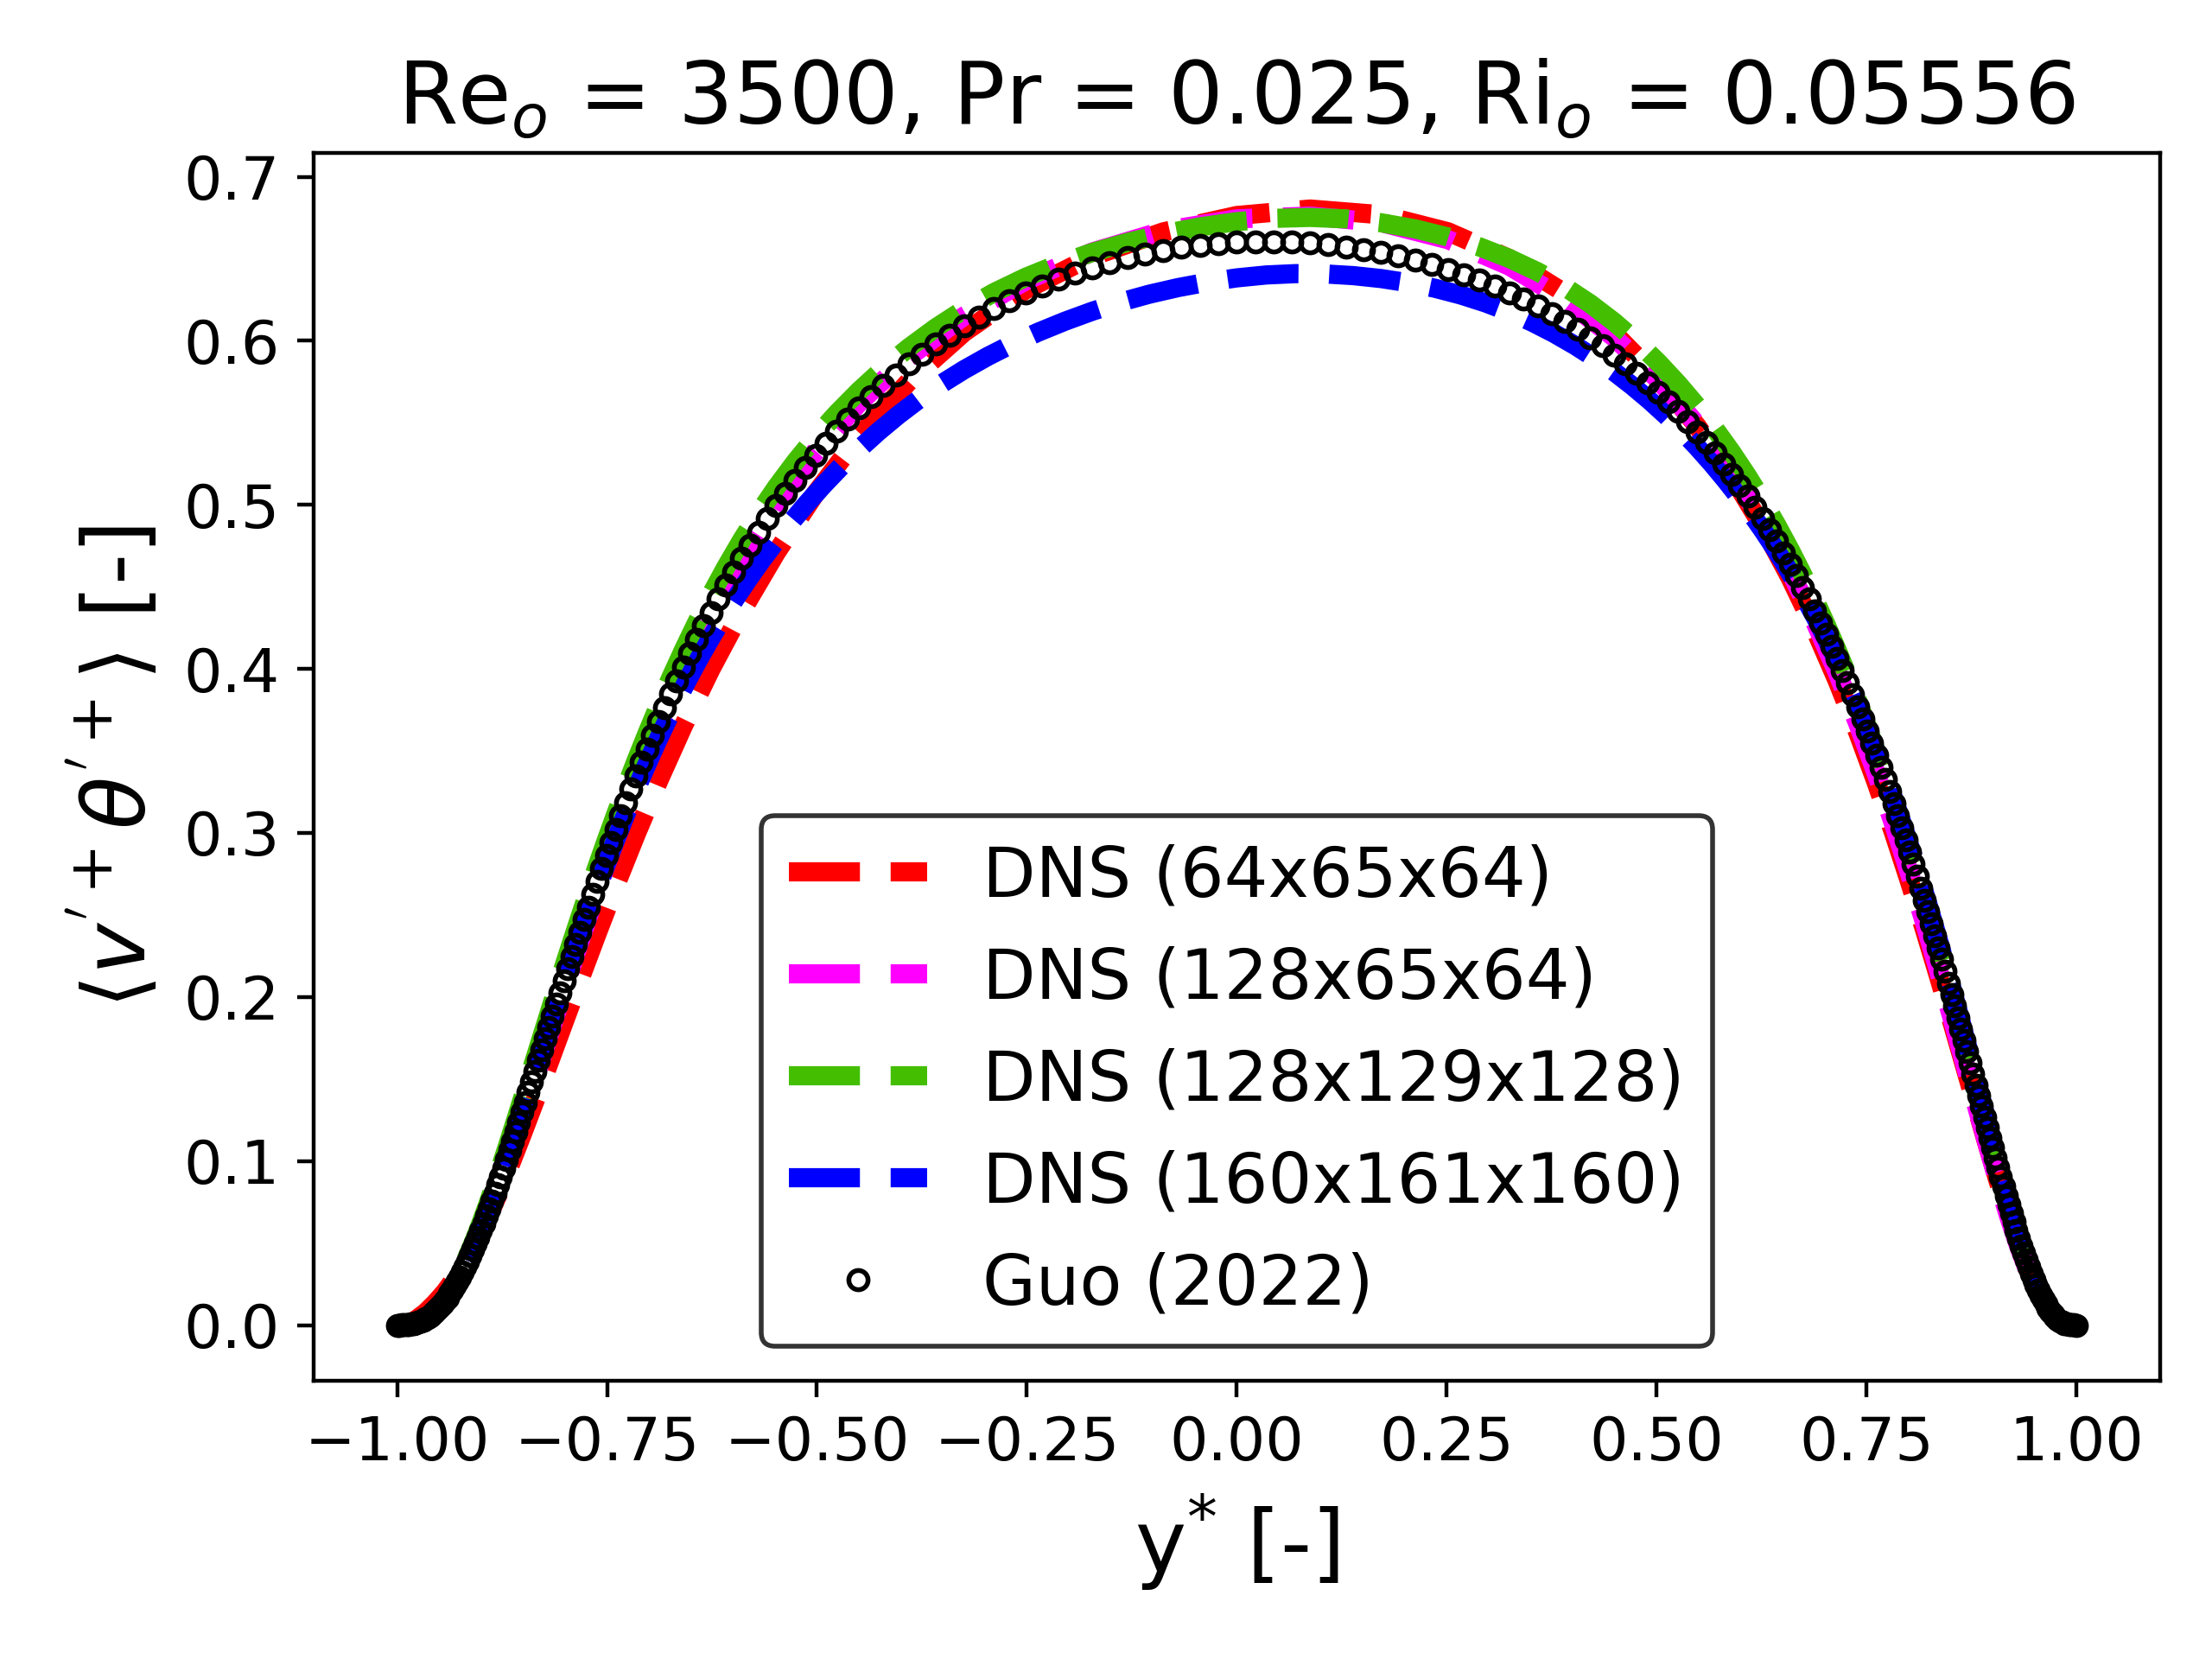
\includegraphics[width=0.49\textwidth]{results/guo/rib025/mct_vp_thetap.png}
    \label{fig:phi_vp_thetap_guo}}  
    
   \caption{a) Perfiles de temperatura media. b) Fluctuaciones de la temperatura. c) Perfiles de la velocidad media en la dirección de la corriente. d) Fluctuaciones de la velocidad en la dirección de la corriente. e) Flujo turbulento de calor en la dirección X. f) Flujo turbulento de calor en la dirección Y.} 
 
 \label{fig:guo}
\end{figure}
\end{comment}